% %% LyX 2.4.1 created this file.  For more info, see https://www.lyx.org/.
% %% Do not edit unless you really know what you are doing.
% \documentclass[onecolumn,english,american,compsoc]{IEEEtran}
% \usepackage[T1]{fontenc}
% \usepackage[utf8]{inputenc}
% \usepackage{geometry}
% \geometry{verbose,tmargin=1cm,bmargin=1cm,lmargin=1cm,rmargin=1cm}
% \usepackage{float}
% \usepackage{calc}
% \usepackage{amsmath}
% \usepackage{amsthm}
% \usepackage{amssymb}
% \usepackage{cancel}
% \usepackage{graphicx}

% \makeatletter

% %%%%%%%%%%%%%%%%%%%%%%%%%%%%%% LyX specific LaTeX commands.
% %% Because html converters don't know tabularnewline
% \providecommand{\tabularnewline}{\\}
% \floatstyle{ruled}
% \newfloat{algorithm}{tbp}{loa}
% \providecommand{\algorithmname}{Algorithm}
% \floatname{algorithm}{\protect\algorithmname}

% %%%%%%%%%%%%%%%%%%%%%%%%%%%%%% Textclass specific LaTeX commands.
% \newcommand{\lyxaddress}[1]{
% 	\par {\raggedright #1
% 	\vspace{1.4em}
% 	\noindent\par}
% }
% % \theoremstyle{plain}
% % \newtheorem{thm}{\protect\theoremname}
% % \theoremstyle{plain}
% % \newtheorem{prop}[thm]{\protect\propositionname}
% % \theoremstyle{plain}
% % \newtheorem{lem}[thm]{\protect\lemmaname}
% % \theoremstyle{plain}
% % \newtheorem{cor}[thm]{\protect\corollaryname}
% % \theoremstyle{definition}
% % \newtheorem{example}[thm]{\protect\examplename}

% %%%%%%%%%%%%%%%%%%%%%%%%%%%%%% User specified LaTeX commands.
% \usepackage{amsmath,amssymb,bm}
% \usepackage{tikz}
% \usetikzlibrary{arrows.meta,positioning,calc,fit,backgrounds}
% \pagestyle{empty}

% \definecolor{inputgray}{RGB}{76,84,92}
% \definecolor{predblue}{RGB}{42,104,145}
% \definecolor{predgreen}{RGB}{42,124,91}
% \definecolor{controlred}{RGB}{181,74,58}
% \definecolor{controlorange}{RGB}{196,116,42}
% \definecolor{fitpurple}{RGB}{102,75,145}
% \usepackage{adjustbox}

% \makeatother

% \usepackage{babel}
% \addto\captionsamerican{\renewcommand{\corollaryname}{Corollary}}
% \addto\captionsamerican{\renewcommand{\examplename}{Example}}
% \addto\captionsamerican{\renewcommand{\lemmaname}{Lemma}}
% \addto\captionsamerican{\renewcommand{\propositionname}{Proposition}}
% \addto\captionsamerican{\renewcommand{\theoremname}{Theorem}}
% \addto\captionsenglish{\renewcommand{\algorithmname}{Algorithm}}
% \addto\captionsenglish{\renewcommand{\corollaryname}{Corollary}}
% \addto\captionsenglish{\renewcommand{\examplename}{Example}}
% \addto\captionsenglish{\renewcommand{\lemmaname}{Lemma}}
% \addto\captionsenglish{\renewcommand{\propositionname}{Proposition}}
% \addto\captionsenglish{\renewcommand{\theoremname}{Theorem}}
% \providecommand{\corollaryname}{Corollary}
% \providecommand{\examplename}{Example}
% \providecommand{\lemmaname}{Lemma}
% \providecommand{\propositionname}{Proposition}
% \providecommand{\theoremname}{Theorem}

% \begin{document}
% \title{Dissociation of prediction and control in visual neuron}
% \author{Binxu Wang}
% \maketitle

% \lyxaddress{Kempner Institute, Harvard University}

\subsection{Motivation}

Linear regression on top of DNN features have been a classic way of
predicting visual and sensory neurons. 

Regression on many SOTA models yields very similar held out prediction
accuracy. 

Recent works found that though many models do have similar held-out
prediction accuracy, their ability to ``control'' neurons differs
dramatically. 

Here control refers to the following experiment, one let the model
$f(\mathbf{x})$ synthesize new inputs $\mathbf{x}^{*}$ to drive
the predicted response to a certain level $r^{*}$, and then test
whether the real neuron respond to $\mathbf{x}^{*}$ in the predicted
way in terms of Pearson r, R2, slope, etc. 

The experiment has following surprising findings 
\begin{itemize}
\item Models with similar heldout predicitivity exhibit largely different
control capability and very different image generation. 
\item Models that failed to control can still nicely predict the success
of other models. 
\item Models that failed to control usually synthesize more high frequency
patterns. 
\end{itemize}
In this paper, we are motivated to shine light on these phenomena
with a minimal linear model. 

We are going to show, these phenomena are not necessarily deep network
phenomena but could be recapitulated in a linear setting. 

Further the divergence of held-out prediction and control are there
in a Ridge regression setting. 

\section{Main results}

\subsection{Set up: Linear noisy teacher student and feature accentuation}

On a natural data distribution $(0,\Sigma)$ . The teacher weights
are $\beta^{\star}$, with Gaussian i.i.d. noise level $\sigma$ 
\[
y=\mathbf{x}^{\top}\beta^{\star}+\sigma\epsilon
\]

A student model is bias-free linear model with weight $\hat{\beta}$,
(or effective weight in linear feature case.) 
\[
f(\mathbf{x})=\mathbf{x}^{\top}\hat{\beta}
\]

For classic generalization, one sample new samples from basically
the population data distribution, and evaluate on it, thus the distribution
is 
\[
\mathcal{N}(0,\Sigma)
\]

For accentuation and control, one create self generated path and then
evaluate the prediction on it. 
\[
\mathbf{x}_{0}+\alpha\hat{\beta}
\]

In the main paper, we assume a single seed image which is $\mathbf{x}_{0}=0$,
and $\alpha$ is sampled from a distribution to make the \emph{predicted
model variance} matched with a target variance. e.g. 
\[
\mathrm{Var}[\alpha]\hat{\beta}^{\top}\hat{\beta}=\beta^{\star\top}\Sigma\beta^{\star}
\]

In supplementary, we will discuss the generalization to multi seed
images and non-centered seed image case. 

For peer review, model is evaluated on the accentuation path created
by other models with weight $\beta^{\prime}$, with similar structure
\[
\mathbf{x}_{0}+\alpha\beta^{\prime}
\]


\subsection{Intuition about the geometry}

With these structure we can already construct various cases where
two students $\hat{\beta}_{1},\hat{\beta}_{2}$ result in the same
prediction and accuracy, but with diverse control scores. 

As long as the weight difference is along some low var dimension of
data $\Sigma$, then prediction will be not sensitive to it while
control will be very sensitive to it. 

\subsection{Structure of the generalization and accentuation error}

Using the Lemma \ref{lem:pred_error}\ref{lem:R2_pred_obs}\ref{lem:Pearson-r_pred_obs}\ref{lem:linear_slope},
we can write down various form of evaluation metrics, MSE, R2, slope,
Pearson r, given the mean and covariance of a evaluation distribution. 

The difference between classic generalization, accentuation and peer
review can be seen via the (mean and) covariance of their evaluation
distribution. 

Using these difference we can write down the following table. 

We note that Pearson correlation is a degenerate metric when evaluating
on a single linear path, noiseless evaluation setting, so we focus
on other metrics, MSE, R2, slope. 
\begin{center}
\begin{tabular}{|c|c|c|c|c|c|c|}
\hline 
 & $\mu_{p}$ & $\Sigma_{p}$ & MSE & R2 & Slope & Pearson r\tabularnewline
\hline 
\hline 
General & $\mu_{p}$ & $\Sigma_{p}$ & $(\hat{\beta}-\beta^{\star})^{\top}\big(\mu_{p}\mu_{p}^{\top}+\Sigma_{p}\big)(\hat{\beta}-\beta^{\star})$ & $1-\frac{(\hat{\beta}-\beta^{\star})^{\top}\big(\mu_{p}\mu_{p}^{\top}+\Sigma_{p}\big)(\hat{\beta}-\beta^{\star})}{\beta^{\star}{}^{\top}\Sigma_{p}\beta^{\star}}$ & $\frac{\hat{\beta}{}^{\top}\Sigma_{p}\beta^{\star}}{\hat{\beta}{}^{\top}\Sigma_{p}\hat{\beta}}$ & $\frac{\hat{\beta}{}^{\top}\Sigma_{p}\beta^{\star}}{\sqrt{(\hat{\beta}{}^{\top}\Sigma_{p}\hat{\beta})(\beta^{\star}{}^{\top}\Sigma_{p}\beta^{\star})}}$\tabularnewline
\hline 
Generalization & $0$ & $\Sigma$ & $(\hat{\beta}-\beta^{\star})^{\top}\Sigma(\hat{\beta}-\beta^{\star})$ & $1-\frac{(\hat{\beta}-\beta^{\star})^{\top}\Sigma(\hat{\beta}-\beta^{\star})}{\beta^{\star}{}^{\top}\Sigma\beta^{\star}}$ & $\frac{\hat{\beta}{}^{\top}\Sigma\beta^{\star}}{\hat{\beta}{}^{\top}\Sigma\hat{\beta}}$ & $\frac{\hat{\beta}{}^{\top}\Sigma\beta^{\star}}{\sqrt{(\hat{\beta}{}^{\top}\Sigma\hat{\beta})(\beta^{\star}{}^{\top}\Sigma\beta^{\star})}}$\tabularnewline
\hline 
Accentuation & $0$ & $\mathrm{Var}[\alpha]\hat{\beta}\hat{\beta}^{\top}$ & $\mathrm{Var}[\alpha]\big(\hat{\beta}^{\top}(\hat{\beta}-\beta^{\star})\big)^{2}$ & $1-\big(\frac{\hat{\beta}^{\top}\hat{\beta}}{\hat{\beta}^{\top}\beta^{\star}}-1\big)^{2}$ & $\frac{\hat{\beta}^{\top}\beta^{\star}}{\hat{\beta}^{\top}\hat{\beta}}$ & $1$ or $nan$\tabularnewline
\hline 
Peer review & $0$ & $\mathrm{Var}[\alpha]\beta^{\prime}\beta^{\prime}{}^{\top}$ & $\mathrm{Var}[\alpha^{\prime}]\big(\beta^{\prime}{}^{\top}(\hat{\beta}-\beta^{\star})\big)^{2}$ & $1-\big(\frac{{\beta^\prime}^{\top}\hat{\beta}}{{\beta^\prime}^{\top}\beta^{\star}}-1\big)^{2}$ & $\frac{\beta^{\prime}{}^{\top}\beta^{\star}}{\beta^{\prime}{}^{\top}\hat{\beta}}$ & $1$ or $nan$\tabularnewline
\hline 
\end{tabular}
\par\end{center}

\subsection{Estimation of ratio of random variables}

One key structural observations is, 
\begin{prop}
All three metrics (MSE,R2,Slope) of accentuation and control error
are controlled by a scalar summary statistics, a ratio between two
inner product scalars 
\[
\frac{N}{D}=\frac{\hat{\beta}^{\top}\beta^{\star}}{\hat{\beta}^{\top}\hat{\beta}}
\]
\end{prop}
Thus so for accentuation, the central goal is to estimation of this
ratio. 

Note that $\hat{\beta}$ itself is a random variable, depending on
the noise realization $\eta$ and the data realization $X$. So this
ratio is a ratio of two random variables, and other metrics are also
nonlinear functions of this ratio. We will estimate this ratio via
2-3 ways 
\begin{enumerate}
\item \textbf{0th order ratio of DE:} In most\textbf{ }part of the paper,
as analytical tractability is needed, we will approximate expectation
of ratio via ratio of expectation 
\[
\mathbb{E}\Big[\frac{N}{D}\Big]\approx\frac{\mu_{N}}{\mu_{D}}
\]
This can be justified via concentration, when both N,D concentrates,
and Var and Cov are small w.r.t. the mean it's a viable choice. 
\item \textbf{DE of 2nd order correction}: Rarely we will incorporate 2nd
order correction to this estimate 
\[
\mathbb{E}\big[\frac{N}{D}\big]\approx\frac{\mu_{N}}{\mu_{D}}\Big(1-\frac{\mathrm{Cov}(D,N)}{\mu_{N}\mu_{D}}+\frac{\mathrm{Var}(D)}{\mu_{D}^{2}}\Big)
\]
\item \textbf{DE-Gaussian approximation}: Use DE to determine mean and cov
of $\hat{\beta}$, then approximate the distribution of $\hat{\beta}\dot{\sim}\mathcal{N}(m_{\beta,DE},V_{\beta,DE})$
then evaluate all the ratio and nonlinear functions via this monte
carlo averaging. 
\[
\mathbb{E}\Big[\frac{N}{D}\Big]\approx\mathbb{E}_{\hat{\beta}\dot{\sim}\mathcal{N}(m_{\beta,DE},V_{\beta,DE})}\Big[\frac{\hat{\beta}^{\top}\beta^{\star}}{\hat{\beta}^{\top}\hat{\beta}}\Big]
\]

\begin{enumerate}
\item Take n to 0 raise to power $(n-1)$
\end{enumerate}
\end{enumerate}

\subsection{Ridge regression}

Next we consider how the learning algorithm / estimator and noise
shapes this dissociation. 

We first consider ridge in the input space -- since intuitively ridge
regularization will penalize the non-aligned weights which alleviate
this problem. 
\begin{lem}
The ridge estimated solution reads 
\[
\hat{\beta}=\underbrace{(\hat{\Sigma}+\lambda I_{d})^{-1}\hat{\Sigma}\beta^{*}}_{\text{Signal}}+\underbrace{\sigma(\hat{\Sigma}+\lambda I_{d})^{-1}(\frac{1}{n}X^{\top}\eta)}_{\text{noise}}
\]
\end{lem}
\begin{prop}
Classic generalization (mean squared) error, has the following DE
\begin{align*}
E_{gen} & =(\hat{\beta}-\beta^{\star})^{\top}\Sigma(\hat{\beta}-\beta^{\star})\\
 & \asymp\frac{n}{n-\mathrm{df}_{2}\bigl(\kappa\bigr)}\kappa^{2}\beta^{*}{}^{\top}\bigl(\Sigma+\kappa I_{d}\bigr)^{-2}\Sigma\beta^{*}+\sigma^{2}\frac{\mathrm{df}_{2}(\kappa)}{n-\mathrm{df}_{2}(\kappa)}\\
 & =\frac{n}{n-\mathrm{df}_{2}\bigl(\kappa\bigr)}\big(\kappa^{2}B_{1,2}(\kappa)+\sigma^{2}\big)-\sigma^{2}
\end{align*}
which we will define as $E_{gen,DE}$. 
\end{prop}
This is different from the accentuation error
\begin{prop}
Accentuation and control error is characterized by the following ratio
$\frac{N}{D}$, where numerator and denominator each admits a deterministic
equivalence. 
\begin{align*}
\mu_{N}=\mathbb{E}_{X,\eta}\Big[N\Big] & \asymp\beta^{*\top}(\Sigma+\kappa I_{d})^{-1}\Sigma\beta^{*}\\
 & =B_{1,1}(\kappa)\\
\mu_{D}=\mathbb{E}_{X,\eta}\Big[D\Big] & \asymp\beta^{*\top}(\Sigma+\kappa I_{d})^{-2}\Sigma^{2}\beta^{*}+\frac{\mathrm{Tr}\Big[\Sigma(\Sigma+\kappa I_{d})^{-2}\Big]}{n-\mathrm{df}_{2}(\kappa)}\Big(\sigma^{2}+\kappa^{2}\beta^{*\top}(\Sigma+\kappa I_{d})^{-2}\Sigma\beta^{*}\Big)\\
 & =B_{2,2}(\kappa)+\frac{\mathrm{df}_{1,2}(\kappa)}{n-\mathrm{df}_{2}(\kappa)}\Big(\kappa^{2}B_{1,2}(\kappa)+\sigma^{2}\Big)\\
 & =B_{2,2}(\kappa)+\frac{1}{n}\mathrm{df}_{1,2}(\kappa)(E_{gen,DE}+\sigma^{2})
\end{align*}
So on the leading order it can be approximated by the ratio of the
two DE.
\[
\frac{N}{D}\approx\frac{\mu_{N}}{\mu_{D}}
\]
\end{prop}
This can be central quantity represented in various forms 
\begin{cor}
equivalent forms of the accentuation error
\begin{align*}
z_{acc}\approx\frac{\mu_{D}}{\mu_{N}}-1 & =\frac{B_{2,2}(\kappa)+\frac{1}{n}\mathrm{df}_{1,2}(\kappa)(E_{gen,DE}+\sigma^{2})}{B_{1,1}(\kappa)}-1\\
 & =\frac{-\kappa B_{1,2}(\kappa)+\frac{1}{n}\mathrm{df}_{1,2}(\kappa)(E_{gen,DE}+\sigma^{2})}{B_{1,1}(\kappa)}\\
 & =\frac{\sigma^{2}\mathrm{df}_{1,2}(\kappa)-n\lambda B_{1,2}(\kappa)}{(n-\mathrm{df}_{2}(\kappa))B_{1,1}(\kappa)}
\end{align*}
\end{cor}
%
We can see non-optimal regularization strength with noisy setting
can easily lead to catastrophic failure in control. But what if the
ridge parameter is optimized -- in reality people often do cross
validated selection in RidgeCV? 
\begin{lem}
The ridge parameter selection based on DE of generalization loss needs
to satisfy the first order condition
\[
(n-\mathrm{df}_{2}\bigl(\kappa\bigr))\kappa B_{2,3}(\kappa)=\mathrm{df}_{2,3}(\kappa)\big(\kappa^{2}B_{1,2}(\kappa)+\sigma^{2}\big)
\]
which can also be written through the generalization error at DE level.
\[
\kappa\frac{B_{2,3}(\kappa)}{\mathrm{df}_{2,3}(\kappa)}=\frac{1}{n}(E_{gen,DE}+\sigma^{2})
\]
\end{lem}
Further even if we select the best ridge parameter, the accentuation
error can still be written as 
\begin{prop}
When we select regularization parameter by minimizing generalization
error (RidgeCV), at this stationary point, accentuation error has
additional structure. and can be written as 
\begin{align*}
z_{acc,CV}\approx\frac{\mu_{D}}{\mu_{N}}-1 & =\frac{\kappa\mathrm{df}_{1,2}(\kappa)}{B_{1,1}(\kappa)}\Big(\frac{B_{2,3}(\kappa)}{\mathrm{df}_{2,3}(\kappa)}-\frac{B_{1,2}(\kappa)}{\mathrm{df}_{1,2}(\kappa)}\Big)\\
\end{align*}
\end{prop}

\subsection{Ridge Regression on Linear Feature }

When we consider feature space $F$ i.e. teacher remain the same,
while student is a linear function on a feature space 
\[
f(\mathbf{x})=w^{\top}F\mathbf{x}
\]

the effective weights is 
\[
\hat{\beta}=F^{\top}w
\]

With a feature space, the original teacher signal may not be representable.
So first we need to define a sense of optimal ``realizable'' weight
and its associated irreducible error. 
\begin{lem}
In a feature space, there are two sense of ``optimal'' weight, the
weight minimizing population prediction loss is
\[
w^{\star}=(F\Sigma F^{\top})^{\dagger}F\Sigma\beta^{\star}=\Sigma_{F}^{\dagger}F\Sigma\beta^{\star}
\]
The population level error of this weight predicting noiseless teacher
is $S_{\perp}$, i.e. irreducible non-representable error of this
feature space. 
\[
S_{\perp}:=\mathbb{E}_{\mathbf{x}}[(\mathbf{x}^{\top}\beta^{\star}-\mathbf{x}^{\top}F^{\top}w^{\star})^{2}]=\beta^{\star}{}^{\top}\Sigma\beta^{\star}-w^{\star}{}^{\top}\Sigma_{F}w^{\star}
\]

While the weight minimizing the reconstruction error of teacher weight
is 
\[
w^{P}=(FF^{\top})^{-1}F\beta^{*}
\]
and these two senses in general do not coincide. 
\end{lem}
\begin{prop}
Classic generalization mean squared error, 
\[
E_{gen}\asymp\frac{n}{n-\mathrm{df}_{2}\bigl(\kappa\bigr)}\Big(\kappa^{2}w^{\star}{}^{\top}\bigl(\Sigma_{F}+\kappa I_{p}\bigr)^{-2}\Sigma_{F}w^{\star}+S_{\perp}+\sigma^{2}\Big)-\sigma^{2}
\]
where $w^{\star}:=\Sigma_{F}^{\dagger}F\Sigma\beta^{\star}$ and $S_{\perp}=\beta^{\star}{}^{\top}\Sigma\beta^{\star}-w^{\star}{}^{\top}\Sigma_{F}w^{\star}$.
and $\kappa$ is computed via self-consistent equation on spectrum
of $\Sigma_{F}$. 
\end{prop}
In contrast, the accentuation and control error is 
\begin{prop}
Accentuation and control error is characterized by the ratio $D/N$
where numerator and denominator has their own DE, 
\begin{align*}
D & \asymp\|\tilde{\beta}_{\kappa}\|^{2}+\frac{1}{n}(E_{gen,DE}+\sigma^{2})\mbox{Tr}\bigl[FF^{\top}\bigl(\Sigma_{F}+\kappa I_{p}\bigr)^{-2}\Sigma_{F}\bigr]\\
N & \asymp\beta^{\star}{}^{\top}\tilde{\beta}_{\kappa}
\end{align*}
and $\tilde{\beta}_{\kappa}:=F^{\top}\Sigma_{F}\bigl(\Sigma_{F}+\kappa I_{p}\bigr)^{-1}w^{\star}=F^{\top}\bigl(\Sigma_{F}+\kappa I_{p}\bigr)^{-1}F\Sigma\beta^{\star}$,
can be understood as optimal shrinkaged effective weight. 
\[
z_{acc}=\frac{D}{N}-1
\]
\end{prop}
One salient observation, 
\begin{prop}
On the leading DE level, generalization error $E_{gen,DE}$ has summary
statistics $\Sigma_{F},F\Sigma\beta^{\star},\beta^{\star}{}^{\top}\Sigma\beta^{\star},\kappa$,
while it does not explicitly depend on $\Sigma,F,\beta^{\star}$condition
on these summary stats. 

In contrast, control and accentuation error depend on the stats above
while having additional dependency on summary statistics $FF^{\top}$
and $F\beta^{\star}$
\end{prop}
As a construction, We can explicitly characterize the prediction-gauge
invariance group of $F$ that leaves generalization error and CV selection
unchanged, while accentuation error changes. 
\begin{prop}
The transformation of $F$ that leaves prediction $E_{gen}$ and $E_{gen}$
based cross validation unchanged is the Gauge transformation group
that leaves $F\Sigma F^{\top},F\Sigma\beta^{\star}$ unchanged. 
\[
F\mapsto F\Sigma^{1/2}Q\Sigma^{-1/2}
\]
where $Q\in\mathcal{G}_{b}$ is an orthogonal transform, in the subgroup
of orthogonal group dim $d$. 
\[
\mathcal{G}_{b}=\big\{ Q\in O(d)\mid Q\Sigma^{1/2}\beta^{\star}=\Sigma^{1/2}\beta^{\star}\big\}
\]

One can define a even further more invariant subgroup which leave
$F\Sigma F^{\top},F\Sigma\beta^{\star},F\beta^{\star}$ unchanged.
\[
\mathcal{G}_{b,c}=\big\{ Q\in O(d)\mid Q\Sigma^{1/2}\beta^{\star}=\Sigma^{1/2}\beta^{\star},Q\Sigma^{-1/2}\beta^{\star}=\Sigma^{-1/2}\beta^{\star}\big\}
\]
In that case, $FF^{\top}$will be the only summary statistics that
affects the accentuation error. 
\end{prop}

\section{Linear teacher student on the input space}

\subsection{General set up}

\paragraph{Noisy linear teacher student setting.}

Assuming training data comes from a noisy teacher (i.e. a noisy neuron
that has a ground truth weight vector w.r.t. input), with white Gaussian
noise. 
\[
y=\beta^{*}\mathbf{x}+\sigma\epsilon,\quad\epsilon\sim\mathcal{N}(0,I)
\]

the input comes from a structured distribution $\mathbf{x}\sim\mathcal{N}(0,\Sigma)$. 

Our student (i.e. neuron predictive model) is 
\[
\hat{y}=\beta^{\top}\mathbf{x}
\]

We consider the effect of varying sample number $n$ and noise level
$\sigma$. 

The realized data points $\mathbf{x}$ got combined into data matrix
$X$, 
\[
X=[\mathbf{x}^{(1)}|\mathbf{x}^{(2)}|...|\mathbf{x}^{(n)}]^{\top}\in\mathbb{R}^{n\times d}
\]

$\eta$ denote the realized noise with unit variance, with $\eta^{(i)}\sim\mathcal{N}(0,1)$
\[
\eta=[\eta^{(1)}|\eta^{(2)}|...|\eta^{(n)}]^{\top}\in\mathbb{R}^{n}
\]

Here data is centered and we also ignore the bias in the teacher,
student. 

\paragraph{Ridge regression learner}

Consider ridge regression learner with regularization level $\lambda$,
trying to estimate the weight vector $\hat{\beta}$. 

The ridge solution reads, 
\[
\hat{\beta}=\underbrace{(\hat{\Sigma}+\lambda I_{d})^{-1}\hat{\Sigma}\beta^{*}}_{\text{Signal}}+\underbrace{\sigma(\hat{\Sigma}+\lambda I_{d})^{-1}(\frac{1}{n}X^{\top}\eta)}_{\text{noise}}
\]

{\bfseries{}%
\noindent\fbox{\begin{minipage}[t]{1\columnwidth - 2\fboxsep - 2\fboxrule}%
\textbf{Derivation}

\begin{align*}
\hat{\beta} & =(X^{\top}X+n\lambda I_{d})^{-1}X^{\top}\mathbf{y}\\
 & =(X^{\top}X+n\lambda I_{d})^{-1}X^{\top}(X\beta^{*}+\sigma\eta)\\
 & =(X^{\top}X+n\lambda I_{d})^{-1}X^{\top}X\beta^{*}+\sigma(X^{\top}X+n\lambda I_{d})^{-1}X^{\top}\eta\\
 & =(\hat{\Sigma}+\lambda I_{d})^{-1}\hat{\Sigma}\beta^{*}+\sigma(\hat{\Sigma}+\lambda I_{d})^{-1}(\frac{1}{n}X^{\top}\eta)
\end{align*}
%
\end{minipage}}}

\paragraph{Idealized feature accentuation for control}

Now consider what feature accentuation and control means in this setting. 

In our case the linear model is the neuron predictive model, $f(\mathbf{x})=\hat{\beta}^{\top}\mathbf{x}$,
$f(\mathbf{x})$ is the predicted response, $\hat{\beta}$ is the
weight vector, and $\mathbf{x}$ is the input image. 

Consider a simplified gradient based feature accentuation approach:
from a seed image $\mathbf{x}_{0}$, iteratively move it along the
gradient direction 
\[
\mathbf{x}\gets\mathbf{x}+\alpha\nabla f=\mathbf{x}+\alpha\mathbf{\hat{\beta}}
\]
 until $f(x)=y^{*}$. 

In this simplified case, the accentuated images have closed form solution
(see derivation) 
\[
\mathbf{x}^{*}=\mathbf{x}_{0}+\frac{y^{*}-\hat{\beta}^{\top}\mathbf{x}_{0}}{\|\mathbf{\hat{\beta}}\|^{2}}\hat{\beta}
\]

In a simplified notation we can write 
\[
\mathbf{x}^{*}=\mathbf{x}_{0}+\alpha\mathbf{\hat{\beta}}
\]

where the choice of $\alpha$ is part of experimenter's design --
\emph{which levels to target and probe}. 

This tells us the images are updated in the \emph{gradient direction}
of the predictive model $\nabla_{\mathbf{x}}f(\mathbf{x})$, and in
the linear case specifically, along the \emph{estimated} weight vector
$\mathbf{\hat{\beta}}$.

Remarks 
\begin{itemize}
\item When the seed image $\mathbf{x}_{0}=0$, the accentuation path lies
on the direction of the estimated weight, with a scaling coefficient,
$\mathbf{x}=\alpha\hat{\beta}$ with $\alpha\sim p_{\alpha}$.
\item Consider we select a set of levels $y^{*}$ such that the predicted
variance of response matches the observed variance of the natural
distribution.
\end{itemize}


\subsection{Evaluation metrics on arbitrary distribution (with noiseless target)}

In a sense, the difference of prediction and control comes down to
\emph{evaluating the estimated model on different distributions}.
Importantly, some of the evaluation distributions are generated by
the model itself. 

The following lemmae provide the analytical formulae of the metrics,
when writing down the errors for an arbitrary evaluating distribution
$p$ with mean and covariance $\mu_{p},\Sigma_{p}$. 
\begin{lem}
\label{lem:pred_error}The prediction mean squared error (MSE) of
the linear model above over a dataset (distribution) $p$ can be written
as, where $\mu_{p},\Sigma_{p}$ are mean and covariance of the evaluating
distribution. 
\begin{align*}
\mathrm{MSE}[p] & =\mathbb{E}_{\mathbf{x}\sim p}[\big(\hat{y}(\mathbf{x})-y^{\star}(\mathbf{x})\big)^{2}]\\
 & =\mathbb{E}_{\mathbf{x}\sim p}[\big((\hat{\beta}-\beta^{\star})^{\top}\mathbf{x}\big)^{2}]\\
 & =(\hat{\beta}-\beta^{\star})^{\top}\mathbb{E}_{\mathbf{x}\sim p}[\mathbf{x}\mathbf{x}^{\top}](\hat{\beta}-\beta^{\star})\\
 & =(\hat{\beta}-\beta^{\star})^{\top}\big(\mu_{p}\mu_{p}^{\top}+\Sigma_{p}\big)(\hat{\beta}-\beta^{\star})
\end{align*}
\end{lem}
Finally, each of these error has their corresponding R2, Pearson r
and slope, which are commonly used and reported in papers. 
\begin{lem}
\label{lem:R2_pred_obs}The direct $R^{2}$ of the model prediction
$\hat{y}$ with the ground truth $y^{\star}$on this distribution
$p$ is
\begin{align*}
R^{2} & =1-\frac{\mathbb{\mathbb{E}}[(\hat{y}-y^{\star})^{2}]}{\mathrm{Var}[y^{\star}]}\\
 & =1-\frac{\mathbb{E}_{\mathbf{x}\sim p}[\big((\hat{\beta}-\beta^{\star})^{\top}\mathbf{x}\big)^{2}]}{\mathrm{Var}[{\beta^\star}^{\top}\mathbf{x}]}\\
 & =1-\frac{(\hat{\beta}-\beta^{\star})^{\top}\big(\mu_{p}\mu_{p}^{\top}+\Sigma_{p}\big)(\hat{\beta}-\beta^{\star})}{\beta^{\star}{}^{\top}\Sigma_{p}\beta^{\star}}\\
 & =1-\frac{\mathrm{MSE}[p]}{\beta^{\star}{}^{\top}\Sigma_{p}\beta^{\star}}
\end{align*}
\end{lem}
%
\begin{lem}
\label{lem:Pearson-r_pred_obs}The Pearson r between prediction and
the noiseless ground truth is 
\begin{align*}
r & =\frac{\mathbb{E}[(\hat{y}-\bar{\hat{y}})(y^{\star}-\bar{y^{\star}})]}{\sqrt{\mathrm{Var}[\hat{y}]\mathrm{Var}[y^{\star}]}}\\
 & =\frac{\mathbb{E}[(\hat{\beta}^{\top}(\mathbf{x}-\bar{\mathbf{x}}))({\beta^\star}^{\top}(\mathbf{x}-\bar{\mathbf{x}}))]}{\sqrt{\mathrm{Var}[\hat{y}]\mathrm{Var}[y^{\star}]}}\\
 & =\frac{\hat{\beta}{}^{\top}\Sigma_{p}\beta^{\star}}{\sqrt{(\hat{\beta}{}^{\top}\Sigma_{p}\hat{\beta})(\beta^{\star}{}^{\top}\Sigma_{p}\beta^{\star})}}
\end{align*}
\end{lem}
%
\begin{lem}
\label{lem:linear_slope}The slope when fitting a linear model (with
intercept) between prediction and actual response, the slope reads
\begin{align*}
\mathrm{slope}_{y^{\star}\gets\hat{y}} & =\frac{\mathrm{Cov}[\hat{y},y^{\star}]}{\mathrm{Var}[\hat{y}]}\\
 & =\frac{\mathbb{E}[(\hat{\beta}^{\top}(\mathbf{x}-\bar{\mathbf{x}}))(\beta^{\star}{}^{\top}(\mathbf{x}-\bar{\mathbf{x}}))]}{\hat{\beta}{}^{\top}\Sigma_{p}\hat{\beta}}\\
 & =\frac{\hat{\beta}{}^{\top}\Sigma_{p}\beta^{\star}}{\hat{\beta}{}^{\top}\Sigma_{p}\hat{\beta}}
\end{align*}
\end{lem}
Remarks 
\begin{itemize}
\item Note that among the four metrics, the direct MSE and $R^{2}$ depends
on the center of the distribution $\mu_{p}$; while Pearson r and
slope do not. 
\item Note that when $\Sigma_{p}$is rank-1, i.e. $\Sigma_{p}=\mathbf{v}\mathbf{v}^{\top}$
then Pearson $r=1$, as long as $\hat{\beta}{}^{\top}\mathbf{v}\neq0$
and $\beta^{\star}{}^{\top}\mathbf{v}\neq0$. So in a sense, when
our evaluation distribution is a single linear path this metric is
pointless for noiseless target. 
\item So Pearson correlation is only meaningful when there is observation
noise, or multiple seed images for accentuation experiments. 
\end{itemize}

\subsection{Generalization, Accentuation and Peer-review distribution and error. }

We can consider three types of errors. The key difference is where
do we evaluate our predictions. Notably, for some cases (e.g. accentuation),
the evaluation distribution is generated by the predictor itself,
thus introducing interesting nested structures. These errors can be
calculated by the Lemma \ref{lem:pred_error} above. 
\begin{enumerate}
\item \textbf{Held out samples from the }true\textbf{ distribution}. This
is the classic population error or risk. 
\[
E_{gen}=(\hat{\beta}-\beta^{\star})^{\top}\Sigma(\hat{\beta}-\beta^{\star})
\]
\item \textbf{Accentuation path of your own}. We idealize the accentuation
procedure as above $\mathbf{x}^{\prime}=\mathbf{x}_{0}+\alpha\hat{\beta}$
(starting at $\mathbf{x}_{0}$, then move along $\hat{\beta}$ with
coefficient $\alpha$ with variance $\mathrm{Var}[\alpha]$, and $\mathbb{E}[\alpha]=0$)
\[
E_{acc}=(\hat{\beta}-\beta^{\star})^{\top}(\mathbf{x}_{0}\mathbf{x}_{0}^{\top}+\mathrm{Var}[\alpha]\hat{\beta}\hat{\beta}^{\top})(\hat{\beta}-\beta^{\star})
\]
\item \textbf{Accentuation path of other models}. Similarly if we let one
model evaluate on the accentuation path of another model, the error
reads 
\[
E_{peer\ rev}=(\hat{\beta}-\beta^{\star})^{\top}(\mathbf{x}_{0}\mathbf{x}_{0}^{\top}+\mathrm{Var}[\alpha]\beta^{\prime}\beta^{\prime}{}^{\top})(\hat{\beta}-\beta^{\star})
\]
\end{enumerate}

\paragraph{Simplifying assumption about seed image $\mathbf{x}_{0}=0$}

For simplicity, let's first assume the seed image of the accentuation
path is null, i.e.$\mathbf{x}_{0}=0$. In reality, this corresponds
to initializing the pixels to be gray or null. 

Later we can consider the case where we sample $\mathbf{x}_{0}$ from
a natural distribution, which is taking expectation over $\mathbf{x}_{0}$. 

Then the three types of errors becomes 
\begin{align*}
E_{gen} & =(\hat{\beta}-\beta^{\star})^{\top}\Sigma(\hat{\beta}-\beta^{\star})\\
E_{acc} & =\mathrm{Var}[\alpha]\big(\hat{\beta}^{\top}(\hat{\beta}-\beta^{\star})\big)^{2}\\
E_{peer\ rev} & =\mathrm{Var}[\alpha^{\prime}]\big(\beta^{\prime}{}^{\top}(\hat{\beta}-\beta^{\star})\big)^{2}
\end{align*}

\begin{table}
\begin{centering}
\begin{tabular}{|c|c|c|c|c|c|c|}
\hline 
 & $\mu_{p}$ & $\Sigma_{p}$ & MSE & R2 & Slope & Pearson r\tabularnewline
\hline 
\hline 
General & $\mu_{p}$ & $\Sigma_{p}$ & $(\hat{\beta}-\beta^{\star})^{\top}\big(\mu_{p}\mu_{p}^{\top}+\Sigma_{p}\big)(\hat{\beta}-\beta^{\star})$ & $1-\frac{(\hat{\beta}-\beta^{\star})^{\top}\big(\mu_{p}\mu_{p}^{\top}+\Sigma_{p}\big)(\hat{\beta}-\beta^{\star})}{\beta^{\star}{}^{\top}\Sigma_{p}\beta^{\star}}$ & $\frac{\hat{\beta}{}^{\top}\Sigma_{p}\beta^{\star}}{\hat{\beta}{}^{\top}\Sigma_{p}\hat{\beta}}$ & $\frac{\hat{\beta}{}^{\top}\Sigma_{p}\beta^{\star}}{\sqrt{(\hat{\beta}{}^{\top}\Sigma_{p}\hat{\beta})(\beta^{\star}{}^{\top}\Sigma_{p}\beta^{\star})}}$\tabularnewline
\hline 
Generalization & $0$ & $\Sigma$ & $(\hat{\beta}-\beta^{\star})^{\top}\Sigma(\hat{\beta}-\beta^{\star})$ & $1-\frac{(\hat{\beta}-\beta^{\star})^{\top}\Sigma(\hat{\beta}-\beta^{\star})}{\beta^{\star}{}^{\top}\Sigma\beta^{\star}}$ & $\frac{\hat{\beta}{}^{\top}\Sigma\beta^{\star}}{\hat{\beta}{}^{\top}\Sigma\hat{\beta}}$ & $\frac{\hat{\beta}{}^{\top}\Sigma\beta^{\star}}{\sqrt{(\hat{\beta}{}^{\top}\Sigma\hat{\beta})(\beta^{\star}{}^{\top}\Sigma\beta^{\star})}}$\tabularnewline
\hline 
Accentuation & $0$ & $\mathrm{Var}[\alpha]\hat{\beta}\hat{\beta}^{\top}$ & $\mathrm{Var}[\alpha]\big(\hat{\beta}^{\top}(\hat{\beta}-\beta^{\star})\big)^{2}$ & $1-\big(\frac{\hat{\beta}^{\top}\hat{\beta}}{\hat{\beta}^{\top}\beta^{\star}}-1\big)^{2}$ & $\frac{\hat{\beta}^{\top}\beta^{\star}}{\hat{\beta}^{\top}\hat{\beta}}$ & $1$ or $nan$\tabularnewline
\hline 
Peer review & $0$ & $\mathrm{Var}[\alpha]\beta^{\prime}\beta^{\prime}{}^{\top}$ & $\mathrm{Var}[\alpha^{\prime}]\big(\beta^{\prime}{}^{\top}(\hat{\beta}-\beta^{\star})\big)^{2}$ & $1-\big(\frac{{\beta^\prime}^{\top}\hat{\beta}}{{\beta^\prime}^{\top}\beta^{\star}}-1\big)^{2}$ & $\frac{\beta^{\prime}{}^{\top}\beta^{\star}}{\beta^{\prime}{}^{\top}\hat{\beta}}$ & $1$ or $nan$\tabularnewline
\hline 
\end{tabular}
\par\end{centering}
\caption{\textbf{Evaluation metric for generalization, accentuation and peer
review}, assuming seed initialization $\mathbf{x}_{0}=0$. Note that
for Pearson, nan happens when $\hat{\beta}^{\top}\beta^{\star}=0$
for accentuation; when $\hat{\beta}^{\top}\beta^{\prime}=0$ or $\beta^{\prime}{}^{\top}\hat{\beta}=0$
for peer review, otherwise it's always $1$ due to rank-1 covariance. }\label{tab:theory-Evaluation-metrics}
\end{table}


\paragraph{Assumption about accentuation and control range $\alpha$}

One thing to note is that for accentuation, the MSE error depends
on how much you control the target (i.e. neuronal activity), which
translates to $\mathrm{Var}[\alpha]$, though R2, Pearson r and slope
do not explicitly depend on $\mathrm{Var}[\alpha]$. 

One choice is to set the levels or the distribution of $\alpha$ such
that the predicted variation of the unit will match the observed variation
of the real target -- in that case the error will the comparable. 

This means the scaling factor reads 
\begin{align*}
\mathrm{Var_{\mathbf{x}^{\prime}=\mathbf{x}_{0}+\alpha\hat{\beta}}}[\hat{y}(\mathbf{x})] & =\mathrm{Var_{x\sim\mathcal{N}(0,\Sigma)}}[y^{\star}]\\
\mathrm{Var_{\mathbf{x}^{\prime}=\mathbf{x}_{0}+\alpha\hat{\beta}}}[\hat{\beta}^{\top}\mathbf{x}^{\prime}] & =\mathrm{Var_{x\sim\mathcal{N}(0,\Sigma)}}[\beta^{\star}\mathbf{x}]\\
\mathrm{Var}[\alpha](\hat{\beta}^{\top}\hat{\beta})^{2} & =\beta^{\star\top}\Sigma\beta^{\star}\\
\mathrm{Var}[\alpha] & =\frac{\beta^{\star\top}\Sigma\beta^{\star}}{(\hat{\beta}^{\top}\hat{\beta})^{2}}
\end{align*}


\subsection{Detailed Calculation notes of different metrics }

\subsubsection{Accentuation error}

Thus, the accentuation error can be written as 
\begin{align*}
E_{acc} & =\mathrm{Var}[\alpha]\big(\hat{\beta}^{\top}(\hat{\beta}-\beta^{\star})\big)^{2}\\
 & =\frac{\beta^{\star\top}\Sigma\beta^{\star}}{(\hat{\beta}^{\top}\hat{\beta})^{2}}\big(\hat{\beta}^{\top}(\hat{\beta}-\beta^{\star})\big)^{2}\\
 & =(\beta^{\star\top}\Sigma\beta^{\star})\big(1-\frac{\hat{\beta}^{\top}\beta^{\star}}{\hat{\beta}^{\top}\hat{\beta}}\big)^{2}
\end{align*}

Note the variance of the true model on the accentuation path will
be 
\[
\mathrm{Var_{\mathbf{x}^{\prime}=\mathbf{x}_{0}+\alpha\hat{\beta}}}[{\beta^\star}^{\top}\mathbf{x}^{\prime}]=({\beta^\star}^{\top}\hat{\beta})^{2}\mathrm{Var}[\alpha]
\]
\begin{align*}
R_{acc}^{2} & =1-\frac{E_{acc}}{\mathrm{Var}[\beta^{\star}{}^{\top}\mathbf{x}^{\prime}]}\\
 & =1-\frac{\mathrm{Var}[\alpha]\big(\hat{\beta}^{\top}(\hat{\beta}-\beta^{\star})\big)^{2}}{\mathrm{Var}[\alpha](\beta^{\star}{}^{\top}\hat{\beta})^{2}}\\
 & =1-\frac{\big(\hat{\beta}^{\top}(\hat{\beta}-\beta^{\star})\big)^{2}}{(\beta^{\star}{}^{\top}\hat{\beta})^{2}}\\
 & =1-\Big(1-\frac{\hat{\beta}{}^{\top}\hat{\beta}}{\beta^{\star}{}^{\top}\hat{\beta}}\Big)^{2}
\end{align*}

The slope between true activation and predicted activation will be
(noiseless case)
\begin{align*}
 & \mathrm{slope}_{x^{\prime}=\mathbf{x}_{0}+\alpha\hat{\beta}}(\beta^{\star}\mathbf{x}^{\prime},\hat{\beta}^{\top}\mathbf{x}^{\prime})\\
= & \mathrm{slope}(\beta^{\star\top}(\mathbf{x}_{0}+\alpha\hat{\beta}),\hat{\beta}^{\top}(\mathbf{x}_{0}+\alpha\hat{\beta}))\\
= & \mathrm{slope}(\beta^{\star\top}\hat{\beta},\hat{\beta}^{\top}\hat{\beta})\\
= & \frac{\beta^{\star\top}\hat{\beta}}{\hat{\beta}^{\top}\hat{\beta}}
\end{align*}


\subsubsection{Peer review error}

Similarly 
\begin{align*}
E_{peer\ rev} & =\mathrm{Var}[\alpha^{\prime}]\big(\beta^{\prime}{}^{\top}(\hat{\beta}-\beta^{\star})\big)^{2}\\
 & =\frac{\beta^{\star\top}\Sigma\beta^{\star}}{({\beta^\prime}^{\top}\beta^{\prime})^{2}}\big(\beta^{\prime}{}^{\top}(\hat{\beta}-\beta^{\star})\big)^{2}\\
 & =\beta^{\star\top}\Sigma\beta^{\star}\big(\frac{\beta^{\prime}{}^{\top}\hat{\beta}}{\beta^{\prime}{}^{\top}\beta^{\prime}}-\frac{{\beta^\prime}^{\top}\beta^{\star}}{\beta^{\prime}{}^{\top}\beta^{\prime}}\big)^{2}
\end{align*}

The true neural variance is 
\[
\mathrm{Var_{\mathbf{x}^{\prime}=\mathbf{x}_{0}+\alpha^{\prime}\beta^{\prime}}}[{\beta^\star}^{\top}\mathbf{x}^{\prime}]=(\beta^{\star}{}^{\top}\beta^{\prime})^{2}\mathrm{Var}[\alpha^{\prime}]
\]

the corresponding peer reviewed R2 is 
\begin{align*}
R_{peer\ review}^{2}= & 1-\frac{E_{peer\ rev}}{\mathrm{Var_{\mathbf{x}^{\prime}=\mathbf{x}_{0}+\alpha^{\prime}\beta^{\prime}}}[\beta^{\star}{}^{\top}\mathbf{x}^{\prime}]}\\
= & 1-\frac{\mathrm{Var}[\alpha^{\prime}]\big(\beta^{\prime}{}^{\top}(\hat{\beta}-\beta^{\star})\big)^{2}}{\mathrm{Var}[\alpha^{\prime}](\beta^{\star}{}^{\top}\beta^{\prime})^{2}}\\
= & 1-\Big(\frac{\beta^{\prime}{}^{\top}(\beta^{\star}-\hat{\beta})}{\beta^{\star}{}^{\top}\beta^{\prime}}\Big)^{2}\\
= & 1-\Big(1-\frac{\hat{\beta}^{\top}\beta^{\prime}}{\beta^{\star}{}^{\top}\beta^{\prime}}\Big)^{2}
\end{align*}

The slope reads between the model predicted and true neural response
reads, 
\begin{align*}
 & \mathrm{slope}_{\mathbf{x}^{\prime}=\mathbf{x}_{0}+\alpha^{\prime}\beta^{\prime}}(\beta^{\star}\mathbf{x}^{\prime},\hat{\beta}^{\top}\mathbf{x}^{\prime})\\
= & \mathrm{slope}(\beta^{\star\top}(\mathbf{x}_{0}+\alpha^{\prime}\beta^{\prime}),\hat{\beta}^{\top}(\mathbf{x}_{0}+\alpha^{\prime}\beta^{\prime}))\\
= & \mathrm{slope}(\beta^{\star\top}\beta^{\prime},\hat{\beta}^{\top}\beta^{\prime})\\
= & \frac{\beta^{\star\top}\beta^{\prime}}{\hat{\beta}^{\top}\beta^{\prime}}
\end{align*}

Note that when we compute 

Can we compute the correlation 

\begin{align*}
 & corr(y_{true},y_{pred})\\
= & corr(\hat{\beta}^{\top}x,\beta^{\star\top}x)\\
= & \frac{\hat{\beta}^{\top}x,\beta^{\star\top}x}{\sqrt{\hat{\beta}^{\top}x}\sqrt{\beta^{\star\top}x}}
\end{align*}


\subsection{Classic generalization error and cross validation}

Here we consider the normal generalization error and how we select
the regularization strength $\lambda$. 
\[
E_{gen}=(\hat{\beta}-\beta^{\star})^{\top}\Sigma(\hat{\beta}-\beta^{\star})
\]

Recall the weight form,
\[
\hat{\beta}=(\hat{\Sigma}+\lambda I_{d})^{-1}\hat{\Sigma}\beta^{*}+\sigma(\hat{\Sigma}+\lambda I_{d})^{-1}(\frac{1}{n}X^{\top}\eta)
\]
\[
\hat{\beta}-\beta^{\star}=-\lambda(\hat{\Sigma}+\lambda I_{d})^{-1}\beta^{*}+\sigma(\hat{\Sigma}+\lambda I_{d})^{-1}(\frac{1}{n}X^{\top}\eta)
\]
\begin{align*}
E_{gen} & =(\hat{\beta}-\beta^{\star})^{\top}\Sigma(\hat{\beta}-\beta^{\star})\\
\mathbb{E}_{\eta}[E_{gen}] & =\lambda^{2}{\beta^*}^{\top}(\hat{\Sigma}+\lambda I_{d})^{-1}\Sigma(\hat{\Sigma}+\lambda I_{d})^{-1}\beta^{*}\\
 & \quad+\sigma^{2}\mathbb{E}_{\eta}\Big[(\frac{1}{n}X^{\top}\eta)^{\top}(\hat{\Sigma}+\lambda I_{d})^{-1}\Sigma(\hat{\Sigma}+\lambda I_{d})^{-1}(\frac{1}{n}X^{\top}\eta)\Big]\\
 & =\lambda^{2}\beta^{*}{}^{\top}(\hat{\Sigma}+\lambda I_{d})^{-1}\Sigma(\hat{\Sigma}+\lambda I_{d})^{-1}\beta^{*}\\
 & \quad+\sigma^{2}\mathbb{E}_{\eta}\mathrm{Tr}\Big[(\frac{1}{n^{2}}X^{\top}\eta\eta^{\top}X(\hat{\Sigma}+\lambda I_{d})^{-1}\Sigma(\hat{\Sigma}+\lambda I_{d})^{-1}\Big]\\
 & =\lambda^{2}\beta^{*}{}^{\top}(\hat{\Sigma}+\lambda I_{d})^{-1}\Sigma(\hat{\Sigma}+\lambda I_{d})^{-1}\beta^{*}\\
 & \quad+\frac{\sigma^{2}}{n}\mathrm{Tr}\Big[(\hat{\Sigma}+\lambda I_{d})^{-1}\hat{\Sigma}(\hat{\Sigma}+\lambda I_{d})^{-1}\Sigma\Big]
\end{align*}

Using the derivation below we have 
\begin{align}
\mathbb{E}_{\eta}[E_{gen}] & \asymp\frac{n}{n-\mathrm{df}_{2}\bigl(\kappa\bigr)}\kappa^{2}\beta^{*}{}^{\top}\bigl(\Sigma+\kappa I_{d}\bigr)^{-2}\Sigma\beta^{*}+\sigma^{2}\frac{\mathrm{df}_{2}(\kappa)}{n-\mathrm{df}_{2}(\kappa)}\nonumber \\
 & =\frac{n}{n-\mathrm{df}_{2}\bigl(\kappa\bigr)}\kappa^{2}\sum_{k=1}^{d}\frac{s_{k}}{(s_{k}+\kappa)^{2}}b_{k}^{2}+\sigma^{2}\frac{\mathrm{df}_{2}(\kappa)}{n-\mathrm{df}_{2}(\kappa)}\nonumber \\
 & =\frac{n}{n-\mathrm{df}_{2}\bigl(\kappa\bigr)}\kappa^{2}\sum_{k=1}^{d}\frac{s_{k}}{(s_{k}+\kappa)^{2}}b_{k}^{2}+\sigma^{2}(\frac{n}{n-\mathrm{df}_{2}\bigl(\kappa\bigr)}-1)\label{eq:generalization_error_classic}\\
 & =\frac{n\ \big(\kappa^{2}B_{1,2}(\kappa)+\sigma^{2}\big)}{n-\mathrm{df}_{2}\bigl(\kappa\bigr)}-\sigma^{2}\label{eq:generalization_error_classic_abbrev}
\end{align}

\noindent\begin{minipage}[t]{1\columnwidth}%
\textbf{Derivations}

Noise term in generalization error 
\begin{align*}
\mathrm{Tr}\Big[\Sigma(\hat{\Sigma}+\lambda I_{d})^{-2}\hat{\Sigma}\Big] & =-\frac{d}{d\lambda}\mathrm{Tr}\Big[\Sigma(\hat{\Sigma}+\lambda I_{d})^{-1}\hat{\Sigma}\Big]\\
 & \asymp-\frac{d}{d\lambda}\mathrm{Tr}\Big[\Sigma(\Sigma+\kappa(\lambda)I_{d})^{-1}\Sigma\Big]\\
 & =\frac{d\kappa}{d\lambda}\mathrm{Tr}\Big[(\Sigma+\kappa(\lambda)I_{d})^{-2}\Sigma^{2}\Big]\\
 & =\mathrm{df}_{2}(\kappa)\frac{d\kappa}{d\lambda}
\end{align*}

Note that using the self-consistent equation (where $\ensuremath{\gamma=d/n}$)
\begin{align*}
\frac{d\kappa}{d\lambda} & =\frac{1}{1-\gamma\mathrm{tr}[\Sigma^{2}(\Sigma+\kappa I)^{-2}]}\\
 & =\frac{n}{n-\mathrm{df}_{2}(\kappa)}
\end{align*}

Thus, 
\begin{align*}
\frac{\sigma^{2}}{n}\mathrm{Tr}\Big[(\hat{\Sigma}+\lambda I_{d})^{-1}\hat{\Sigma}(\hat{\Sigma}+\lambda I_{d})^{-1}\Sigma\Big] & \asymp\frac{\sigma^{2}}{n}\mathrm{df}_{2}(\kappa)\frac{d\kappa}{d\lambda}\\
 & =\sigma^{2}\frac{\mathrm{df}_{2}(\kappa)}{n-\mathrm{df}_{2}(\kappa)}
\end{align*}

For the first term. 
\begin{align*}
 & \beta^{*}{}^{\top}(\hat{\Sigma}+\lambda I_{d})^{-1}\Sigma(\hat{\Sigma}+\lambda I_{d})^{-1}\beta^{*}\\
= & \mathrm{Tr}\Big[\beta^{*}\beta^{*}{}^{\top}(\hat{\Sigma}+\lambda I_{d})^{-1}\Sigma(\hat{\Sigma}+\lambda I_{d})^{-1}\Big]
\end{align*}

For two points
\begin{align*}
\mbox{Tr}\bigl[A(\widehat{\Sigma}+\lambda I)^{-1}B(\widehat{\Sigma}+\lambda I)^{-1}\bigr] & \asymp\frac{\kappa(\lambda)^{2}}{\lambda^{2}\,}\mbox{Tr}\bigl[A\,\bigl(\Sigma+\kappa(\lambda)I\bigr)^{-1}\,B\,\bigl(\Sigma+\kappa(\lambda)I\bigr)^{-1}\bigr]\\
 & +\frac{\kappa(\lambda)^{2}}{\lambda^{2}}\mbox{Tr}\bigl[A\,\bigl(\Sigma+\kappa(\lambda)I\bigr)^{-2}\Sigma\bigr]\mbox{Tr}\bigl[B\,\bigl(\Sigma+\kappa(\lambda)I\bigr)^{-2}\Sigma\bigr]\frac{1}{n-\mathrm{df}_{2}\bigl(\kappa(\lambda)\bigr)}
\end{align*}

We have equivalence
\begin{align*}
\lambda^{2}\mathrm{Tr}\Big[\beta^{*}\beta^{*}{}^{\top}(\hat{\Sigma}+\lambda I_{d})^{-1}\Sigma(\hat{\Sigma}+\lambda I_{d})^{-1}\Big] & \asymp\lambda^{2}\frac{\kappa(\lambda)^{2}}{\lambda^{2}\,}\mbox{Tr}\bigl[\beta^{*}\beta^{*}{}^{\top}\bigl(\Sigma+\kappa(\lambda)I\bigr)^{-1}\Sigma\bigl(\Sigma+\kappa(\lambda)I\bigr)^{-1}\bigr]\\
 & +\lambda^{2}\frac{\kappa(\lambda)^{2}}{\lambda^{2}}\mbox{Tr}\bigl[\beta^{*}\beta^{*}{}^{\top}\bigl(\Sigma+\kappa(\lambda)I\bigr)^{-2}\Sigma\bigr]\mbox{Tr}\bigl[\Sigma\bigl(\Sigma+\kappa(\lambda)I\bigr)^{-2}\Sigma\bigr]\frac{1}{n-\mathrm{df}_{2}\bigl(\kappa(\lambda)\bigr)}\\
 & =\kappa^{2}\beta^{*}{}^{\top}\bigl(\Sigma+\kappa(\lambda)I\bigr)^{-2}\Sigma\beta^{*}\\
 & +\kappa^{2}\beta^{*}{}^{\top}\bigl(\Sigma+\kappa(\lambda)I\bigr)^{-2}\Sigma\beta^{*}\frac{\mathrm{df}_{2}\bigl(\kappa\bigr)}{n-\mathrm{df}_{2}\bigl(\kappa\bigr)}\\
 & =\frac{n}{n-\mathrm{df}_{2}\bigl(\kappa\bigr)}\kappa^{2}\beta^{*}{}^{\top}\bigl(\Sigma+\kappa(\lambda)I\bigr)^{-2}\Sigma\beta^{*}
\end{align*}

As a summary 
\[
\mathbb{E}_{\eta}[E_{gen}]\asymp\frac{n}{n-\mathrm{df}_{2}\bigl(\kappa\bigr)}\kappa^{2}\beta^{*}{}^{\top}\bigl(\Sigma+\kappa I_{d}\bigr)^{-2}\Sigma\beta^{*}+\sigma^{2}\frac{\mathrm{df}_{2}(\kappa)}{n-\mathrm{df}_{2}(\kappa)}
\]

which recovers Eq. 25 from Scaling and Renormalization paper (P19).%
\end{minipage}

\subsubsection{First order analysis of optimal CV regularization selection}

Now consider the selection of $\lambda$, i.e. regrularization parameter.
Since $d\kappa/d\lambda>0$, it's a monotonic function, it amounts
to select for $\kappa$ instead of selecting for $\lambda$ directly. 

Assume we select for minimal $\kappa$, 
\[
\kappa^{*}=\arg\min_{\kappa}\mathbb{E}_{X,\eta}[E_{gen}]
\]

Cross validation selection based on held out data and noisy label
will be a noisy version of this $\kappa$ minimization (due to label
noise)

The optimal $\kappa$ selected by CV should minimize the generalization
error, which needs (necessary condition) the first order optimal condition.
\begin{align*}
\frac{\partial}{\partial\kappa}\mathbb{E}_{X,\eta}[E_{gen}] & =0\\
\frac{\partial}{\partial\kappa}\Big[\frac{n\kappa^{2}\sum_{k=1}^{d}\frac{s_{k}}{(s_{k}+\kappa)^{2}}b_{k}^{2}+n\sigma^{2}}{n-\mathrm{df}_{2}\bigl(\kappa\bigr)}-\sigma^{2}\Big] & =0\\
\frac{\partial}{\partial\kappa}\Big[\frac{\kappa^{2}\sum_{k=1}^{d}\frac{s_{k}}{(s_{k}+\kappa)^{2}}b_{k}^{2}+\sigma^{2}}{n-\mathrm{df}_{2}\bigl(\kappa\bigr)}\Big] & =0\\
(n-\mathrm{df}_{2}\bigl(\kappa\bigr))\frac{\partial}{\partial\kappa}\Big(\kappa^{2}\sum_{k=1}^{d}\frac{s_{k}}{(s_{k}+\kappa)^{2}}b_{k}^{2}+\sigma^{2}\Big)-\Big(\kappa^{2}\sum_{k=1}^{d}\frac{s_{k}}{(s_{k}+\kappa)^{2}}b_{k}^{2}+\sigma^{2}\Big)\frac{\partial}{\partial\kappa}(n-\mathrm{df}_{2}\bigl(\kappa\bigr)) & =0\\
(n-\mathrm{df}_{2}\bigl(\kappa\bigr))\frac{\partial}{\partial\kappa}\sum_{k=1}^{d}\frac{\kappa^{2}s_{k}}{(s_{k}+\kappa)^{2}}b_{k}^{2}+\Big(\kappa^{2}\sum_{k=1}^{d}\frac{s_{k}}{(s_{k}+\kappa)^{2}}b_{k}^{2}+\sigma^{2}\Big)\frac{\partial}{\partial\kappa}\mathrm{df}_{2}\bigl(\kappa\bigr) & =0
\end{align*}

Using the derivative results, 
\begin{align*}
(n-\mathrm{df}_{2}\bigl(\kappa\bigr))2\sum_{k=1}^{d}\frac{\kappa s_{k}^{2}}{(s_{k}+\kappa)^{3}}b_{k}^{2}-2\sum_{k=1}^{d}\frac{s_{k}^{2}}{(s_{k}+\kappa)^{3}}\Big(\kappa^{2}\sum_{k=1}^{d}\frac{s_{k}}{(s_{k}+\kappa)^{2}}b_{k}^{2}+\sigma^{2}\Big) & =0\\
(n-\mathrm{df}_{2}\bigl(\kappa\bigr))\sum_{k=1}^{d}\frac{\kappa s_{k}^{2}}{(s_{k}+\kappa)^{3}}b_{k}^{2} & =\sum_{k=1}^{d}\frac{s_{k}^{2}}{(s_{k}+\kappa)^{3}}\Big(\kappa^{2}\sum_{k=1}^{d}\frac{s_{k}}{(s_{k}+\kappa)^{2}}b_{k}^{2}+\sigma^{2}\Big)
\end{align*}

\noindent\fbox{\begin{minipage}[t]{1\columnwidth - 2\fboxsep - 2\fboxrule}%
Thus one necessary condition for the selected $\kappa$ is the following
first order condition. 
\begin{equation}
(n-\mathrm{df}_{2}\bigl(\kappa\bigr))\kappa\sum_{k=1}^{d}\frac{s_{k}^{2}}{(s_{k}+\kappa)^{3}}b_{k}^{2}=\sum_{k=1}^{d}\frac{s_{k}^{2}}{(s_{k}+\kappa)^{3}}\Big(\kappa^{2}\sum_{k=1}^{d}\frac{s_{k}}{(s_{k}+\kappa)^{2}}b_{k}^{2}+\sigma^{2}\Big)\label{eq:optimal_CV_E_gen_condition}
\end{equation}

In abbreviation, we can write 
\begin{equation}
(n-\mathrm{df}_{2}\bigl(\kappa\bigr))\kappa B_{2,3}(\kappa)=\mathrm{df}_{2,3}(\kappa)\big(\kappa^{2}B_{1,2}(\kappa)+\sigma^{2}\big)\label{eq:optimal_CV_E_gen_condition_abbrev}
\end{equation}

where
\begin{align*}
B_{p,q}(\kappa) & =\sum_{k=1}^{d}\frac{s_{k}^{p}}{(s_{k}+\kappa)^{q}}b_{k}^{2}\\
\mathrm{df}_{p,q}(\kappa) & =\sum_{k=1}^{d}\frac{s_{k}^{p}}{(s_{k}+\kappa)^{q}}
\end{align*}
%
\end{minipage}}

\noindent\begin{minipage}[t]{1\columnwidth}%
\textbf{Derivations}

\begin{align*}
\frac{\partial}{\partial\kappa}\sum_{k=1}^{d}\frac{\kappa^{2}s_{k}}{(s_{k}+\kappa)^{2}}b_{k}^{2} & =\sum_{k=1}^{d}\frac{\big(2\kappa(s_{k}+\kappa)^{2}-2(s_{k}+\kappa)\kappa^{2}\big)s_{k}}{(s_{k}+\kappa)^{4}}b_{k}^{2}\\
 & =2\sum_{k=1}^{d}\frac{\big((s_{k}+\kappa)-\kappa^ {}\big)\kappa(s_{k}+\kappa)s_{k}}{(s_{k}+\kappa)^{4}}b_{k}^{2}\\
 & =2\sum_{k=1}^{d}\frac{\kappa s_{k}^{2}}{(s_{k}+\kappa)^{3}}b_{k}^{2}
\end{align*}

\begin{align*}
\frac{\partial}{\partial\kappa}\mathrm{df}_{2}\bigl(\kappa\bigr) & =\frac{\partial}{\partial\kappa}\sum_{k=1}^{d}\frac{s_{k}^{2}}{(s_{k}+\kappa)^{2}}\\
 & =-2\sum_{k=1}^{d}\frac{s_{k}^{2}}{(s_{k}+\kappa)^{3}}
\end{align*}
%
\end{minipage}

\subsection{Random matrix calculation for Accentuation and control error}

From Tab. \ref{tab:theory-Evaluation-metrics}, for accentuation and
control error, the central quantity is a ratio, i.e. slope 
\[
\mathrm{slope}=\frac{\hat{\beta}^{\top}\beta^{\star}}{\hat{\beta}^{\top}\hat{\beta}}
\]

Where the other metrics (MSE, R2) can be expressed with the slope
\begin{align*}
R^{2} & =1-\big(\frac{\hat{\beta}^{\top}\hat{\beta}}{\hat{\beta}^{\top}\beta^{\star}}-1\big)^{2}\\
 & =1-(\frac{1}{\mathrm{slope}}-1)^{2}
\end{align*}
\begin{align*}
E_{acc} & =(\beta^{\star\top}\Sigma\beta^{\star})\big(1-\frac{\hat{\beta}^{\top}\beta^{\star}}{\hat{\beta}^{\top}\hat{\beta}}\big)^{2}\\
 & =(\beta^{\star\top}\Sigma\beta^{\star})(\mathrm{slope}-1)^{2}
\end{align*}

Thus the key quantities to analyze is the numerator $\hat{\beta}^{\top}\beta^{\star}$
and denominator $\hat{\beta}^{\top}\hat{\beta}$. 

Abbreviating $N:=\hat{\beta}^{\top}\beta^{\star}$, and $D:=\hat{\beta}^{\top}\hat{\beta}$
\[
\mathrm{slope}=\frac{N}{D}
\]
\begin{align*}
R^{2} & =1-(\frac{D}{N}-1)^{2}\\
 & =2\frac{D}{N}-\frac{D^{2}}{N^{2}}
\end{align*}
\[
E_{acc}=(\beta^{\star\top}\Sigma\beta^{\star})(\frac{N}{D}-1)^{2}
\]


\subsubsection{General analysis of expectation of fraction}

Since the ratio itself is harder to analyze via RMT, we have nicer
control of their numerator and denominator separately. Both numerator
and denominator concentrates in high dim limits, so we'd be not too
wrong in replacing the expectation of ratio by ratio of expectation.
But how much error is there? 

We are motivated to see how much error it is if we replace the ratio
by the ratio or expectation of $N,D$. 

Let's first analyze the error of replacing the expectation of fraction
by fraction of expectation. Let $\mathbb{E}[N]=\mu_{N}$ and $\mathbb{E}[D]=\mu_{D}$
\begin{align*}
\frac{N}{D} & =\frac{\mu_{N}+\delta_{N}}{\mu_{D}+\delta_{D}}\\
 & =\frac{\mu_{N}+\delta_{N}}{\mu_{D}+\delta_{D}}-\frac{\mu_{N}}{\mu_{D}}+\frac{\mu_{N}}{\mu_{D}}\\
 & =\frac{\mu_{N}}{\mu_{D}}+\frac{\delta_{N}\mu_{D}-\delta_{D}\mu_{N}}{\mu_{D}\mu_{D}(\frac{\mu_{D}+\delta_{D}}{\mu_{D}})}\\
 & =\frac{\mu_{N}}{\mu_{D}}+\frac{\delta_{N}\mu_{D}-\delta_{D}\mu_{N}}{\mu_{D}^{2}}(1+\frac{\delta_{D}}{\mu_{D}})^{-1}\\
 & =\frac{\mu_{N}}{\mu_{D}}+\frac{\delta_{N}\mu_{D}-\delta_{D}\mu_{N}}{\mu_{D}^{2}}(1-\frac{\delta_{D}}{\mu_{D}}+\frac{\delta_{D}^{2}}{\mu_{D}^{2}}+...)
\end{align*}

Note the first non-trivial order is the 2nd order in $\delta$, which
gives 
\begin{align*}
\frac{N}{D} & =\frac{\mu_{N}}{\mu_{D}}+\frac{\delta_{N}\mu_{D}-\delta_{D}\mu_{N}}{\mu_{D}^{2}}-\frac{\delta_{D}}{\mu_{D}}\frac{\delta_{N}\mu_{D}-\delta_{D}\mu_{N}}{\mu_{D}^{2}}+o((\frac{\delta}{\mu})^{3})\\
 & =\frac{\mu_{N}}{\mu_{D}}+\frac{\delta_{N}}{\mu_{D}}-\frac{\delta_{D}\mu_{N}}{\mu_{D}^{2}}-\frac{\delta_{D}\delta_{N}}{\mu_{D}^{2}}+\frac{\delta_{D}^{2}\mu_{N}}{\mu_{D}^{3}}+o((\frac{\delta}{\mu})^{3})
\end{align*}

When taking expectation the first two orders gives 
\[
\mathbb{E}\big[\frac{N}{D}\big]\approx\frac{\mu_{N}}{\mu_{D}}-\frac{\mathrm{Cov}(D,N)}{\mu_{D}^{2}}+\frac{\mathrm{Var}(D)\mu_{N}}{\mu_{D}^{3}}+\mathbb{E}\big[o((\frac{\delta}{\mu})^{3})\big]
\]

Similarly let's consider the other useful terms, i.e. the squared
ratio, and their expansion. 
\begin{align*}
(\frac{N}{D})^{2} & =\frac{(\mu_{N}+\delta_{N})^{2}}{(\mu_{D}+\delta_{D})^{2}}\\
 & =\frac{\mu_{N}^{2}+2\mu_{N}\delta_{N}+\delta_{N}^{2}}{\mu_{D}^{2}+2\mu_{D}\delta_{D}+\delta_{D}^{2}}\\
 & =\frac{\mu_{N}^{2}+2\mu_{N}\delta_{N}+\delta_{N}^{2}}{\mu_{D}^{2}}(\frac{\mu_{D}^{2}+2\mu_{D}\delta_{D}+\delta_{D}^{2}}{\mu_{D}^{2}})^{-1}\\
 & =\frac{\mu_{N}^{2}+2\mu_{N}\delta_{N}+\delta_{N}^{2}}{\mu_{D}^{2}}(1-(2\frac{\delta_{D}}{\mu_{D}}+\frac{\delta_{D}^{2}}{\mu_{D}^{2}})+(2\frac{\delta_{D}}{\mu_{D}}+\frac{\delta_{D}^{2}}{\mu_{D}^{2}})^{2}+o((2\frac{\delta_{D}}{\mu_{D}}+\frac{\delta_{D}^{2}}{\mu_{D}^{2}})^{3}))\\
 & =\frac{\mu_{N}^{2}+2\mu_{N}\delta_{N}+\delta_{N}^{2}}{\mu_{D}^{2}}(1-2\frac{\delta_{D}}{\mu_{D}}+3\frac{\delta_{D}^{2}}{\mu_{D}^{2}}+o((\frac{\delta_{D}}{\mu_{D}})^{3}))\\
 & =\frac{\mu_{N}^{2}}{\mu_{D}^{2}}(1-2\frac{\delta_{D}}{\mu_{D}}+3\frac{\delta_{D}^{2}}{\mu_{D}^{2}}+o((\frac{\delta_{D}}{\mu_{D}})^{3}))+\frac{2\mu_{N}\delta_{N}}{\mu_{D}^{2}}(1-2\frac{\delta_{D}}{\mu_{D}}+o((\frac{\delta_{D}}{\mu_{D}})^{2}))+\frac{\delta_{N}^{2}}{\mu_{D}^{2}}(1+o((\frac{\delta_{D}}{\mu_{D}})))\\
 & =\frac{\mu_{N}^{2}}{\mu_{D}^{2}}-2\frac{\mu_{N}^{2}}{\mu_{D}^{2}}\frac{\delta_{D}}{\mu_{D}}+3\frac{\mu_{N}^{2}}{\mu_{D}^{2}}\frac{\delta_{D}^{2}}{\mu_{D}^{2}}+\frac{2\mu_{N}\delta_{N}}{\mu_{D}^{2}}-4\frac{\mu_{N}\delta_{N}}{\mu_{D}^{2}}\frac{\delta_{D}}{\mu_{D}}+\frac{\delta_{N}^{2}}{\mu_{D}^{2}}+o((\frac{\delta}{\mu})^{3})
\end{align*}

\begin{align*}
\mathbb{E}[(\frac{N}{D})^{2}] & \approx\frac{\mu_{N}^{2}}{\mu_{D}^{2}}+3\frac{\mu_{N}^{2}}{\mu_{D}^{2}}\frac{\mathbb{E}[\delta_{D}^{2}]}{\mu_{D}^{2}}-4\frac{\mu_{N}}{\mu_{D}^{2}}\frac{\mathbb{E}[\delta_{N}\delta_{D}]}{\mu_{D}}+\frac{\mathbb{E}[\delta_{N}^{2}]}{\mu_{D}^{2}}+o((\frac{\delta}{\mu})^{3})\\
 & \approx\frac{\mu_{N}^{2}}{\mu_{D}^{2}}+3\frac{\mu_{N}^{2}}{\mu_{D}^{2}}\frac{\mathrm{Var}[D]}{\mu_{D}^{2}}-4\frac{\mu_{N}}{\mu_{D}}\frac{\mathrm{Cov}[N,D]}{\mu_{D}^{2}}+\frac{\mathrm{Var}[N]}{\mu_{D}^{2}}+o((\frac{\delta}{\mu})^{3})
\end{align*}

\noindent\fbox{\begin{minipage}[t]{1\columnwidth - 2\fboxsep - 2\fboxrule}%
In summary the leading order correction to the fraction and power
are 
\begin{align*}
\mathbb{E}\big[\frac{N}{D}\big] & \approx\frac{\mu_{N}}{\mu_{D}}-\frac{\mathrm{Cov}(D,N)}{\mu_{D}^{2}}+\frac{\mathrm{Var}(D)\mu_{N}}{\mu_{D}^{3}}\\
\mathbb{E}[(\frac{N}{D})^{2}] & \approx\frac{\mu_{N}^{2}}{\mu_{D}^{2}}+3\frac{\mu_{N}^{2}}{\mu_{D}^{2}}\frac{\mathrm{Var}[D]}{\mu_{D}^{2}}-4\frac{\mu_{N}}{\mu_{D}}\frac{\mathrm{Cov}[N,D]}{\mu_{D}^{2}}+\frac{\mathrm{Var}[N]}{\mu_{D}^{2}}
\end{align*}

It can be written in more normalized (dimensionless) forms 
\begin{align*}
\mathbb{E}\big[\frac{N}{D}\big] & \approx\frac{\mu_{N}}{\mu_{D}}\Big(1-\frac{\mathrm{Cov}(D,N)}{\mu_{N}\mu_{D}}+\frac{\mathrm{Var}(D)}{\mu_{D}^{2}}\Big)\\
\mathbb{E}[(\frac{N}{D})^{2}] & \approx\frac{\mu_{N}^{2}}{\mu_{D}^{2}}\Big(1+3\frac{\mathrm{Var}[D]}{\mu_{D}^{2}}-4\frac{\mathrm{Cov}[N,D]}{\mu_{N}\mu_{D}}+\frac{\mathrm{Var}[N]}{\mu_{N}^{2}}\Big)
\end{align*}
%
\end{minipage}}

Thus, for the 0th order term we need to compute $\mu_{N}$,$\mu_{D}$; 

For the 1st order correction, we need to compute $\mathrm{Var}[D]$,
$\mathrm{Cov}[N,D]$, $\mathrm{Var}[N]$ normalized by the corresponding
mean. 

\subsubsection{Zero-th order random matrix calculation: expectation of numerator
and denominator}

First, we'd calculate the zeroth order term, the ratio of expectations
$\mu_{N}/\mu_{D}$. 

Let eigen-decomposition of population covariance and express the teacher
weights in the eigenbasis.
\begin{align*}
\Sigma & =U\Lambda U^{\top}=\sum_{k=1}^{d}s_{k}\mathbf{u}_{k}\mathbf{u}_{k}^{\top}\\
\beta^{*} & =\sum_{k=1}^{d}b_{k}\mathbf{u}_{k}
\end{align*}

Recall that the estimated weight vector with ridge regressor reads
\[
\hat{\beta}=(\hat{\Sigma}+\lambda I_{d})^{-1}\hat{\Sigma}\beta^{*}+\sigma(\hat{\Sigma}+\lambda I_{d})^{-1}(\frac{1}{n}X^{\top}\eta)
\]


\paragraph{Numerator: inner product}

Numerator is the dot-product term:
\[
N:=\beta^{\star}{}^{\top}\hat{\beta}=\beta^{\star}{}^{\top}(\hat{\Sigma}+\lambda I_{d})^{-1}\hat{\Sigma}\beta^{*}+\sigma\beta^{\star}{}^{\top}(\hat{\Sigma}+\lambda I_{d})^{-1}(\frac{1}{n}X^{\top}\eta)
\]

The expectation and the deterministic equivalence can be written 
\begin{align*}
\mathbb{E}_{X,\eta}\Big[\hat{\beta}^{\top}\beta^{*}\Big] & =\mathbb{E}_{X}\Big[\beta^{*\top}(\hat{\Sigma}+\lambda I_{d})^{-1}\hat{\Sigma}\beta^{*}\Big]\\
 & \asymp\beta^{*\top}(\Sigma+\kappa(\lambda)I_{d})^{-1}\Sigma\beta^{*}
\end{align*}

Thus
\begin{equation}
\mu_{N}=\mathbb{E}_{X,\eta}\Big[N\Big]\asymp\beta^{*\top}(\Sigma+\kappa(\lambda)I_{d})^{-1}\Sigma\beta^{*}\label{eq:mean_numerator_dotprod}
\end{equation}

\textbf{Interpretations}
\begin{itemize}
\item The inner product expectation is non-negative $\mu_{N}\geq0$. The
only case where it's 0, is when $\Sigma\beta^{*}=0$, i.e. teacher
signal is in the null space. 
\item Using the eigenbasis representation, it can be represented by the
sum, $\mu_{N}\asymp\sum_{k=1}^{d}\frac{s_{k}}{s_{k}+\kappa}b_{k}^{2}$,
i.e. $\mu_{N}$ is the sum of teacher weight power (squared norm)
in the PC space beyond the $\kappa$ threshold i.e. resolution. 
\end{itemize}

\paragraph{Denominator: squared norm}

Denominator is the squared norm term: 
\[
D:=\hat{\beta}^{\top}\hat{\beta}=\beta^{*\top}\hat{\Sigma}^{2}(\hat{\Sigma}+\lambda I_{d})^{-2}\beta^{*}+2\sigma\beta^{*\top}\hat{\Sigma}(\hat{\Sigma}+\lambda I_{d})^{-2}(\frac{1}{n}X^{\top}\eta)+\sigma^{2}(\frac{1}{n}X^{\top}\eta)^{\top}(\hat{\Sigma}+\lambda I_{d})^{-2}(\frac{1}{n}X^{\top}\eta)
\]

The expectation and the deterministic equivalence can be written
\begin{align*}
\mathbb{E}_{X,\eta}\Big[\hat{\beta}^{\top}\hat{\beta}\Big] & =\mathbb{E}_{X}\Big[\beta^{*\top}\hat{\Sigma}^{2}(\hat{\Sigma}+\lambda I_{d})^{-2}\beta^{*}\Big]+\mathbb{E}_{X,\eta}\Big[\sigma^{2}(\frac{1}{n}X^{\top}\eta)^{\top}(\hat{\Sigma}+\lambda I_{d})^{-2}(\frac{1}{n}X^{\top}\eta)\Big]\\
 & =\mathbb{E}_{X}\Big[\beta^{*\top}\hat{\Sigma}^{2}(\hat{\Sigma}+\lambda I_{d})^{-2}\beta^{*}\Big]+\sigma^{2}\mathbb{E}_{X,\eta}\mathrm{Tr}\Big[\frac{1}{n}(\hat{\Sigma}+\lambda I_{d})^{-2}(\frac{1}{n}X^{\top}\eta\eta^{\top}X)\Big]\\
 & =\mathbb{E}_{X}\Big[\beta^{*\top}\hat{\Sigma}^{2}(\hat{\Sigma}+\lambda I_{d})^{-2}\beta^{*}\Big]+\frac{\sigma^{2}}{n}\mathbb{E}_{X}\mathrm{Tr}\Big[(\hat{\Sigma}+\lambda I_{d})^{-2}\hat{\Sigma}\Big]
\end{align*}

The DE relationship are 
\begin{align*}
\mathbb{E}_{X,\eta}\Big[D\Big] & =\mathbb{E}_{X}\Big[\beta^{*\top}\hat{\Sigma}^{2}(\hat{\Sigma}+\lambda I_{d})^{-2}\beta^{*}\Big]+\frac{\sigma^{2}}{n}\mathbb{E}_{X}\mathrm{Tr}\Big[(\hat{\Sigma}+\lambda I_{d})^{-2}\hat{\Sigma}\Big]\\
 & \asymp\beta^{*\top}(\Sigma+\kappa I_{d})^{-2}\Sigma^{2}\beta^{*}+\frac{\kappa^{2}\mbox{Tr}\big[\Sigma(\Sigma+\kappa I_{d})^{-2}\big]}{n-\mathrm{df}_{2}(\kappa)}\beta^{*\top}(\Sigma+\kappa I_{d})^{-2}\Sigma\beta^{*}\\
 & \quad+\frac{\sigma^{2}}{n}\frac{n}{n-\mathrm{df}_{2}(\kappa)}\mathrm{Tr}\Big[\Sigma(\Sigma+\kappa I_{d})^{-2}\Big]\\
 & \asymp\beta^{*\top}(\Sigma+\kappa I_{d})^{-2}\Sigma^{2}\beta^{*}+\frac{\mathrm{Tr}\Big[\Sigma(\Sigma+\kappa I_{d})^{-2}\Big]}{n-\mathrm{df}_{2}(\kappa)}\Big(\sigma^{2}+\kappa^{2}\beta^{*\top}(\Sigma+\kappa I_{d})^{-2}\Sigma\beta^{*}\Big)
\end{align*}

Thus 
\begin{equation}
\mu_{D}\asymp\beta^{*\top}(\Sigma+\kappa I_{d})^{-2}\Sigma^{2}\beta^{*}+\frac{\mathrm{Tr}\Big[\Sigma(\Sigma+\kappa I_{d})^{-2}\Big]}{n-\mathrm{df}_{2}(\kappa)}\Big(\sigma^{2}+\kappa^{2}\beta^{*\top}(\Sigma+\kappa I_{d})^{-2}\Sigma\beta^{*}\Big)\label{eq:mean_denom_sqnorm}
\end{equation}

\textbf{Remarks}
\begin{itemize}
\item $\mu_{D}\geq0$ because $\hat{\beta}^{\top}\hat{\beta}\geq0$. 
\item There is a tight connection between $\mu_{D}$ and $E_{gen}$ on the
DE level 
\begin{align*}
\mu_{D} & \asymp\beta^{*\top}(\Sigma+\kappa I_{d})^{-2}\Sigma^{2}\beta^{*}+\frac{\mathrm{Tr}\Big[\Sigma(\Sigma+\kappa I_{d})^{-2}\Big]}{n-\mathrm{df}_{2}(\kappa)}\Big(\sigma^{2}+\kappa^{2}\beta^{*\top}(\Sigma+\kappa I_{d})^{-2}\Sigma\beta^{*}\Big)\\
 & =\beta^{*\top}(\Sigma+\kappa I_{d})^{-2}\Sigma^{2}\beta^{*}+\frac{1}{n}\mathrm{Tr}\Big[\Sigma(\Sigma+\kappa I_{d})^{-2}\Big]\big(E_{gen}+\sigma^{2}\big)
\end{align*}
\end{itemize}
\noindent\begin{minipage}[t]{1\columnwidth}%
\textbf{Derivations}

\begin{align*}
\mathrm{Tr}\Big[(\hat{\Sigma}+\lambda I_{d})^{-2}\hat{\Sigma}\Big] & =-\frac{d}{d\lambda}\mathrm{Tr}\Big[(\hat{\Sigma}+\lambda I_{d})^{-1}\hat{\Sigma}\Big]\\
 & \asymp-\frac{d}{d\lambda}\mathrm{Tr}\Big[(\Sigma+\kappa(\lambda)I_{d})^{-1}\Sigma\Big]\\
 & =\frac{d\kappa}{d\lambda}\mathrm{Tr}\Big[(\Sigma+\kappa(\lambda)I_{d})^{-2}\Sigma\Big]
\end{align*}

Note that using the self-consistent equation
\begin{align}
\kappa(\lambda)-\lambda & =\gamma\kappa(\lambda)\int_{0}^{\infty}\frac{sd\nu(s)}{\kappa(\lambda)+s}\label{eq:silverstein_self_consistent}\nonumber \\
 & =\gamma\kappa(\lambda)\mathrm{tr}[\Sigma(\Sigma+\kappa(\lambda)I)^{-1}],
\end{align}

\begin{align*}
\frac{d\lambda}{d\kappa} & =\frac{d}{d\kappa}\Big(\kappa-\gamma\kappa\mathrm{tr}[\Sigma(\Sigma+\kappa I)^{-1}]\Big)\\
 & =\Big(1-\gamma\mathrm{tr}[\Sigma(\Sigma+\kappa I)^{-1}]+\gamma\kappa\mathrm{tr}[\Sigma(\Sigma+\kappa I)^{-2}]\Big)\\
 & =\Big(1+\gamma\mathrm{tr}[\kappa\Sigma(\Sigma+\kappa I)^{-2}-\Sigma(\Sigma+\kappa I)^{-1}]\Big)\\
 & =1+\gamma\mathrm{tr}[\Sigma(\Sigma+\kappa I)^{-2}\kappa I-\Sigma(\Sigma+\kappa I)^{-2}(\Sigma+\kappa I)]\\
 & =1-\gamma\mathrm{tr}[\Sigma^{2}(\Sigma+\kappa I)^{-2}]\\
 & =1-\frac{1}{n}\mathrm{Tr}[\Sigma^{2}(\Sigma+\kappa I)^{-2}]
\end{align*}

where $\ensuremath{\gamma=d/n}$
\[
\frac{d\kappa}{d\lambda}=\frac{1}{1-\gamma\mathrm{tr}[\Sigma^{2}(\Sigma+\kappa I)^{-2}]}
\]

Thus

\begin{align*}
\mathrm{Tr}\Big[(\hat{\Sigma}+\lambda I_{d})^{-2}\hat{\Sigma}\Big] & \asymp\frac{d\kappa}{d\lambda}\mathrm{Tr}\Big[(\Sigma+\kappa(\lambda)I_{d})^{-2}\Sigma\Big]\\
 & =\frac{1}{1-\gamma\mathrm{tr}[\Sigma^{2}(\Sigma+\kappa I)^{-2}]}\mathrm{Tr}\Big[\Sigma(\Sigma+\kappa I_{d})^{-2}\Big]\\
 & =\frac{1}{1-\frac{d}{n}\mathrm{tr}[\Sigma^{2}(\Sigma+\kappa I)^{-2}]}\mathrm{Tr}\Big[\Sigma(\Sigma+\kappa I_{d})^{-2}\Big]\\
 & =\frac{n}{n-\mathrm{df}_{2}(\kappa)}\mathrm{Tr}\Big[\Sigma(\Sigma+\kappa I_{d})^{-2}\Big]
\end{align*}

For two points

\[
\mbox{Tr}\Big[A\hat{\Sigma}(\lambda+\hat{\Sigma})^{-1}B\hat{\Sigma}(\lambda^{\prime}+\hat{\Sigma})^{-1}\Big]\simeq\mbox{Tr}\big[AT_{\Sigma}BT_{\Sigma}^{\prime}\big]+\frac{\kappa\kappa'}{n-\mathrm{df}_{2}(\kappa,\kappa')}\mbox{Tr}\big[AG_{\Sigma}\Sigma G_{\Sigma}^{\prime}\big]\mbox{Tr}\big[G_{\Sigma}^{\prime}\Sigma G_{\Sigma}B\big]
\]

\begin{align*}
\mbox{Tr}\Big[A\hat{\Sigma}(\lambda+\hat{\Sigma})^{-1}\hat{\Sigma}(\lambda+\hat{\Sigma})^{-1}\Big] & \simeq\mbox{Tr}\big[AT_{\Sigma}T_{\Sigma}\big]+\frac{\kappa^{2}}{n-\mathrm{df}_{2}(\kappa)}\mbox{Tr}\big[AG_{\Sigma}\Sigma G_{\Sigma}\big]\mbox{Tr}\big[G_{\Sigma}\Sigma G_{\Sigma}\big]\\
 & =\mbox{Tr}\big[AT_{\Sigma}^{2}\big]+\frac{\kappa^{2}}{n-\mathrm{df}_{2}(\kappa)}\mbox{Tr}\big[A\Sigma G_{\Sigma}^{2}\big]\mbox{Tr}\big[\Sigma G_{\Sigma}^{2}\big]\\
 & =\mbox{Tr}\big[A(\Sigma+\kappa(\lambda)I_{d})^{-2}\Sigma^{2}\big]+\frac{\kappa^{2}}{n-\mathrm{df}_{2}(\kappa)}\mbox{Tr}\big[A\Sigma(\Sigma+\kappa(\lambda)I_{d})^{-2}\big]\mbox{Tr}\big[\Sigma(\Sigma+\kappa(\lambda)I_{d})^{-2}\big]
\end{align*}

Thus

\[
\beta^{*\top}\hat{\Sigma}^{2}(\hat{\Sigma}+\lambda I_{d})^{-2}\beta^{*}\asymp\beta^{*\top}(\Sigma+\kappa I_{d})^{-2}\Sigma^{2}\beta^{*}+\frac{\kappa^{2}\mbox{Tr}\big[\Sigma(\Sigma+\kappa I_{d})^{-2}\big]}{n-\mathrm{df}_{2}(\kappa)}\beta^{*\top}(\Sigma+\kappa I_{d})^{-2}\Sigma\beta^{*}
\]
%
\end{minipage}

\paragraph{Combined ratio and simplification}

The leading order estimate of the ratio reads 
\[
\mathbb{E}[\mathrm{slope}_{acc}]=\mathbb{E}\Big[\frac{\hat{\beta}^{\top}\beta^{\star}}{\hat{\beta}^{\top}\hat{\beta}}\Big]\approx\frac{\mu_{N}}{\mu_{D}}=\frac{\beta^{*\top}(\Sigma+\kappa I_{d})^{-1}\Sigma\beta^{*}}{\beta^{*\top}(\Sigma+\kappa I_{d})^{-2}\Sigma^{2}\beta^{*}+\frac{\mathrm{Tr}\Big[\Sigma(\Sigma+\kappa I_{d})^{-2}\Big]}{n-\mathrm{df}_{2}(\kappa)}\Big(\sigma^{2}+\kappa^{2}\beta^{*\top}(\Sigma+\kappa I_{d})^{-2}\Sigma\beta^{*}\Big)}
\]

While the R2 is another nonlinear function of this slope 
\[
R_{acc}^{2}=1-(\frac{\mu_{D}}{\mu_{N}}-1)^{2}
\]

The slope can be written in a component by component form, 
\begin{align*}
\frac{\mu_{N}}{\mu_{D}} & =\frac{\beta^{*\top}(\Sigma+\kappa I_{d})^{-1}\Sigma\beta^{*}}{\beta^{*\top}(\Sigma+\kappa I_{d})^{-2}\Sigma^{2}\beta^{*}+\frac{\mathrm{Tr}\Big[\Sigma(\Sigma+\kappa I_{d})^{-2}\Big]}{n-\mathrm{df}_{2}(\kappa)}\Big(\sigma^{2}+\kappa^{2}\beta^{*\top}(\Sigma+\kappa I_{d})^{-2}\Sigma\beta^{*}\Big)}\\
 & =\frac{\sum_{k=1}^{d}\frac{s_{k}}{s_{k}+\kappa}b_{k}^{2}}{\sum_{k=1}^{d}\frac{s_{k}^{2}}{(s_{k}+\kappa)^{2}}b_{k}^{2}+\frac{\sum_{k=1}^{d}\frac{s_{k}}{(s_{k}+\kappa)^{2}}}{n-\mathrm{df}_{2}(\kappa)}\Big(\sigma^{2}+\kappa^{2}\sum_{k=1}^{d}\frac{s_{k}}{(s_{k}+\kappa)^{2}}b_{k}^{2}\Big)}
\end{align*}

For R2, the key quantity is the following, 
\begin{align*}
\frac{\mu_{D}}{\mu_{N}}-1 & =\frac{\mu_{D}-\mu_{N}}{\mu_{N}}\\
 & =\frac{\sum_{k=1}^{d}\frac{s_{k}^{2}}{(s_{k}+\kappa)^{2}}b_{k}^{2}+\frac{\sum_{k=1}^{d}\frac{s_{k}}{(s_{k}+\kappa)^{2}}}{n-\mathrm{df}_{2}(\kappa)}\Big(\sigma^{2}+\kappa^{2}\sum_{k=1}^{d}\frac{s_{k}}{(s_{k}+\kappa)^{2}}b_{k}^{2}\Big)-\sum_{k=1}^{d}\frac{s_{k}}{s_{k}+\kappa}b_{k}^{2}}{\sum_{k=1}^{d}\frac{s_{k}}{s_{k}+\kappa}b_{k}^{2}}\\
 & =\frac{-\kappa\sum_{k=1}^{d}\frac{s_{k}}{(s_{k}+\kappa)^{2}}b_{k}^{2}+\frac{\sum_{k=1}^{d}\frac{s_{k}}{(s_{k}+\kappa)^{2}}}{n-\mathrm{df}_{2}(\kappa)}\Big(\sigma^{2}+\kappa^{2}\sum_{k=1}^{d}\frac{s_{k}}{(s_{k}+\kappa)^{2}}b_{k}^{2}\Big)}{\sum_{k=1}^{d}\frac{s_{k}}{s_{k}+\kappa}b_{k}^{2}}\\
 & =\frac{\sigma^{2}\frac{\sum_{k=1}^{d}\frac{s_{k}}{(s_{k}+\kappa)^{2}}}{n-\mathrm{df}_{2}(\kappa)}+\Big(\kappa^{2}\frac{\sum_{k=1}^{d}\frac{s_{k}}{(s_{k}+\kappa)^{2}}}{n-\mathrm{df}_{2}(\kappa)}-\kappa\Big)\sum_{k=1}^{d}\frac{s_{k}}{(s_{k}+\kappa)^{2}}b_{k}^{2}}{\sum_{k=1}^{d}\frac{s_{k}}{s_{k}+\kappa}b_{k}^{2}}
\end{align*}

This can be dramatically simplified using the following facts 
\begin{align*}
 & \kappa^{2}\frac{\sum_{k=1}^{d}\frac{s_{k}}{(s_{k}+\kappa)^{2}}}{n-\mathrm{df}_{2}(\kappa)}-\kappa\\
= & \frac{\kappa}{n-\mathrm{df}_{2}(\kappa)}\Big(\sum_{k=1}^{d}\frac{\kappa s_{k}}{(s_{k}+\kappa)^{2}}-n+\sum_{k=1}^{d}\frac{s_{k}^{2}}{(s_{k}+\kappa)^{2}}\Big)\\
= & \frac{\kappa}{n-\mathrm{df}_{2}(\kappa)}\Big(\sum_{k=1}^{d}\frac{s_{k}}{s_{k}+\kappa}-n\Big)\\
= & -\frac{n}{n-\mathrm{df}_{2}(\kappa)}\kappa\Big(1-\frac{1}{n}\mathrm{df}_{1}(\kappa)\Big)
\end{align*}

Using the fixed-point equation, 
\begin{align*}
\kappa(\lambda)-\lambda & =\frac{1}{n}\kappa(\lambda)\mathrm{Tr}[\Sigma(\Sigma+\kappa(\lambda)I)^{-1}]\\
\kappa-\lambda & =\frac{1}{n}\kappa\sum_{k=1}^{d}\frac{s_{k}}{s_{k}+\kappa}\\
\lambda & =\kappa\big(1-\frac{1}{n}\mathrm{df}_{1}(\kappa)\big)
\end{align*}

Thus we can simply write 
\[
\kappa^{2}\frac{\sum_{k=1}^{d}\frac{s_{k}}{(s_{k}+\kappa)^{2}}}{n-\mathrm{df}_{2}(\kappa)}-\kappa=-\frac{n\lambda}{n-\mathrm{df}_{2}(\kappa)}
\]

Thus 
\begin{align}
\frac{\mu_{D}}{\mu_{N}}-1 & =\frac{\frac{1}{n-\mathrm{df}_{2}(\kappa)}\Big(\sigma^{2}\sum_{k=1}^{d}\frac{s_{k}}{(s_{k}+\kappa)^{2}}-n\lambda\sum_{k=1}^{d}\frac{s_{k}}{(s_{k}+\kappa)^{2}}b_{k}^{2}\Big)}{\sum_{k=1}^{d}\frac{s_{k}}{s_{k}+\kappa}b_{k}^{2}}\label{eq:z_simplify_identity}\\
 & =\frac{\sigma^{2}\sum_{k=1}^{d}\frac{s_{k}}{(s_{k}+\kappa)^{2}}-n\lambda\sum_{k=1}^{d}\frac{s_{k}}{(s_{k}+\kappa)^{2}}b_{k}^{2}}{(n-\mathrm{df}_{2}(\kappa))\sum_{k=1}^{d}\frac{s_{k}}{s_{k}+\kappa}b_{k}^{2}}\\
 & =\frac{\sigma^{2}\mathrm{df}_{1,2}(\kappa)-n\lambda B_{1,2}(\kappa)}{(n-\mathrm{df}_{2}(\kappa))B_{1,1}(\kappa)}
\end{align}

If we let this quantity $z:=\frac{\mu_{D}}{\mu_{N}}-1$, then other
metrics can be expressed 
\begin{align*}
R_{acc}^{2} & =1-z^{2}\\
\mathrm{slope}_{acc} & =\frac{1}{1+z}\\
\mathrm{MSE}_{acc} & =(\beta^{\star\top}\Sigma\beta^{\star})\big(\frac{z}{z+1}\big)^{2}
\end{align*}


\paragraph{Interpretation:}

So when does the accentuation exhibit catastrophic low $R^{2}$? 

Note that since realistic $\mu_{D}>0$, $\mu_{N}>0$, then $z>-1$. 

Thus $R_{acc}^{2}=0$, implies $z=1$. So we can search what makes
$z=1$. 

If $z\geq1$, then 
\begin{align*}
\frac{1}{n-\mathrm{df}_{2}(\kappa)}\Big(\sigma^{2}\sum_{k=1}^{d}\frac{s_{k}}{(s_{k}+\kappa)^{2}}-n\lambda\sum_{k=1}^{d}\frac{s_{k}}{(s_{k}+\kappa)^{2}}b_{k}^{2}\Big) & \geq\sum_{k=1}^{d}\frac{s_{k}}{s_{k}+\kappa}b_{k}^{2}\\
\sigma^{2}\sum_{k=1}^{d}\frac{s_{k}}{(s_{k}+\kappa)^{2}}-n\lambda\sum_{k=1}^{d}\frac{s_{k}}{(s_{k}+\kappa)^{2}}b_{k}^{2} & \geq(n-\mathrm{df}_{2}(\kappa))\sum_{k=1}^{d}\frac{s_{k}}{s_{k}+\kappa}b_{k}^{2}\\
n\lambda\sum_{k=1}^{d}\frac{s_{k}}{(s_{k}+\kappa)^{2}}b_{k}^{2}+(n-\mathrm{df}_{2}(\kappa))\sum_{k=1}^{d}\frac{s_{k}}{s_{k}+\kappa}b_{k}^{2} & \leq\sigma^{2}\sum_{k=1}^{d}\frac{s_{k}}{(s_{k}+\kappa)^{2}}
\end{align*}

\begin{itemize}
\item When we fix the $\lambda,\kappa$ values, increasing the $\sigma^{2}$
values can arbitrarily increase the right hand side, i.e. making $z\geq1$
or any finite values, driving $R^{2}$ to any negative value. 
\item $\sum_{k=1}^{d}\frac{s_{k}}{s_{k}+\kappa}b_{k}^{2}<\|\beta^{\star}\|^{2}$
this term is bounded by the norm of teacher weight norm. 
\item $\sum_{k=1}^{d}\frac{s_{k}}{(s_{k}+\kappa)^{2}}b_{k}^{2}$ this term
is a weighted selection of $b_{k}^{2}$ power, with the peak around
$s_{k}\sim\kappa$ and the peak value $1/4\kappa$, with constant
half width. We could normalize the inequality so the function $g(s_{k})=\frac{4\kappa s_{k}}{(s_{k}+\kappa)^{2}}$
only has maximal value always 1, it's a nice bellshape weighing function
on the semilogx scale. 
\[
\frac{n\lambda}{4\kappa}\sum_{k=1}^{d}\frac{4\kappa s_{k}}{(s_{k}+\kappa)^{2}}b_{k}^{2}+(n-\mathrm{df}_{2}(\kappa))\sum_{k=1}^{d}\frac{s_{k}}{s_{k}+\kappa}b_{k}^{2}\leq\frac{\sigma^{2}}{4\kappa}\sum_{k=1}^{d}\frac{4\kappa s_{k}}{(s_{k}+\kappa)^{2}}
\]
\item $\sum_{k=1}^{d}\frac{s_{k}}{(s_{k}+\kappa)^{2}}$ this term is very
similar, the unweighted count of the number of eigenmodes in the bell-shape
weighting band of $\kappa$. 
\end{itemize}

\subsubsection{Zero-th order estimate considering noiseless RidgeCV selection. }

Let's consider the $z$ for 
\begin{align*}
z & =\frac{\sigma^{2}\sum_{k=1}^{d}\frac{s_{k}}{(s_{k}+\kappa)^{2}}-n\lambda\sum_{k=1}^{d}\frac{s_{k}}{(s_{k}+\kappa)^{2}}b_{k}^{2}}{(n-\mathrm{df}_{2}(\kappa))\sum_{k=1}^{d}\frac{s_{k}}{s_{k}+\kappa}b_{k}^{2}}\\
 & =\frac{\sigma^{2}\mathrm{df}_{1,2}(\kappa)-n\lambda B_{1,2}(\kappa)}{(n-\mathrm{df}_{2}(\kappa))B_{1,1}(\kappa)}
\end{align*}

We use the following three identities to derive the next form of $z$
at the CV selected regularization (where the optimal $\lambda$ is
determined by $\sigma^{2}$). 

Note the optimal $\kappa$ satisfy the following equation, let's see
if we can cancel out 
\begin{align*}
(n-\mathrm{df}_{2}\bigl(\kappa\bigr))\kappa B_{2,3}(\kappa) & =\mathrm{df}_{2,3}(\kappa)\big(\kappa^{2}B_{1,2}(\kappa)+\sigma^{2}\big)\\
\frac{B_{2,3}(\kappa)}{\mathrm{df}_{2,3}(\kappa)} & =\frac{\big(\kappa^{2}B_{1,2}(\kappa)+\sigma^{2}\big)}{(n-\mathrm{df}_{2}\bigl(\kappa\bigr))\kappa}
\end{align*}

Next consider the fixed-point equation for $\kappa$, 
\begin{align*}
\kappa(\lambda)-\lambda & =\frac{1}{n}\kappa(\lambda)\mathrm{df}_{1}(\kappa)\\
n\lambda & =\kappa(n-\mathrm{df}_{1}(\kappa))
\end{align*}

Note algebraic identity
\begin{align*}
\mathrm{df}_{1}(\kappa)-\mathrm{df}_{2}(\kappa) & =\sum_{k=1}^{d}\frac{s_{k}}{s_{k}+\kappa}-\sum_{k=1}^{d}\frac{s_{k}^{2}}{(s_{k}+\kappa)^{2}}\\
 & =\sum_{k=1}^{d}\frac{s_{k}\kappa}{(s_{k}+\kappa)^{2}}\\
 & =\kappa\mathrm{df}_{1,2}(\kappa)
\end{align*}

Thus 
\[
n\lambda=\kappa(n-\mathrm{df}_{2}(\kappa)-\kappa\mathrm{df}_{1,2}(\kappa))
\]

Thus 

\begin{align*}
z & =\frac{\sigma^{2}\mathrm{df}_{1,2}(\kappa)-n\lambda B_{1,2}(\kappa)}{(n-\mathrm{df}_{2}(\kappa))B_{1,1}(\kappa)}\\
 & =\frac{\sigma^{2}\mathrm{df}_{1,2}(\kappa)-\kappa\big(n-\mathrm{df}_{2}(\kappa)-\kappa\mathrm{df}_{1,2}(\kappa)\big)B_{1,2}(\kappa)}{(n-\mathrm{df}_{2}(\kappa))B_{1,1}(\kappa)}\\
 & =\frac{\mathrm{df}_{1,2}(\kappa)\big(\sigma^{2}+\kappa^{2}B_{1,2}(\kappa)\big)-\kappa\big(n-\mathrm{df}_{2}(\kappa)\big)B_{1,2}(\kappa)}{(n-\mathrm{df}_{2}(\kappa))B_{1,1}(\kappa)}\\
 & =\frac{\mathrm{df}_{1,2}(\kappa)\big(\sigma^{2}+\kappa^{2}B_{1,2}(\kappa)\big)}{(n-\mathrm{df}_{2}(\kappa))B_{1,1}(\kappa)}-\frac{\kappa B_{1,2}(\kappa)}{B_{1,1}(\kappa)}
\end{align*}

Using the stationary condition, plug into the 1st term 
\begin{align*}
(n-\mathrm{df}_{2}\bigl(\kappa\bigr))\kappa\frac{B_{2,3}(\kappa)}{\mathrm{df}_{2,3}(\kappa)} & =\big(\kappa^{2}B_{1,2}(\kappa)+\sigma^{2}\big)\\
\frac{\kappa^{2}B_{1,2}(\kappa)+\sigma^{2}}{n-\mathrm{df}_{2}\bigl(\kappa\bigr)} & =\kappa\frac{B_{2,3}(\kappa)}{\mathrm{df}_{2,3}(\kappa)}
\end{align*}

We finally arrive at the z value after plugging in the optimal CV
$\kappa$ value. 
\begin{align*}
z_{CV} & =\frac{\mathrm{df}_{1,2}(\kappa)}{B_{1,1}(\kappa)}\kappa\frac{B_{2,3}(\kappa)}{\mathrm{df}_{2,3}(\kappa)}-\kappa\frac{B_{1,2}(\kappa)}{B_{1,1}(\kappa)}\\
 & =\kappa\frac{\mathrm{df}_{1,2}(\kappa)}{B_{1,1}(\kappa)}\Big(\frac{B_{2,3}(\kappa)}{\mathrm{df}_{2,3}(\kappa)}-\frac{B_{1,2}(\kappa)}{\mathrm{df}_{1,2}(\kappa)}\Big)
\end{align*}

\noindent\fbox{\begin{minipage}[t]{1\columnwidth - 2\fboxsep - 2\fboxrule}%
Combining the necessary condition for optimal CV $\kappa$ value,
self consistent equation and the $z$ formula, we arrived at the key
quantity controlling the accentuation error. 
\begin{align*}
z_{acc,CV} & =\kappa\frac{\mathrm{df}_{1,2}(\kappa)}{B_{1,1}(\kappa)}\Big(\frac{B_{2,3}(\kappa)}{\mathrm{df}_{2,3}(\kappa)}-\frac{B_{1,2}(\kappa)}{\mathrm{df}_{1,2}(\kappa)}\Big)
\end{align*}
%
\end{minipage}}

This formula is validated empirically with numerical RidgeCV. 

\subsubsection{2nd order expansion random matrix calculation: Variance and covariance
of numerator and denominator}

Next we can compute the leading order term. 
\begin{align*}
\mathbb{E}\big[\frac{N}{D}\big] & \approx\frac{\mu_{N}}{\mu_{D}}\Big(1-\frac{\mathrm{Cov}(D,N)}{\mu_{N}\mu_{D}}+\frac{\mathrm{Var}(D)}{\mu_{D}^{2}}\Big)\\
\mathbb{E}[(\frac{N}{D})^{2}] & \approx\frac{\mu_{N}^{2}}{\mu_{D}^{2}}\Big(1+3\frac{\mathrm{Var}[D]}{\mu_{D}^{2}}-4\frac{\mathrm{Cov}[N,D]}{\mu_{N}\mu_{D}}+\frac{\mathrm{Var}[N]}{\mu_{N}^{2}}\Big)
\end{align*}


\subsubsection{Alternative way to evaluate this ratio ``Gaussian distributional
DE'' }

Another way to estimate this ratio is to say $\hat{\beta}$ is a Gaussian
random variable, then express its expectation and covariance -- note
that the expectation and covariance both concentrates via DE, we can
denote as $m_{DE},V_{DE}$, then they won't depend on $X$ realization
explicitly. 

So we can sample $\hat{\beta}$ from this surrogate Gaussian distribution
then evaluate 
\[
\mathbb{E}_{\hat{\beta}\sim\mathcal{N}(m_{DE},V_{DE})}\big[\frac{\hat{\beta}^{\top}\beta^{\star}}{\hat{\beta}^{\top}\hat{\beta}}\big]
\]

with bootstrap averaging. 

\subsection{Theory of peer review error}

Next we consider what does error of peer review reflects. Recall the
evaluation metrics of peer review, where the generating model has
weight $\beta^{\prime}$, and the predicting model has weight $\hat{\beta}$
\begin{align*}
\mathrm{MSE}_{\text{peer rev}}= & \mathrm{Var}[\alpha^{\prime}]\big(\beta^{\prime}{}^{\top}(\hat{\beta}-\beta^{\star})\big)^{2}\\
R_{\text{peer rev}}^{2}= & 1-\big(\frac{\beta^{\prime}{}^{\top}\hat{\beta}}{\beta^{\prime}{}^{\top}\beta^{\star}}-1\big)^{2}\\
\mathrm{slope}_{\text{peer rev}}= & \frac{\beta^{\prime}{}^{\top}\beta^{\star}}{\beta^{\prime}{}^{\top}\hat{\beta}}
\end{align*}

\begin{table}
\begin{centering}
\begin{tabular}{|c|c|c|c|}
\hline 
 & Peer Review & Peer Review on Perfect Accentuator & Accentuation\tabularnewline
\hline 
\hline 
MSE & $\mathrm{Var}[\alpha]\big(\beta^{\prime}{}^{\top}(\hat{\beta}-\beta^{\star})\big)^{2}$ & $\mathrm{Var}[\alpha]\big({\beta^\star}^{\top}(\hat{\beta}-\beta^{\star})\big)^{2}$ & $\mathrm{Var}[\alpha]\big(\hat{\beta}^{\top}(\hat{\beta}-\beta^{\star})\big)^{2}$\tabularnewline
\hline 
R2 & $1-\big(\frac{\beta^{\prime}{}^{\top}\hat{\beta}}{\beta^{\prime}{}^{\top}\beta^{\star}}-1\big)^{2}$ & $1-\big(\frac{\beta^{\star}{}^{\top}\hat{\beta}}{\beta^{\star}{}^{\top}\beta^{\star}}-1\big)^{2}$ & $1-\big(\frac{\hat{\beta}^{\top}\hat{\beta}}{\hat{\beta}^{\top}\beta^{\star}}-1\big)^{2}$\tabularnewline
\hline 
slope & $\frac{\beta^{\prime}{}^{\top}\beta^{\star}}{\beta^{\prime}{}^{\top}\hat{\beta}}$ & $\frac{\beta^{\star}{}^{\top}\beta^{\star}}{\beta^{\star}{}^{\top}\hat{\beta}}$ & $\frac{\hat{\beta}^{\top}\beta^{\star}}{\hat{\beta}^{\top}\hat{\beta}}$\tabularnewline
\hline 
\end{tabular}
\par\end{centering}
\caption{Comparison of evaluation metrics when evaluating on perfect evaluating
model $\beta^{\prime}=\beta^{\star}$.}
\end{table}


\paragraph{What if the peer is perfect? }

Let's imagine an ideal scenario, where the generating model is perfectly
aligned with the ground truth $\beta^{\prime}=\beta^{\star}$. 

Then we can see the key asymmetry, for the model evaluated on its
own generation the key slope ratio reads 
\begin{align*}
\mathrm{slope}_{acc}= & \frac{\hat{\beta}^{\top}\beta^{\star}}{\hat{\beta}^{\top}\hat{\beta}} & \mathrm{slope}_{\text{peer rev}}= & \frac{\beta^{\star}{}^{\top}\beta^{\star}}{\beta^{\star}{}^{\top}\hat{\beta}}
\end{align*}

So we can reuse the numerator expectation from above 
\[
\mathbb{E}\big[\mathrm{slope}_{\text{peer rev}}\big]=\frac{\beta^{\star}{}^{\top}\beta^{\star}}{\beta^{\star}{}^{\top}\hat{\beta}}
\]


\section{Linear Feature Space Regression }

\subsection{General set up}

Now consider a student model that is based on a linear feature space,
where teacher is the same. 
\[
y={\beta^\star}^{\top}\mathbf{x}+\sigma\epsilon
\]

The feature projection $F\in\mathbb{R}^{p\times d}$ 

\[
f(\mathbf{x})=w^{\top}F\mathbf{x}
\]

The effective weight is now 
\[
\hat{\beta}=F^{\top}\hat{w}
\]
 Thus the weight needs to reside in the row space of $F$. 

In this sense the real feature matrix the weight feels is $XF^{\top}\in\mathbb{R}^{n\times p}$
where $p$ is the feature dim number 
\begin{align*}
\hat{w} & =((XF^{\top})^{\top}XF^{\top}+n\lambda I_{p})^{-1}(XF^{\top})^{\top}\mathbf{y}\\
 & =(FX^{\top}XF^{\top}+n\lambda I_{p})^{-1}FX^{\top}(X\beta^{*}+\sigma\eta)\\
 & =(FX^{\top}XF^{\top}+n\lambda I_{p})^{-1}FX^{\top}X\beta^{*}+\sigma(FX^{\top}XF^{\top}+n\lambda I_{p})^{-1}FX^{\top}\eta\\
 & =(F\hat{\Sigma}F^{\top}+\lambda I_{p})^{-1}F\hat{\Sigma}\beta^{*}+\frac{\sigma}{n}(F\hat{\Sigma}F^{\top}+\lambda I_{p})^{-1}FX^{\top}\eta
\end{align*}

The effective weight in the input space is the following, which we
can plug into the error formulae Tab.\ref{tab:theory-Evaluation-metrics}.
\begin{align*}
\hat{\beta} & =F^{\top}\hat{w}\\
 & =F^{\top}(F\hat{\Sigma}F^{\top}+\lambda I_{p})^{-1}F\hat{\Sigma}\beta^{*}+\frac{\sigma}{n}F^{\top}(F\hat{\Sigma}F^{\top}+\lambda I_{p})^{-1}FX^{\top}\eta
\end{align*}

Thus when accentuate, the accentuation path also resides in the row
space of $F$
\begin{align*}
\mathbf{x}^{*} & =\mathbf{x}_{0}+\alpha\mathbf{\hat{\beta}}\\
 & =\mathbf{x}_{0}+\alpha F^{\top}\hat{w}
\end{align*}

Note since the feature space may not span the full input space (here
we consider the case where $p<d$), the teacher weight is usually
not be representable. 

Let's first think about the feature space weight 
\begin{align*}
\hat{\beta} & =F^{\top}(F\hat{\Sigma}F^{\top}+\lambda I_{p})^{-1}F\hat{\Sigma}\beta^{*}+\frac{\sigma}{n}F^{\top}(F\hat{\Sigma}F^{\top}+\lambda I_{p})^{-1}FX^{\top}\eta\\
 & =F^{\top}F\hat{\Sigma}(F^{\top}F\hat{\Sigma}+\lambda I_{d})^{-1}\beta^{*}+\frac{\sigma}{n}(F^{\top}F\hat{\Sigma}+\lambda I_{p})^{-1}F^{\top}FX^{\top}\eta\\
 & =\beta^{*}-\lambda(F^{\top}F\hat{\Sigma}+\lambda I_{d})^{-1}\beta^{*}+\frac{\sigma}{n}(F^{\top}F\hat{\Sigma}+\lambda I_{p})^{-1}F^{\top}FX^{\top}\eta
\end{align*}

Using push through identity
\[
A(I+BA)^{-1}=(I+AB)^{-1}A
\]

Note in general, we consider the features to be structurally constructed
instead of random sketching. So we will condition on a fixed $F$
instead of averaging over random $F$. 

\subsection{Representable decomposition}

First consider the noiseless population limit 
\begin{align*}
 & \arg\min_{w}\mathbb{E}_{\mathbf{x}\sim\mathcal{N}(0,\Sigma)}\|{\beta^\star}^{\top}\mathbf{x}-w^{\top}F\mathbf{x}\|^{2}\\
= & \arg\min_{w}\Big[(\beta^{\star}{}^{\top}-w^{\top}F)\Sigma(\beta^{\star}-F^{\top}w)\Big]\\
= & \arg\min_{w}\Big[-2w^{\top}F\Sigma\beta^{\star}+w^{\top}F\Sigma F^{\top}w\Big]
\end{align*}

differentiating yield 
\begin{align*}
2F\Sigma F^{\top}w & =2F\Sigma\beta^{\star}\\
w^{\star} & =(F\Sigma F^{\top})^{\dagger}F\Sigma\beta^{\star}
\end{align*}

\begin{equation}
w^{\star}=\Sigma_{F}^{\dagger}F\Sigma\beta^{\star}\label{eq:feat_regr_optim_weight}
\end{equation}

i.e. the optimality condition is 
\begin{equation}
F\Sigma(\beta^{\star}-F^{\top}w^{\star})=0\label{eq:feat_regr_optim_weight_condition}
\end{equation}

Note this is the ideal weight the minimize the prediction error, not
minimizing the $\beta^{\star}$ reconstruction loss. The lattter is
So we can say the optimal representable teacher weight is 
\[
w^{P}=\arg\min_{w}\|\beta^{*}-F^{\top}w\|^{2}
\]
\[
w^{P}=(FF^{\top})^{-1}F\beta^{*}
\]
\[
\bar{\beta^{*}}=F^{\top}(FF^{\top})^{-1}F\beta^{*}
\]

This is directly projecting the teacher weight onto the row space
of $F$. 
\[
w^{P}=P_{F}\beta^{\star}=(FF^{\top})^{\dagger}F\beta^{\star}
\]

This is the ``best'' student weight in the L2 weight reconstruction
sense, but not in the output prediction sense. 

Now consider the error induced by using this $w^{\star}$ over the
training set, we call these the \textbf{non-reducible residual}
\[
X\beta^{\star}-XF^{\top}w^{\star}=:r
\]

Thus, by definition, we have 
\begin{align*}
\hat{\Sigma}\beta^{*} & =(\frac{1}{n}X^{\top}X)\beta^{*}\\
 & =\frac{1}{n}X^{\top}(X\beta^{*})\\
 & =\frac{1}{n}X^{\top}(XF^{\top}w^{\star}+r)\\
 & =\hat{\Sigma}F^{\top}w^{\star}+\frac{1}{n}X^{\top}r
\end{align*}

The estimated weight can be written in the following way, 
\begin{align*}
\hat{w} & =(F\hat{\Sigma}F^{\top}+\lambda I_{p})^{-1}F\hat{\Sigma}\beta^{*}+\frac{\sigma}{n}(F\hat{\Sigma}F^{\top}+\lambda I_{p})^{-1}FX^{\top}\eta\\
 & =(F\hat{\Sigma}F^{\top}+\lambda I_{p})^{-1}F(\hat{\Sigma}F^{\top}w^{\star}+\frac{1}{n}X^{\top}r)+\frac{\sigma}{n}(F\hat{\Sigma}F^{\top}+\lambda I_{p})^{-1}FX^{\top}\eta\\
 & =(F\hat{\Sigma}F^{\top}+\lambda I_{p})^{-1}F\hat{\Sigma}F^{\top}w^{\star}+\frac{1}{n}(F\hat{\Sigma}F^{\top}+\lambda I_{p})^{-1}FX^{\top}(r+\sigma\eta)\\
 & =\underbrace{(\hat{\Sigma}_{F}+\lambda I_{p})^{-1}\hat{\Sigma}_{F}w^{\star}}_{\text{shrinkage on representable weight}}+\underbrace{\frac{1}{n}(\hat{\Sigma}_{F}+\lambda I_{p})^{-1}FX^{\top}(r+\sigma\eta)}_{\text{noise and non-reducible signal residual}}
\end{align*}

This form is illuminative, i.e. the non-representable portion of signal
is effectively noise! 

First, let's show that it's not correlated with the projected samples
$Z:=XF^{\top}$, $Z\in\mathbb{R}^{n\times p}$ on sample by sample
level. 
\[
\mathbb{E}_{X}\big[FX^{\top}r\big]=0
\]
\begin{align*}
\mathbb{E}_{X}\big[\frac{1}{n}FX^{\top}r\big] & =\mathbb{E}_{X}\big[\frac{1}{n}FX^{\top}X(\beta^{\star}-F^{\top}w^{\star})\big]\\
 & =F\Sigma(\beta^{\star}-F^{\top}w^{\star})\\
 & =0
\end{align*}

\noindent\fbox{\begin{minipage}[t]{1\columnwidth - 2\fboxsep - 2\fboxrule}%
\textbf{Some proof is needed to see this independence}

Given a single random sample $\mathbf{x}_{i}$, let's first assume
it's Gaussian

Then the nonreducible residual is 
\[
r_{i}=\mathbf{x}_{i}^{\top}\beta^{\star}-\mathbf{x}_{i}^{\top}F^{\top}w^{\star}
\]

Then consider the projected random variable $\mathbf{z}_{i}:=F\mathbf{x}_{i}$
\begin{align*}
\mathbb{E}[\mathbf{z}_{i}r_{i}] & =\mathbb{E}[F\mathbf{x}_{i}r_{i}]\\
 & =\mathbb{E}[F\mathbf{x}_{i}(\mathbf{x}_{i}^{\top}\beta^{\star}-\mathbf{x}_{i}^{\top}F^{\top}w^{\star})]\\
 & =F\Sigma(\beta^{\star}-F^{\top}w^{\star})\\
 & =0
\end{align*}

Thus we can say $\mathbf{z}_{i}$ is un-correlated with $r_{i}$.
Thus in Gaussian case, these two Gaussian random variables are independent.

Thus one find 
\[
\mathbb{E}[r_{i}|\mathbf{z}_{i}]=0
\]

For this form, we can write it as a function of $Z=XF^{\top}$ and
$\hat{\Sigma}_{F}=\frac{1}{n}Z^{\top}Z$
\begin{align*}
 & \frac{1}{n}(\hat{\Sigma}_{F}+\lambda I_{p})^{-1}FX^{\top}r\\
= & (\frac{1}{n}Z^{\top}Z+\lambda I_{p})^{-1}\frac{1}{n}Z^{\top}r
\end{align*}

Thus condition on $Z$ this $\mathbb{E}[r|Z]=0$, so the whole term
is $0$ on expectation 
\begin{align*}
 & \mathbb{E}_{X}[\frac{1}{n}(\hat{\Sigma}_{F}+\lambda I_{p})^{-1}FX^{\top}r]\\
= & \mathbb{E}_{Z.r}[(\frac{1}{n}Z^{\top}Z+\lambda I_{p})^{-1}\frac{1}{n}Z^{\top}r]\\
= & \mathbb{E}_{Z}\Big[(\frac{1}{n}Z^{\top}Z+\lambda I_{p})^{-1}\frac{1}{n}Z^{\top}\mathbb{E}_{X}[r|Z]\Big]\\
= & 0
\end{align*}

For non Gaussian case, it's less straightforward.%
\end{minipage}}

Further it has variance 
\begin{align*}
\mathrm{Var}[r_{i}]=\mathbb{E}\big[r_{i}^{2}\big] & =\mathbb{E}_{\mathbf{x}_{i}}\big[(\mathbf{x}_{i}^{\top}\beta^{\star}-\mathbf{x}_{i}^{\top}F^{\top}w^{\star})^{\top}(\mathbf{x}_{i}^{\top}\beta^{\star}-\mathbf{x}_{i}^{\top}F^{\top}w^{\star})]\\
 & =(\beta^{\star}-F^{\top}w^{\star})^{\top}\Sigma(\beta^{\star}-F^{\top}w^{\star})\\
 & ={\beta^\star}^{\top}\Sigma(\beta^{\star}-F^{\top}w^{\star})-{w^\star}^{\top}\cancelto{0}{\cancel{F\Sigma(\beta^{\star}-F^{\top}w^{\star})}}\\
 & =\beta^{\star}{}^{\top}\Sigma\beta^{\star}-\beta^{\star}{}^{\top}\Sigma F^{\top}(F\Sigma F^{\top})^{\dagger}F\Sigma\beta^{\star}\\
 & =\beta^{\star}{}^{\top}\Sigma\beta^{\star}-{w^\star}^{\top}(F\Sigma F^{\top})w^{\star}\\
 & =\beta^{\star}{}^{\top}\Sigma\beta^{\star}-w^{\star}{}^{\top}\Sigma_{F}w^{\star}
\end{align*}

and across samples there is no correlation, ($i\neq j$)
\[
\mathbb{E}\big[r_{i}r_{j}\big]=0
\]

We can interpret the 2nd term in the following way

The feature covariance reads 
\begin{align*}
\Sigma_{F} & =F\Sigma F^{\top}\\
 & =\mathrm{cov}(F\mathbf{x},F\mathbf{x})
\end{align*}

The noiseless covariance between teacher signal and feature response
reads 
\begin{align*}
\Sigma_{Fy} & =F\Sigma\beta^{\star}\\
 & =\mathrm{cov}(F\mathbf{x},{\beta^\star}^{\top}\mathbf{x})
\end{align*}

Further 

\begin{align*}
\Sigma_{yy} & =\beta^{\star}{}^{\top}\Sigma\beta^{\star}\\
 & =\mathrm{cov}(\beta^{\star}{}^{\top}\mathbf{x},\beta^{\star}{}^{\top}\mathbf{x})
\end{align*}

Thus 
\[
\mathrm{Var}[r_{i}]=\Sigma_{yy}-\Sigma_{Fy}^{\top}\Sigma_{F}^{\dagger}\Sigma_{Fy}
\]

Let's just define, and the various forms, 
\begin{align}
S_{\perp} & :=\mathrm{Var}[r_{i}]\nonumber \\
 & =(\beta^{\star}-F^{\top}w^{\star})^{\top}\Sigma(\beta^{\star}-F^{\top}w^{\star})\label{eq:non_reducible_var_def}\\
 & =\Sigma_{yy}-\Sigma_{Fy}^{\top}\Sigma_{F}^{\dagger}\Sigma_{Fy}\nonumber \\
 & =\beta^{\star}{}^{\top}\Sigma\beta^{\star}-\beta^{\star}{}^{\top}\Sigma F^{\top}(F\Sigma F^{\top})^{\dagger}F\Sigma\beta^{\star}\nonumber \\
 & =\beta^{\star}{}^{\top}\Sigma\beta^{\star}-w^{\star}{}^{\top}\Sigma_{F}w^{\star}
\end{align}

\begin{itemize}
\item $\Sigma_{yy}-\Sigma_{Fy}^{\top}\Sigma_{F}^{\dagger}\Sigma_{Fy}$ This
recovers the general results of residual variance for linear representing
a signal on a feature space (could be nonlinear). 
\item Note that given a fixed feature space $F$, sample cov $\Sigma$ and
teacher weight $\beta^{\star}$, this residual variance $S_{\perp}$
is a constant term, not a function of noise, regularization or estimator.
It's pure geometry. It's not a random variable. 
\end{itemize}
Thus in general we can view
\begin{equation}
\hat{w}=(\hat{\Sigma}_{F}+\lambda I_{p})^{-1}\hat{\Sigma}_{F}w^{\star}+\frac{1}{n}(\hat{\Sigma}_{F}+\lambda I_{p})^{-1}Z^{\top}(r+\sigma\eta)\label{eq:feat-regr-non-repr-as-noise-decomp}
\end{equation}

Where $r$ and $\eta$ are both independent on the training set features
matrix $Z$, and could be regarded as noise. 

\subsection{Classic Generalization Error}

Consider the classic generalization error, 
\[
E_{gen}=(\hat{\beta}-\beta^{\star})^{\top}\Sigma(\hat{\beta}-\beta^{\star})
\]

Recall the weight form,
\[
\hat{\beta}=F^{\top}(F\hat{\Sigma}F^{\top}+\lambda I_{p})^{-1}F\hat{\Sigma}\beta^{*}+\frac{\sigma}{n}F^{\top}(F\hat{\Sigma}F^{\top}+\lambda I_{p})^{-1}FX^{\top}\eta
\]
\[
\hat{\beta}-\beta^{\star}=-\lambda(F^{\top}F\hat{\Sigma}+\lambda I_{d})^{-1}\beta^{*}+\frac{\sigma}{n}(F^{\top}F\hat{\Sigma}+\lambda I_{p})^{-1}F^{\top}FX^{\top}\eta
\]

Thus 
\begin{align*}
E_{gen} & =\lambda^{2}{\beta^*}^{\top}(F^{\top}F\hat{\Sigma}+\lambda I_{d})^{-1}\Sigma(F^{\top}F\hat{\Sigma}+\lambda I_{d})^{-1}\beta^{*}\\
 & \quad+\frac{\sigma^{2}}{n^{2}}\eta^{\top}XF^{\top}F(F^{\top}F\hat{\Sigma}+\lambda I_{p})^{-1}\Sigma(F^{\top}F\hat{\Sigma}+\lambda I_{p})^{-1}F^{\top}FX^{\top}\eta
\end{align*}

In another form, we can write the decomposition 
\begin{align*}
E_{gen} & =(\hat{\beta}-F^{\top}w^{\star}+F^{\top}w^{\star}-\beta^{\star})^{\top}\Sigma(\hat{\beta}-F^{\top}w^{\star}+F^{\top}w^{\star}-\beta^{\star})\\
 & =(\hat{\beta}-F^{\top}w^{\star})^{\top}\Sigma(\hat{\beta}-F^{\top}w^{\star})+\underbrace{(F^{\top}w^{\star}-\beta^{\star})^{\top}\Sigma(F^{\top}w^{\star}-\beta^{\star})}_{S_{\perp}}\\
 & \quad+2\underbrace{(\hat{\beta}-F^{\top}w^{\star})^{\top}\Sigma(F^{\top}w^{\star}-\beta^{\star})}_{0}
\end{align*}

The cross term vanish due to the orthogonality condition of optimal
$w^{\star}$ \ref{eq:feat-regr-non-repr-as-noise-decomp}
\begin{align*}
 & (\hat{\beta}-F^{\top}w^{\star})^{\top}\Sigma(F^{\top}w^{\star}-\beta^{\star})\\
= & (F^{\top}\hat{w}-F^{\top}w^{\star})^{\top}\Sigma(F^{\top}w^{\star}-\beta^{\star})\\
= & (\hat{w}-w^{\star})^{\top}\cancel{F\Sigma(F^{\top}w^{\star}-\beta^{\star})}
\end{align*}

we also used the definition of $S_{\perp}$ \ref{eq:non_reducible_var_def}.
\begin{align*}
E_{gen} & =(\hat{\beta}-F^{\top}w^{\star})^{\top}\Sigma(\hat{\beta}-F^{\top}w^{\star})+S_{\perp}\\
 & =(\hat{w}-w^{\star})^{\top}F\Sigma F^{\top}(\hat{w}-w^{\star})+S_{\perp}\\
 & =(\hat{w}-w^{\star})^{\top}\Sigma_{F}(\hat{w}-w^{\star})+S_{\perp}
\end{align*}

In this form it's very similar to the generalization error of the
plain pixel space regression. 

Similar DE techniques can be used to simplify this. 
\[
\hat{w}-w^{\star}=-\lambda(\hat{\Sigma}_{F}+\lambda I_{p})^{-1}w^{\star}+\frac{1}{n}(\hat{\Sigma}_{F}+\lambda I_{p})^{-1}Z^{\top}(r+\sigma\eta)
\]

Evaluating the two terms, we are taking expectation over $X,\eta$
, when it's Gaussian, we can take expectation over feature projection
$Z$ residual $r$ and $\eta$. 
\begin{align*}
 & \mathbb{E}_{X,\eta}\big[(\hat{w}-w^{\star})^{\top}\Sigma_{F}(\hat{w}-w^{\star})\big]\\
= & \mathbb{E}_{X}\big[\lambda^{2}{w^\star}^{\top}(\hat{\Sigma}_{F}+\lambda I_{p})^{-1}\Sigma_{F}(\hat{\Sigma}_{F}+\lambda I_{p})^{-1}w^{\star}\big]\\
 & +\frac{1}{n^{2}}\mathbb{E}_{Z,r,\eta}\mathrm{Tr}\big[\Sigma_{F}(\hat{\Sigma}_{F}+\lambda I_{p})^{-1}Z^{\top}(r+\sigma\eta)(r+\sigma\eta)^{\top}Z(\hat{\Sigma}_{F}+\lambda I_{p})^{-1}\big]\\
= & \mathbb{E}_{Z}\big[\lambda^{2}w^{\star}{}^{\top}(\hat{\Sigma}_{F}+\lambda I_{p})^{-1}\Sigma_{F}(\hat{\Sigma}_{F}+\lambda I_{p})^{-1}w^{\star}\big]\\
 & +(S_{\perp}+\sigma^{2})\frac{1}{n}\mathbb{E}_{Z}\mathrm{Tr}\big[\Sigma_{F}(\hat{\Sigma}_{F}+\lambda I_{p})^{-1}Z^{\top}Z(\hat{\Sigma}_{F}+\lambda I_{p})^{-1}\big]\\
= & \lambda^{2}\mathbb{E}_{Z}\big[w^{\star}{}^{\top}(\hat{\Sigma}_{F}+\lambda I_{p})^{-1}\Sigma_{F}(\hat{\Sigma}_{F}+\lambda I_{p})^{-1}w^{\star}\big]+(S_{\perp}+\sigma^{2})\frac{1}{n}\mathbb{E}_{Z}\mathrm{Tr}\big[\Sigma_{F}(\hat{\Sigma}_{F}+\lambda I_{p})^{-2}\hat{\Sigma}_{F}\big]
\end{align*}

The DE results follows by substituting the terms 
\[
\frac{1}{n}\mathrm{Tr}\big[\Sigma_{F}(\hat{\Sigma}_{F}+\lambda I_{p})^{-2}\hat{\Sigma}_{F}\big]\asymp\frac{\mathrm{df}_{2}(\kappa)}{n-\mathrm{df}_{2}(\kappa)}
\]
\[
\lambda^{2}w^{\star}{}^{\top}(\hat{\Sigma}_{F}+\lambda I_{p})^{-1}\Sigma_{F}(\hat{\Sigma}_{F}+\lambda I_{p})^{-1}w^{\star}\asymp\frac{n}{n-\mathrm{df}_{2}\bigl(\kappa\bigr)}\kappa^{2}w^{\star}{}^{\top}\bigl(\Sigma_{F}+\kappa(\lambda)I\bigr)^{-2}\Sigma_{F}w^{\star}
\]
\begin{align*}
\mathbb{E}_{X,\eta}\big[(\hat{w}-w^{\star})^{\top}\Sigma_{F}(\hat{w}-w^{\star})\big] & \asymp\frac{n}{n-\mathrm{df}_{2}\bigl(\kappa\bigr)}\kappa^{2}w^{\star}{}^{\top}\bigl(\Sigma_{F}+\kappa(\lambda)I\bigr)^{-2}\Sigma_{F}w^{\star}+(S_{\perp}+\sigma^{2})\frac{\mathrm{df}_{2}(\kappa)}{n-\mathrm{df}_{2}(\kappa)}\\
 & =\frac{n}{n-\mathrm{df}_{2}\bigl(\kappa\bigr)}\Big(\kappa^{2}w^{\star}{}^{\top}\bigl(\Sigma_{F}+\kappa(\lambda)I\bigr)^{-2}\Sigma_{F}w^{\star}+S_{\perp}+\sigma^{2}\Big)-(S_{\perp}+\sigma^{2})
\end{align*}

Thus the classic generalization error in feature space reads. 
\begin{equation}
E_{gen}\asymp\frac{n}{n-\mathrm{df}_{2}\bigl(\kappa\bigr)}\Big(\kappa^{2}w^{\star}{}^{\top}\bigl(\Sigma_{F}+\kappa(\lambda)I\bigr)^{-2}\Sigma_{F}w^{\star}+S_{\perp}+\sigma^{2}\Big)-\sigma^{2}\label{eq:feat_space_E_gen_DE_eq}
\end{equation}

\noindent\begin{minipage}[t]{1\columnwidth}%
\textbf{Derivations (copied from above)}

Noise term in generalization error 
\begin{align*}
\mathrm{Tr}\Big[\Sigma(\hat{\Sigma}+\lambda I_{d})^{-2}\hat{\Sigma}\Big] & =-\frac{d}{d\lambda}\mathrm{Tr}\Big[\Sigma(\hat{\Sigma}+\lambda I_{d})^{-1}\hat{\Sigma}\Big]\\
 & \asymp-\frac{d}{d\lambda}\mathrm{Tr}\Big[\Sigma(\Sigma+\kappa(\lambda)I_{d})^{-1}\Sigma\Big]\\
 & =\frac{d\kappa}{d\lambda}\mathrm{Tr}\Big[(\Sigma+\kappa(\lambda)I_{d})^{-2}\Sigma^{2}\Big]\\
 & =\mathrm{df}_{2}(\kappa)\frac{d\kappa}{d\lambda}
\end{align*}

Note that using the self-consistent equation (where $\ensuremath{\gamma=d/n}$)
\begin{align*}
\frac{d\kappa}{d\lambda} & =\frac{1}{1-\gamma\mathrm{tr}[\Sigma^{2}(\Sigma+\kappa I)^{-2}]}\\
 & =\frac{n}{n-\mathrm{df}_{2}(\kappa)}
\end{align*}

Thus, 
\begin{align*}
\frac{\sigma^{2}}{n}\mathrm{Tr}\Big[(\hat{\Sigma}+\lambda I_{d})^{-1}\hat{\Sigma}(\hat{\Sigma}+\lambda I_{d})^{-1}\Sigma\Big] & \asymp\frac{\sigma^{2}}{n}\mathrm{df}_{2}(\kappa)\frac{d\kappa}{d\lambda}\\
 & =\sigma^{2}\frac{\mathrm{df}_{2}(\kappa)}{n-\mathrm{df}_{2}(\kappa)}
\end{align*}

For the first term. 
\begin{align*}
 & \beta^{*}{}^{\top}(\hat{\Sigma}+\lambda I_{d})^{-1}\Sigma(\hat{\Sigma}+\lambda I_{d})^{-1}\beta^{*}\\
= & \mathrm{Tr}\Big[\beta^{*}\beta^{*}{}^{\top}(\hat{\Sigma}+\lambda I_{d})^{-1}\Sigma(\hat{\Sigma}+\lambda I_{d})^{-1}\Big]
\end{align*}

For two points
\begin{align*}
\mbox{Tr}\bigl[A(\widehat{\Sigma}+\lambda I)^{-1}B(\widehat{\Sigma}+\lambda I)^{-1}\bigr] & \asymp\frac{\kappa(\lambda)^{2}}{\lambda^{2}\,}\mbox{Tr}\bigl[A\,\bigl(\Sigma+\kappa(\lambda)I\bigr)^{-1}\,B\,\bigl(\Sigma+\kappa(\lambda)I\bigr)^{-1}\bigr]\\
 & +\frac{\kappa(\lambda)^{2}}{\lambda^{2}}\mbox{Tr}\bigl[A\,\bigl(\Sigma+\kappa(\lambda)I\bigr)^{-2}\Sigma\bigr]\mbox{Tr}\bigl[B\,\bigl(\Sigma+\kappa(\lambda)I\bigr)^{-2}\Sigma\bigr]\frac{1}{n-\mathrm{df}_{2}\bigl(\kappa(\lambda)\bigr)}
\end{align*}

We have equivalence
\begin{align*}
\lambda^{2}\mathrm{Tr}\Big[\beta^{*}\beta^{*}{}^{\top}(\hat{\Sigma}+\lambda I_{d})^{-1}\Sigma(\hat{\Sigma}+\lambda I_{d})^{-1}\Big] & \asymp\lambda^{2}\frac{\kappa(\lambda)^{2}}{\lambda^{2}\,}\mbox{Tr}\bigl[\beta^{*}\beta^{*}{}^{\top}\bigl(\Sigma+\kappa(\lambda)I\bigr)^{-1}\Sigma\bigl(\Sigma+\kappa(\lambda)I\bigr)^{-1}\bigr]\\
 & +\lambda^{2}\frac{\kappa(\lambda)^{2}}{\lambda^{2}}\mbox{Tr}\bigl[\beta^{*}\beta^{*}{}^{\top}\bigl(\Sigma+\kappa(\lambda)I\bigr)^{-2}\Sigma\bigr]\mbox{Tr}\bigl[\Sigma\bigl(\Sigma+\kappa(\lambda)I\bigr)^{-2}\Sigma\bigr]\frac{1}{n-\mathrm{df}_{2}\bigl(\kappa(\lambda)\bigr)}\\
 & =\kappa^{2}\beta^{*}{}^{\top}\bigl(\Sigma+\kappa(\lambda)I\bigr)^{-2}\Sigma\beta^{*}\\
 & +\kappa^{2}\beta^{*}{}^{\top}\bigl(\Sigma+\kappa(\lambda)I\bigr)^{-2}\Sigma\beta^{*}\frac{\mathrm{df}_{2}\bigl(\kappa\bigr)}{n-\mathrm{df}_{2}\bigl(\kappa\bigr)}\\
 & =\frac{n}{n-\mathrm{df}_{2}\bigl(\kappa\bigr)}\kappa^{2}\beta^{*}{}^{\top}\bigl(\Sigma+\kappa(\lambda)I\bigr)^{-2}\Sigma\beta^{*}
\end{align*}

As a summary 
\[
\mathbb{E}_{\eta}[E_{gen}]\asymp\frac{n}{n-\mathrm{df}_{2}\bigl(\kappa\bigr)}\kappa^{2}\beta^{*}{}^{\top}\bigl(\Sigma+\kappa I_{d}\bigr)^{-2}\Sigma\beta^{*}+\sigma^{2}\frac{\mathrm{df}_{2}(\kappa)}{n-\mathrm{df}_{2}(\kappa)}
\]

which recovers Eq. 25 from Scaling and Renormalization paper (P19).%
\end{minipage}

\subsection{Accentuation Errors}

Now consider the two key terms for the accentuation error 
\begin{align*}
N & :=\hat{\beta}^{\top}\beta^{\star}\\
D & :=\hat{\beta}^{\top}\hat{\beta}
\end{align*}

Recall that 
\[
\hat{w}=(\hat{\Sigma}_{F}+\lambda I_{p})^{-1}\hat{\Sigma}_{F}w^{\star}+\frac{1}{n}(\hat{\Sigma}_{F}+\lambda I_{p})^{-1}Z^{\top}(r+\sigma\eta)
\]

and the effective weights incorporate the projection 
\[
\hat{\beta}=F^{\top}\hat{w}
\]


\paragraph{Numerator}

Using the new representation \ref{eq:feat-regr-non-repr-as-noise-decomp},
we can write 
\begin{align*}
N & =\hat{\beta}^{\top}\beta^{\star}\\
 & ={\beta^\star}^{\top}F^{\top}\hat{w}\\
 & =\beta^{\star}{}^{\top}F^{\top}(\hat{\Sigma}_{F}+\lambda I_{p})^{-1}\hat{\Sigma}_{F}w^{\star}+\frac{1}{n}\beta^{\star}{}^{\top}F^{\top}(\hat{\Sigma}_{F}+\lambda I_{p})^{-1}Z^{\top}(r+\sigma\eta)
\end{align*}

Consider its expectation 
\begin{align*}
\mathbb{E}_{X,\eta}\big[\beta^{\star}{}^{\top}\hat{\beta}\big] & =\mathbb{E}_{Z,r}\big[\beta^{\star}{}^{\top}F^{\top}(\hat{\Sigma}_{F}+\lambda I_{p})^{-1}\hat{\Sigma}_{F}w^{\star}+\frac{1}{n}\beta^{\star}{}^{\top}F^{\top}(\hat{\Sigma}_{F}+\lambda I_{p})^{-1}Z^{\top}r\big]\\
 & =\mathbb{E}_{Z}\big[\beta^{\star}{}^{\top}F^{\top}(\hat{\Sigma}_{F}+\lambda I_{p})^{-1}\hat{\Sigma}_{F}w^{\star}\big]
\end{align*}

Thus we can use the classic 1 point DE to obtain equivalence 
\[
(\hat{\Sigma}_{F}+\lambda I_{p})^{-1}\hat{\Sigma}_{F}\asymp(\Sigma_{F}+\kappa I_{p})^{-1}\Sigma_{F}
\]

Whereas $\kappa$ is obtained via fixed point equation on $\Sigma_{F}$.
\begin{align*}
\mathbb{E}_{X,\eta}\big[\beta^{\star}{}^{\top}\hat{\beta}\big] & \asymp\beta^{\star}{}^{\top}F^{\top}(\Sigma_{F}+\kappa I_{p})^{-1}\Sigma_{F}w^{\star}\\
 & =\beta^{\star}{}^{\top}F^{\top}(\Sigma_{F}+\kappa I_{p})^{-1}\Sigma_{F}(\Sigma_{F})^{\dagger}F\Sigma\beta^{\star}
\end{align*}

Assume $\Sigma_{F}$ is full rank and invertible. 
\begin{equation}
\mu_{N}=\mathbb{E}_{X,\eta}\big[\beta^{\star}{}^{\top}\hat{\beta}\big]\asymp\beta^{\star}{}^{\top}F^{\top}(\Sigma_{F}+\kappa I_{p})^{-1}F\Sigma\beta^{\star}\label{eq:feat_space_acc_N_expectation_DE}
\end{equation}

Using the definition, $w^{\star}=\Sigma_{F}^{\dagger}F\Sigma\beta^{\star}$
we can 
\begin{align*}
\mu_{N}\asymp & \beta^{\star}{}^{\top}F^{\top}(\Sigma_{F}+\kappa I_{p})^{-1}\Sigma_{F}w^{\star}\\
= & \beta^{\star}{}^{\top}F^{\top}(\Sigma_{F}+\kappa I_{p})^{-1}\Sigma_{F}w^{\star}
\end{align*}


\paragraph{Denominator term}

For denominator term 
\begin{align*}
D & :=\hat{\beta}^{\top}\hat{\beta}\\
 & =\hat{w}^{\top}FF^{\top}\hat{w}\\
 & =(w^{\star})^{\top}\hat{\Sigma}_{F}(\hat{\Sigma}_{F}+\lambda I_{p})^{-1}FF^{\top}(\hat{\Sigma}_{F}+\lambda I_{p})^{-1}\hat{\Sigma}_{F}w^{\star}\\
 & \quad+\frac{1}{n^{2}}(r+\sigma\eta)^{\top}Z(\hat{\Sigma}_{F}+\lambda I_{p})^{-1}FF^{\top}(\hat{\Sigma}_{F}+\lambda I_{p})^{-1}Z^{\top}(r+\sigma\eta)\\
 & \quad+\frac{2}{n}(w^{\star})^{\top}\hat{\Sigma}_{F}(\hat{\Sigma}_{F}+\lambda I_{p})^{-1}FF^{\top}(\hat{\Sigma}_{F}+\lambda I_{p})^{-1}Z^{\top}(r+\sigma\eta)
\end{align*}

Taking expectation over $\eta,r$ will cancel the cross term 
\begin{align*}
\mathbb{E}_{r,\eta}[D] & =(w^{\star})^{\top}\hat{\Sigma}_{F}(\hat{\Sigma}_{F}+\lambda I_{p})^{-1}FF^{\top}(\hat{\Sigma}_{F}+\lambda I_{p})^{-1}\hat{\Sigma}_{F}w^{\star}+\\
 & \quad\frac{1}{n^{2}}\mathbb{E}_{r,\eta}\mathrm{Tr}\Big[Z^{\top}(r+\sigma\eta)(r+\sigma\eta)^{\top}Z(\hat{\Sigma}_{F}+\lambda I_{p})^{-1}FF^{\top}(\hat{\Sigma}_{F}+\lambda I_{p})^{-1}\Big]\\
 & =(w^{\star})^{\top}\hat{\Sigma}_{F}(\hat{\Sigma}_{F}+\lambda I_{p})^{-1}FF^{\top}(\hat{\Sigma}_{F}+\lambda I_{p})^{-1}\hat{\Sigma}_{F}w^{\star}+\\
 & \quad\frac{1}{n^{2}}\mathrm{Tr}\Big[Z^{\top}(S_{\perp}+\sigma^{2})I_{n}Z(\hat{\Sigma}_{F}+\lambda I_{p})^{-1}FF^{\top}(\hat{\Sigma}_{F}+\lambda I_{p})^{-1}\Big]\\
 & =(w^{\star})^{\top}\hat{\Sigma}_{F}(\hat{\Sigma}_{F}+\lambda I_{p})^{-1}FF^{\top}(\hat{\Sigma}_{F}+\lambda I_{p})^{-1}\hat{\Sigma}_{F}w^{\star}+\\
 & \quad(S_{\perp}+\sigma^{2})\frac{1}{n}\mathrm{Tr}\Big[\hat{\Sigma}_{F}(\hat{\Sigma}_{F}+\lambda I_{p})^{-2}FF^{\top}\Big]\\
 & =(w^{\star})^{\top}\hat{\Sigma}_{F}(\hat{\Sigma}_{F}+\lambda I_{p})^{-1}FF^{\top}(\hat{\Sigma}_{F}+\lambda I_{p})^{-1}\hat{\Sigma}_{F}w^{\star}+(S_{\perp}+\sigma^{2})\frac{1}{n}\mathrm{Tr}\Big[\hat{\Sigma}_{F}(\hat{\Sigma}_{F}+\lambda I_{p})^{-2}FF^{\top}\Big]
\end{align*}

Both terms can be dealt with using one point or two point DE. 
\begin{align}
\mathbb{E}_{r,\eta}[D] & \asymp(w^{\star})^{\top}\Sigma_{F}\bigl(\Sigma_{F}+\kappa I_{p}\bigr)^{-1}FF^{\top}\Sigma_{F}\bigl(\Sigma_{F}+\kappa I_{p}\bigr)^{-1}w^{\star}\nonumber \\
 & +\frac{\kappa^{2}\mbox{Tr}\bigl[FF^{\top}\bigl(\Sigma_{F}+\kappa I_{p}\bigr)^{-2}\Sigma_{F}\bigr]}{n-\mathrm{df}_{2}\bigl(\kappa\bigr)}(w^{\star})^{\top}\bigl(\Sigma_{F}+\kappa I_{p}\bigr)^{-2}\Sigma_{F}w^{\star}\nonumber \\
 & +\frac{(S_{\perp}+\sigma^{2})}{n-\mathrm{df}_{2}(\kappa)}\mathrm{Tr}\Big[\Sigma_{F}(\Sigma_{F}+\kappa I_{d})^{-2}FF^{\top}\Big]\nonumber \\
 & =(w^{\star})^{\top}\Sigma_{F}\bigl(\Sigma_{F}+\kappa I_{p}\bigr)^{-1}FF^{\top}\Sigma_{F}\bigl(\Sigma_{F}+\kappa I_{p}\bigr)^{-1}w^{\star}\nonumber \\
 & +\frac{\mbox{Tr}\bigl[FF^{\top}\bigl(\Sigma_{F}+\kappa I_{p}\bigr)^{-2}\Sigma_{F}\bigr]}{n-\mathrm{df}_{2}\bigl(\kappa\bigr)}\Big(\kappa^{2}(w^{\star})^{\top}\bigl(\Sigma_{F}+\kappa I_{p}\bigr)^{-2}\Sigma_{F}w^{\star}+S_{\perp}+\sigma^{2}\Big)\label{eq:feat_space_acc_D_expectation_DE}
\end{align}

\noindent\fbox{\begin{minipage}[t]{1\columnwidth - 2\fboxsep - 2\fboxrule}%
\textbf{Derivation}

2nd term has equivalence 
\begin{align*}
\mathrm{Tr}\Big[\hat{\Sigma}_{F}(\hat{\Sigma}_{F}+\lambda I_{p})^{-2}FF^{\top}\Big] & \asymp\frac{d\kappa}{d\lambda}\mathrm{Tr}\Big[\Sigma_{F}(\Sigma_{F}+\kappa(\lambda)I_{d})^{-2}FF^{\top}\Big]\\
 & =\frac{n}{n-\mathrm{df}_{2}(\kappa)}\mathrm{Tr}\Big[\Sigma_{F}(\Sigma_{F}+\kappa I_{d})^{-2}FF^{\top}\Big]
\end{align*}

1st term has equivalence via 2 point DE, 
\[
(w^{\star})^{\top}\hat{\Sigma}_{F}(\hat{\Sigma}_{F}+\lambda I_{p})^{-1}FF^{\top}(\hat{\Sigma}_{F}+\lambda I_{p})^{-1}\hat{\Sigma}_{F}w^{\star}
\]

Using the following 
\begin{align*}
\mbox{Tr}\bigl[A\,\widehat{\Sigma}\,(\widehat{\Sigma}+zI)^{-1}\,B\,\widehat{\Sigma}\,(\widehat{\Sigma}+zI)^{-1}\bigr] & \asymp\mbox{Tr}\bigl[A\,\Sigma\,\bigl(\Sigma+\kappa(z)I\bigr)^{-1}\,B\,\Sigma\,\bigl(\Sigma+\kappa(z)I\bigr)^{-1}\bigr]\\
 & \quad+\frac{\kappa^{2}(z)}{n-\mathrm{df}_{2}\bigl(\kappa(z)\bigr)}\mbox{Tr}\bigl[A\,\bigl(\Sigma+\kappa(z)I\bigr)^{-2}\Sigma\bigr]\mbox{Tr}\bigl[B\,\bigl(\Sigma+\kappa(z)I\bigr)^{-2}\Sigma\bigr]
\end{align*}

We have 
\begin{align*}
 & (w^{\star})^{\top}\hat{\Sigma}_{F}(\hat{\Sigma}_{F}+\lambda I_{p})^{-1}FF^{\top}(\hat{\Sigma}_{F}+\lambda I_{p})^{-1}\hat{\Sigma}_{F}w^{\star}\\
= & \mathrm{Tr}\Big[w^{\star}(w^{\star})^{\top}\hat{\Sigma}_{F}(\hat{\Sigma}_{F}+\lambda I_{p})^{-1}FF^{\top}(\hat{\Sigma}_{F}+\lambda I_{p})^{-1}\hat{\Sigma}_{F}\Big]\\
\asymp & \mbox{Tr}\bigl[w^{\star}(w^{\star})^{\top}\Sigma_{F}\bigl(\Sigma_{F}+\kappa I_{p}\bigr)^{-1}FF^{\top}\Sigma_{F}\bigl(\Sigma_{F}+\kappa I_{p}\bigr)^{-1}\bigr]\\
 & +\frac{\kappa^{2}}{n-\mathrm{df}_{2}\bigl(\kappa\bigr)}\mbox{Tr}\bigl[w^{\star}(w^{\star})^{\top}\bigl(\Sigma_{F}+\kappa I_{p}\bigr)^{-2}\Sigma_{F}\bigr]\mbox{Tr}\bigl[FF^{\top}\bigl(\Sigma_{F}+\kappa I_{p}\bigr)^{-2}\Sigma_{F}\bigr]\\
= & (w^{\star})^{\top}\Sigma_{F}\bigl(\Sigma_{F}+\kappa I_{p}\bigr)^{-1}FF^{\top}\Sigma_{F}\bigl(\Sigma_{F}+\kappa I_{p}\bigr)^{-1}w^{\star}\\
 & +\frac{\kappa^{2}\mbox{Tr}\bigl[FF^{\top}\bigl(\Sigma_{F}+\kappa I_{p}\bigr)^{-2}\Sigma_{F}\bigr]}{n-\mathrm{df}_{2}\bigl(\kappa\bigr)}(w^{\star})^{\top}\bigl(\Sigma_{F}+\kappa I_{p}\bigr)^{-2}\Sigma_{F}w^{\star}
\end{align*}
%
\end{minipage}}

Note this has a strong connection with the classic generalization
error \ref{eq:feat_space_E_gen_DE_eq}, i.e. 
\[
E_{gen}+\sigma^{2}=\frac{n}{n-\mathrm{df}_{2}\bigl(\kappa\bigr)}\Big(\kappa^{2}(w^{\star})^{\top}\bigl(\Sigma_{F}+\kappa I_{p}\bigr)^{-2}\Sigma_{F}w^{\star}+S_{\perp}+\sigma^{2}\Big)
\]

We get 
\begin{align}
\mathbb{E}_{r,\eta}[D] & \asymp(w^{\star})^{\top}\Sigma_{F}\bigl(\Sigma_{F}+\kappa I_{p}\bigr)^{-1}FF^{\top}\Sigma_{F}\bigl(\Sigma_{F}+\kappa I_{p}\bigr)^{-1}w^{\star}\nonumber \\
 & +\frac{1}{n}(E_{gen}+\sigma^{2})\mbox{Tr}\bigl[FF^{\top}\bigl(\Sigma_{F}+\kappa I_{p}\bigr)^{-2}\Sigma_{F}\bigr]\label{eq:feat_space_acc_D_expectation_func_of_E_gen}
\end{align}

Using definition $w^{\star}=\Sigma_{F}^{\dagger}F\Sigma\beta^{\star}$
the first term can also be rewritten 
\begin{align*}
 & (w^{\star})^{\top}\Sigma_{F}\bigl(\Sigma_{F}+\kappa I_{p}\bigr)^{-1}FF^{\top}\Sigma_{F}\bigl(\Sigma_{F}+\kappa I_{p}\bigr)^{-1}w^{\star}\\
= & (\beta^{\star})^{\top}\Sigma F^{\top}\Sigma_{F}^{\dagger}\Sigma_{F}\bigl(\Sigma_{F}+\kappa I_{p}\bigr)^{-1}FF^{\top}\bigl(\Sigma_{F}+\kappa I_{p}\bigr)^{-1}\Sigma_{F}\Sigma_{F}^{\dagger}F\Sigma\beta^{\star}\\
= & (\beta^{\star})^{\top}\Sigma F^{\top}\bigl(\Sigma_{F}+\kappa I_{p}\bigr)^{-1}FF^{\top}\bigl(\Sigma_{F}+\kappa I_{p}\bigr)^{-1}F\Sigma\beta^{\star}\\
= & (\beta^{\star})^{\top}\Sigma\big(F^{\top}\bigl(\Sigma_{F}+\kappa I_{p}\bigr)^{-1}F\big)^{2}\Sigma\beta^{\star}\\
= & \|F^{\top}\bigl(\Sigma_{F}+\kappa I_{p}\bigr)^{-1}F\Sigma\beta^{\star}\|^{2}\\
= & \|F^{\top}\Sigma_{F}\bigl(\Sigma_{F}+\kappa I_{p}\bigr)^{-1}w^{\star}\|^{2}
\end{align*}

Which we can think of as a shrinkaged version of the $w^{\star}$
with the classic ridge shrinkage $\bigl(\Sigma_{F}+\kappa I_{p}\bigr)^{-1}\Sigma_{F}$,
then projected to the input pixel space.

Let's name it 
\begin{align}
\tilde{\beta}_{\kappa} & :=F^{\top}\Sigma_{F}\bigl(\Sigma_{F}+\kappa I_{p}\bigr)^{-1}w^{\star}\nonumber \\
 & =F^{\top}\bigl(\Sigma_{F}+\kappa I_{p}\bigr)^{-1}F\Sigma\beta^{\star}\nonumber \\
 & =\bigl(F^{\top}F\Sigma+\kappa I_{d}\bigr)^{-1}F^{\top}F\Sigma\beta^{\star}\label{eq:feat_regr_shrinkage_effective_weight}
\end{align}

The last line used push through identity. 

Then 
\[
\mu_{D}\asymp\|\tilde{\beta}_{\kappa}\|^{2}+\frac{1}{n}(E_{gen}+\sigma^{2})\mbox{Tr}\bigl[FF^{\top}\bigl(\Sigma_{F}+\kappa I_{p}\bigr)^{-2}\Sigma_{F}\bigr]
\]

One can see taking $F=I_{d}$ recovers the similar relation for pixel
space regression


\paragraph{Combined form}

Note we can also represent the numerator mean in the same form 
\begin{align*}
\mu_{N} & \asymp\beta^{\star}{}^{\top}F^{\top}(\Sigma_{F}+\kappa I_{p})^{-1}\Sigma_{F}w^{\star}\\
 & =\beta^{\star}{}^{\top}\tilde{\beta}_{\kappa}
\end{align*}

Thus
\[
\frac{\mu_{D}}{\mu_{N}}\asymp\frac{\|\tilde{\beta}_{\kappa}\|^{2}+\frac{1}{n}(E_{gen}+\sigma^{2})\mbox{Tr}\bigl[FF^{\top}\bigl(\Sigma_{F}+\kappa I_{p}\bigr)^{-2}\Sigma_{F}\bigr]}{\beta^{\star}{}^{\top}\tilde{\beta}_{\kappa}}
\]
\[
z_{acc}\asymp\frac{\|\tilde{\beta}_{\kappa}\|^{2}+\frac{1}{n}(E_{gen}+\sigma^{2})\mbox{Tr}\bigl[FF^{\top}\bigl(\Sigma_{F}+\kappa I_{p}\bigr)^{-2}\Sigma_{F}\bigr]}{\beta^{\star}{}^{\top}\tilde{\beta}_{\kappa}}-1
\]

This form signals our central thesis: the dissociation between prediction
and accentuation. 
\begin{align*}
R_{gen}^{2} & =1-\frac{E_{gen}}{\beta^{\star}{}^{\top}\Sigma\beta^{\star}}\\
R_{acc}^{2} & =1-z_{acc}^{2}
\end{align*}

Thus we can easily see, when we fix $E_{gen}$, then $R_{gen}^{2}$
is well fixed; but the accentuation error can still change dramatically
by changing other factors. 
\begin{itemize}
\item $\sigma^{2}$
\item $\tilde{\beta}_{\kappa}=F^{\top}\bigl(\Sigma_{F}+\kappa I_{p}\bigr)^{-1}F\Sigma\beta^{\star}$
the shrinkaged effective weight. 
\begin{itemize}
\item $\|\tilde{\beta}_{\kappa}\|^{2}$
\item $\beta^{\star}{}^{\top}\tilde{\beta}_{\kappa}$
\end{itemize}
\item $\mbox{Tr}\bigl[FF^{\top}\bigl(\Sigma_{F}+\kappa I_{p}\bigr)^{-2}\Sigma_{F}\bigr]$
\end{itemize}

The key notion is the difference between these two 
\begin{align*}
h^{\star}= & F\Sigma\beta^{\star}\\
q^{\star}= & F\beta^{\star}
\end{align*}

We can also use it to represent the optimal representable weight 
\[
w^{\star}=\Sigma_{F}^{\dagger}F\Sigma\beta^{\star}=\Sigma_{F}^{\dagger}h^{\star}
\]

\begin{itemize}
\item We note that $\hat{w}^{\top}h^{\star}=\hat{w}^{\top}F\Sigma\beta^{\star}$
is about prediction, signals the covariance between teacher and the
predictor, when data move on natural manifold $\mathcal{N}(0,\Sigma)$.
\item Further $\hat{w}^{\top}q^{\star}=\hat{w}^{\top}F\beta^{\star}$ is
about accentuation error, signals the covariance between teacher and
predictor, when the sample moves on the back-propagation gradient
direction $F^{\top}\hat{w}$.
\end{itemize}

\subsection{Summary Thesis: Dissociation of Prediction and Control. }

On the deterministic equivalent level, for prediction, the classic
generalization error reads 
\[
E_{gen}\asymp\frac{n}{n-\mathrm{df}_{2}\bigl(\kappa\bigr)}\Big(\kappa^{2}w^{\star}{}^{\top}\bigl(\Sigma_{F}+\kappa(\lambda)I\bigr)^{-2}\Sigma_{F}w^{\star}+S_{\perp}+\sigma^{2}\Big)-\sigma^{2}
\]

where $w^{\star}:=\Sigma_{F}^{\dagger}F\Sigma\beta^{\star}$ and $S_{\perp}=\beta^{\star}{}^{\top}\Sigma\beta^{\star}-w^{\star}{}^{\top}\Sigma_{F}w^{\star}$. 

For accentuation and control, the key quantity on the leading order
is 
\[
z_{acc,DE}\asymp\frac{\|\tilde{\beta}_{\kappa}\|^{2}+\frac{1}{n}(E_{gen}+\sigma^{2})\mbox{Tr}\bigl[FF^{\top}\bigl(\Sigma_{F}+\kappa I_{p}\bigr)^{-2}\Sigma_{F}\bigr]}{\beta^{\star}{}^{\top}\tilde{\beta}_{\kappa}}-1
\]

where $\tilde{\beta}_{\kappa}=F^{\top}\bigl(\Sigma_{F}+\kappa I_{p}\bigr)^{-1}F\Sigma\beta^{\star}$.
or $\tilde{\beta}_{\kappa}=F^{\top}\Sigma_{F}\bigl(\Sigma_{F}+\kappa I_{p}\bigr)^{-1}w^{\star}$

The readout metrics are 
\begin{align*}
R_{gen}^{2} & =1-\frac{E_{gen}}{\beta^{\star}{}^{\top}\Sigma\beta^{\star}}\\
R_{acc}^{2} & =1-z_{acc}^{2}
\end{align*}

The dissociation can be clearly seen as 
\begin{itemize}
\item For prediction ($E_{gen}$ and $R_{gen}^{2}$), aside from target
variance $\beta^{\star}{}^{\top}\Sigma\beta^{\star}$ the summary
statistics are $\Sigma_{F},w^{\star},\kappa,\sigma^{2}$. Also note
that $\kappa$ is only a function of $\Sigma_{F},\gamma,\lambda$
and it's not aware of the raw spectrum $\Sigma$. 
\begin{itemize}
\item Further since cross validation ridge selection (optimal $\kappa$)
is based on $E_{gen}$, and the full $E_{gen}(\kappa)$ path is also
only sensitive to $\Sigma_{F},w^{\star},\sigma^{2}$, thus, the optimal
parameter selection $\kappa^{*}$ will be invariant to other changes
that do not change these summary statistics. 
\end{itemize}
\item For accentuation and control $z_{acc}$ which controls $\mathrm{slope}_{acc},R_{acc}^{2}$,
other than the statistics controlling $E_{gen}$ the summary statistics
also involves $FF^{\top}$ and $F\beta^{\star}$. 
\end{itemize}


\begin{adjustbox}{max width=\linewidth}
\begin{tikzpicture}[
  x=1cm,y=1cm,
  font=\sffamily,
  >=Latex,
  dep/.style={-{Latex[length=2.2mm,width=1.5mm]},
              draw=inputgray!70,line width=0.66pt},
  preddep/.style={dep,draw=predblue!82},
  accdep/.style={dep,draw=controlred!82},
  input/.style={draw=inputgray,line width=0.85pt,rounded corners=1.5mm,
                fill=inputgray!6,text width=2.8cm,minimum height=0.92cm,
                align=center,inner sep=2mm},
  pstat/.style={draw=predblue,line width=0.9pt,rounded corners=1.7mm,
                fill=predblue!7,text width=3.45cm,minimum height=1.08cm,
                align=center,inner sep=2.2mm},
  astat/.style={draw=controlorange,line width=0.9pt,rounded corners=1.7mm,
                fill=controlorange!8,text width=3.45cm,minimum height=1.08cm,
                align=center,inner sep=2.2mm},
  modelstat/.style={draw=fitpurple,line width=0.95pt,rounded corners=1.7mm,
                    fill=fitpurple!7,text width=4.3cm,minimum height=1.08cm,
                    align=center,inner sep=2.3mm},
  compactfit/.style={modelstat,text width=3.55cm},
  predout/.style={draw=predgreen,line width=1.05pt,rounded corners=1.7mm,
                  fill=predgreen!9,text width=3.8cm,minimum height=1.12cm,
                  align=center,inner sep=2.4mm},
  accout/.style={draw=controlred,line width=1.05pt,rounded corners=1.7mm,
                 fill=controlred!9,text width=4.3cm,minimum height=1.12cm,
                 align=center,inner sep=2.4mm},
  group/.style={draw,line width=0.7pt,dashed,rounded corners=2.5mm,
                inner sep=4.5mm}
]

% Title.
\node[font=\sffamily\Large\bfseries] at (4.8,6.90)
  {Feature-space regression: dependency graph of summary statistics};
\node[font=\small,text=inputgray] at (4.8,6.40)
  {Left-to-right arrows mean ``is needed to compute.''};

% --------------------------------------------------------------------------
% Shared construction: primitive objects and their first summaries.
% --------------------------------------------------------------------------
\node[input] (F)     at (-11.0,3.8) {$F$\\[-1pt]\scriptsize feature map};
\node[input] (Sigma) at (-11.0,1.7) {$\Sigma$\\[-1pt]\scriptsize input covariance};
\node[input] (beta)  at (-11.0,-0.4) {$\bm\beta^\star$\\[-1pt]\scriptsize teacher weight};

\node[pstat] (C) at (-7.0,4.4) {
  \textbf{feature covariance}\\[-1pt]
  $C\equiv\Sigma_F=F\Sigma F^\top$
};
\node[pstat] (h) at (-7.0,2.2) {
  \textbf{teacher--feature covariance}\\[-1pt]
  $\bm h=F\Sigma\bm\beta^\star$
};
\node[pstat] (S) at (-7.0,0.0) {
  \textbf{signal variance}\\[-1pt]
  $S=(\bm\beta^\star)^\top\Sigma\bm\beta^\star$
};

\node[pstat] (wstar) at (-2.8,3.55) {
  \textbf{realizable feature weight}\\[-1pt]
  $\bm w^\star=C^\dagger\bm h$
};
\node[pstat] (Sperp) at (-2.8,1.15) {
  \textbf{unrealizable signal}\\[-1pt]
  $S_\perp=S-\bm h^\top C^\dagger\bm h$
};

% Control-specific summaries are kept at the bottom of the shared-input region.
\node[astat] (G) at (-7.0,-2.25) {
  \textbf{feature-map metric}\\[-1pt]
  $G=FF^\top$
};
\node[astat] (q) at (-2.8,-4.15) {
  \textbf{teacher overlap}\\[-1pt]
  $\bm q=F\bm\beta^\star$
};

% Noise/sample size live at the split between the two downstream branches.
\node[input] (noise) at (1.45,-1.15) {
  $\sigma^2,\ n$\\[-1pt]\scriptsize noise and sample size
};

% --------------------------------------------------------------------------
% Prediction branch (upper lane).
% --------------------------------------------------------------------------
\node[modelstat] (Ecurve) at (1.45,3.55) {
  \textbf{DE generalization curve}\\[-1pt]
  $E_{\rm gen}^{\rm DE}(\kappa)
   =\mathcal E(C,\bm w^\star,S_\perp,\sigma^2,n;\kappa)$
};
\node[modelstat] (kcv) at (6.55,3.55) {
  \textbf{cross-validated regularization}\\[-1pt]
  $\kappa_{\rm CV}=\arg\min_\kappa E_{\rm gen}^{\rm DE}(\kappa)$
};
\node[compactfit] (Ecv) at (11.5,4.55) {
  \textbf{selected prediction error}\\[-1pt]
  $\overline E_{\rm gen}=E_{\rm gen}^{\rm DE}(\kappa_{\rm CV})$
};
\node[compactfit] (mu) at (11.5,1.75) {
  \textbf{mean fitted feature weight}\\[-1pt]
  $\bm\mu=C(C+\kappa_{\rm CV}I)^{-1}\bm w^\star$
};
\node[predout] (Rgen) at (16.45,4.55) {
  \textbf{generalization outcome}\\[-1pt]
  $R_{\rm gen}^2=1-\overline E_{\rm gen}/S$
};

% --------------------------------------------------------------------------
% Accentuation branch (lower lane).  The denominator is explicitly factored
% into mean-weight and variance contributions to keep arrows local.
% --------------------------------------------------------------------------
\node[astat] (TG) at (6.55,-1.75) {
  \textbf{noise-amplification trace}\\[-1pt]
  $T_G=\operatorname{tr}\!\left[G(C+\kappa_{\rm CV}I)^{-2}C\right]$
};
\node[astat] (BG) at (11.5,-0.65) {
  \textbf{mean-weight contribution}\\[-1pt]
  $B_G=\bm\mu^\top G\bm\mu$
};
\node[astat] (VG) at (11.5,-2.65) {
  \textbf{variance contribution}\\[-1pt]
  $V_G=\dfrac{\overline E_{\rm gen}+\sigma^2}{n}\,T_G$
};
\node[astat] (Nacc) at (11.5,-4.65) {
  \textbf{accentuation numerator}\\[-1pt]
  $N_{\rm acc}=\bm q^\top\bm\mu
   =(\bm\beta^\star)^\top F^\top\bm\mu$
};
\node[accout] (Dacc) at (16.45,-2.25) {
  \textbf{accentuation denominator}\\[-1pt]
  $D_{\rm acc}=B_G+V_G$\\[-1pt]
  $\displaystyle
   =\bm\mu^\top G\bm\mu+
   \frac{\overline E_{\rm gen}+\sigma^2}{n}T_G$
};
\node[accout] (Racc) at (21.55,-2.25) {
  \textbf{accentuation outcome}\\[-1pt]
  $z_{\rm acc}=D_{\rm acc}/N_{\rm acc}-1$\\[-1pt]
  $R_{\rm acc}^2=1-z_{\rm acc}^2$
};

% --------------------------------------------------------------------------
% Cluster backgrounds and dependency arrows.  Arrows sit behind opaque nodes.
% --------------------------------------------------------------------------
\begin{scope}[on background layer]
  \node[group,draw=inputgray!55,fill=inputgray!1,
        fit=(F)(Sigma)(beta)(C)(h)(S)(wstar)(Sperp)(G)(q)]
        (sharedgroup) {};
  \node[group,draw=predblue!60,fill=predblue!2,
        fit=(Ecurve)(kcv)(Ecv)(mu)(Rgen)] (predgroup) {};
  \node[group,draw=controlred!60,fill=controlred!2,
        fit=(TG)(BG)(VG)(Nacc)(Dacc)(Racc)] (accgroup) {};

  % Primitive inputs -> shared statistics.
  \draw[dep] (F) -- (C);
  \draw[dep] (Sigma) -- (C);
  \draw[dep] (F) -- (h);
  \draw[dep] (Sigma) -- (h);
  \draw[dep] (beta) -- (h);
  \draw[dep] (Sigma) -- (S);
  \draw[dep] (beta) -- (S);
  \draw[accdep] (F.west) -- ++(-0.35,0) |- (G.west);
  \draw[accdep] (F.west) -- ++(-0.55,0) |- (q.west);
  \draw[accdep] (beta.south) to[out=-90,in=165] (q.west);

  % Shared prediction summaries.
  \draw[preddep] (C) -- (wstar);
  \draw[preddep] (h) -- (wstar);
  \draw[preddep] (C.south east) to[out=-30,in=145] (Sperp.north west);
  \draw[preddep] (h) -- (Sperp);
  \draw[preddep] (S) -- (Sperp);

  % Upper prediction lane.
  \draw[preddep] (C.east) to[out=0,in=165] (Ecurve.west);
  \draw[preddep] (wstar) -- (Ecurve);
  \draw[preddep] (Sperp) -- (Ecurve);
  \draw[preddep] (noise.north) to[out=90,in=-70] (Ecurve.south);
  \draw[preddep] (Ecurve) -- (kcv);
  \draw[preddep] (kcv) -- (Ecv);
  \draw[preddep] (kcv.south east) to[out=-25,in=165] (mu.west);
  \draw[preddep] (C.east) -- (mu.west);
  \draw[preddep] (wstar.south east) to[out=-15,in=145] (mu.north west);
  \draw[preddep] (Ecv) -- (Rgen);
  \draw[preddep] (S.east) -- ++(0.25,0) |- (Rgen.south);

  % Lower accentuation lane.
  \draw[accdep] (G) -- (TG);
  \draw[accdep] (C.south) to[out=-70,in=145] (TG.north west);
  \draw[accdep] (kcv.south) -- (TG.north);
  \draw[accdep] (G.east) -- (BG.west);
  \draw[accdep] (mu) -- (BG);
  \draw[accdep] (TG) -- (VG);
  \draw[accdep] (Ecv.south) to[out=-90,in=75] (VG.north);
  \draw[accdep] (noise) -- (VG);
  \draw[accdep] (q) -- (Nacc);
  \draw[accdep] (mu.south) to[out=-90,in=90] (Nacc.north);
  \draw[accdep] (BG) -- (Dacc);
  \draw[accdep] (VG) -- (Dacc);
  \draw[accdep] (Dacc) -- (Racc);
  \draw[accdep] (Nacc.east) to[out=0,in=-120] (Racc.south west);
\end{scope}

% Cluster labels are placed last so no line crosses their text.
\node[font=\bfseries\sffamily,text=inputgray,
      fill=white,inner sep=1.5pt,above=1mm of sharedgroup.north]
  {Shared construction};
\node[font=\bfseries\sffamily,text=predblue,
      fill=white,inner sep=1.5pt,above=1mm of predgroup.north]
  {Prediction branch};
\node[font=\bfseries\sffamily,text=controlred,
      fill=white,inner sep=1.5pt,above=1mm of accgroup.north]
  {Accentuation branch};

% Bottom-line thesis.
\node[draw=inputgray!55,fill=black!2,rounded corners=1.4mm,
      text width=22.0cm,align=center,inner ysep=2.4mm,font=\small\sffamily]
  at (7.5,-6.20) {
  Fixing $(C,\bm h,S,S_\perp,\sigma^2,n)$ fixes
  $\overline E_{\rm gen}$, $\kappa_{\rm CV}$, and $R_{\rm gen}^2$;
  it does \emph{not} fix $(G,\bm q,T_G,N_{\rm acc},D_{\rm acc},R_{\rm acc}^2)$.
};

\end{tikzpicture}
\end{adjustbox}

\subsubsection{Characterizing the family of feature space that dissociates the two
losses}

Explicitly, we can construct a family of feature space $F$, where
generalization error and their summary statistics stay the same, but
accentuation error changes dramatically. 

The goal is to change the matrix $F$ without changing these two $F\Sigma\beta^{\star}$
and $F\Sigma F^{\top}$. 

Let's study the null space of these two constraints 
\begin{align*}
F\Sigma\beta^{\star} & =h\\
F\Sigma F^{\top} & =\Sigma_{F}
\end{align*}


\paragraph{The trivial null space and degeneracy}

Obviously applying a orthogonal transformation $O_{p}$ on the left
side of $F\mapsto O_{p}F$ will not change any loss. just $w$ will
counter rotate. $w\mapsto O_{p}w$. But this is not useful. 

Because of this, without loss of generality, we can assume $F=\Lambda_{F}V^{\top}$,
where $\Lambda_{F}\in\mathbb{R}^{p\times p}$ is diagonal matrix that
scales each feature, while $V\in\mathbb{R}^{d\times p}$ are the feature
columns. 

While $\Sigma=U\Lambda U^{\top}$

\paragraph{The non-trivial null space and degeneracy}

The two slutions will satisify
\begin{align*}
F\Sigma\beta^{\star}-F^{\prime}\Sigma\beta^{\star} & =0\\
F\Sigma F^{\top}-F^{\prime}\Sigma {F^\prime}^{\top} & =0
\end{align*}

Thus the first constraint is 
\[
(F-F^{\prime})\Sigma\beta^{\star}=0
\]

the rows of $\Delta F=F-F^{\prime}$ will be orthogonal to the weighted
teacher vector $\Sigma\beta^{\star}$. 

Spectrum weighted space 

Another way to design is to study $F\Sigma^{1/2}=A$, and $F^{\prime}\Sigma^{1/2}=A^{\prime}$.
$\Sigma^{1/2}\beta^{\star}=b$. $A\in\mathbb{R}^{p\times d}$ and
$b\in\mathbb{R}^{d}$. 

Then the constrains simplifies 
\begin{align*}
Ab-A^{\prime}b & =0\\
AA^{\top}-A^{\prime}{A^\prime}^{\top} & =0
\end{align*}
\[
(A-A^{\prime})b=0
\]

\begin{example}[Two-dim rotation case]
Let's study let $\mathbf{v}_{1},\mathbf{v}_{2}$ be two vectors ,
$\mathbf{v}_{1}\perp b$ and $\mathbf{v}_{2}\perp b$ and $\mathbf{v}_{1}\perp\mathbf{v}_{2}$.
\[
A(\theta):=\tilde{A}+u(\theta)e_{1}\mathbf{v}_{1}^{\top}+v(\theta)e_{1}\mathbf{v}_{2}^{\top}
\]
Further set the base $\tilde{A}$ with rows orthogonal to $\mathbf{v}_{1},\mathbf{v}_{2}$,
$\tilde{A}\mathbf{v}_{1}=\tilde{A}\mathbf{v}_{2}=0$
\begin{align*}
A(\theta)A^{\top}(\theta)= & (\tilde{A}+u(\theta)e_{1}\mathbf{v}_{1}^{\top}+v(\theta)e_{1}\mathbf{v}_{2}^{\top})(\tilde{A}+u(\theta)e_{1}\mathbf{v}_{1}^{\top}+v(\theta)e_{1}\mathbf{v}_{2}^{\top})^{\top}\\
= & \tilde{A}\tilde{A}^{\top}+\big(u^{2}(\theta)+v^{2}(\theta)\big)e_{1}e_{1}^{\top}+\tilde{A}(u(\theta)\mathbf{v}_{1}+v(\theta)\mathbf{v}_{2})e_{1}^{\top}\\
= & \tilde{A}\tilde{A}^{\top}+\big(u^{2}(\theta)+v^{2}(\theta)\big)e_{1}e_{1}^{\top}
\end{align*}
Thus as long as $u^{2}(\theta)+v^{2}(\theta)=Const$ 
\[
F(\theta)=A(\theta)\Sigma^{-1/2}
\]
.
\end{example}
We can consider also the high dimensional general case inspired by
this two dimensional case 
\begin{example}[Higher dim orthogonal group case]
For higher dimensional case, let's construct a family of feature
spaces. 
\[
A_{\phi}=\frac{hb^{\top}}{\|b\|^{2}}-KQ_{\phi}(I_{d}-\frac{bb^{\top}}{\|b\|^{2}})
\]
\[
A_{\phi}=\frac{hb^{\top}}{\|b\|^{2}}+KQ_{\phi}
\]

Where the rows of $Q_{\phi}$ are orthogonal to weighted teacher,
$Q_{\phi}b=0$, i.e. also the rows are orthonormal, (assume feature
number is smaller than dimension $p\leq d$) 
\[
Q_{\phi}Q_{\phi}^{\top}=I_{p}
\]

Then we have the family of solution 
\begin{align*}
A_{\phi}A_{\phi}^{\top} & =\Big(\frac{hb^{\top}}{\|b\|^{2}}+KQ_{\phi}\Big)\Big(\frac{hb^{\top}}{\|b\|^{2}}+KQ_{\phi}\Big)^{\top}\\
 & =\frac{hh^{\top}}{\|b\|^{2}}+KQ_{\phi}Q_{\phi}^{\top}K^{\top}\\
 & =\frac{hh^{\top}}{\|b\|^{2}}+KK^{\top}
\end{align*}

Thus the only thing the matrix $K$ need to satisfy is just 
\[
KK^{\top}=\Sigma_{F}-\frac{hh^{\top}}{\|b\|^{2}}
\]

\begin{algorithm}
\begin{enumerate}
\item Given $\Sigma,F,\beta^{\star}$
\item Compute the direct statistics $\Sigma_{F}=F\Sigma F^{\top}$, $h=F\Sigma\beta^{\star}$,
$b=\Sigma^{1/2}\beta^{\star}$, $A=F\Sigma^{1/2}$
\item Compute $A-\frac{hb^{\top}}{\|b\|^{2}}$ residual,
\item Perform the SVD of it 
\[
A-\frac{hb^{\top}}{\|b\|^{2}}=U_{A}S_{A}V_{A}^{\top}
\]
where $U_{A}\in\mathbb{R}^{p\times r}$, $V_{A}\in\mathbb{R}^{d\times r}$
\item Randomize the right hand size $V\to Q_{\phi}$ and keep it orthogonal
to $b$. 
\end{enumerate}
\caption{Generating a family of equivalent feature functions $F_{\phi}$}
\end{algorithm}

\end{example}
More generally is to consider a rotation group on right hand side. 
\begin{example}[General right rotation with fixed point.]
 One key construction is consider a $O_{\phi}\in O(d)$ orthogonal
transform in $d$ dim. Then let $A_{\phi}=AO_{\phi}$. As long as
$O_{\phi}b=b$ i.e. the vector $b$ is a fixed point in this orthogonal
transform.

One could construct this matrix explicitly. Where columns of $W\in\mathbb{R}^{d\times d-1}$
is one basis of the orthogonal space of $b$ i.e. $I-\frac{bb^{\top}}{\|b\|^{2}}$
. and $R_{\phi}\in O(d-1)$ is any element of the $d-1$ dim orthogonal
group.
\[
O_{\phi}=\frac{bb^{\top}}{\|b\|^{2}}+WR_{\phi}W^{\top}
\]

Features is basically spectral weighted, rotate in the space and then
whiten it back. 
\[
F_{\phi}=A_{\phi}\Sigma^{-1/2}=F\Sigma^{1/2}O_{\phi}\Sigma^{-1/2}
\]

Just to make sure 
\[
O_{\phi}\Sigma^{1/2}\beta^{\star}=\Sigma^{1/2}\beta^{\star}
\]

$F\Sigma^{1/2}$ is the equivalent feature mapping if our input is
whitened ($\mathbf{x}\mapsto\Sigma^{-1/2}\mathbf{x}$). 
\end{example}
The key ``Gauge transformation'' is rotation within the whitened
space. $F\Sigma^{1/2}O_{\phi}\Sigma^{-1/2}$

i.e. if it lack some variance from higher var side, it needs more
variance from 
\begin{itemize}
\item Note if $\Sigma=I_{d}$ then this Gauge transformation is just $F\mapsto FO_{\phi}$.
In this case $FF^{\top}$ will not change 
\end{itemize}

\subsubsection{Aligned feature space and discrete symmetric case}
\begin{example}[Aligned feature space and discrete symmetric case]
 A even simpler construction is from a aligned feature space. We
can represent all elements on this shared $\Sigma$ PC basis,  
\[
\Sigma=\Big[\begin{array}{ccc}
\lambda_{1}\\
 & \lambda_{H}\\
 &  & \lambda_{L}
\end{array}\Big]
\]
\textbf{
\[
\beta^{\star}=[1,0,0]^{\top}
\]
}Thus 
\[
b=\Sigma^{1/2}\beta^{\star}=[\sqrt{\lambda_{1}},0,0]^{\top}
\]
We can construct two feature spaces 
\[
F_{1}=\Big[\begin{array}{ccc}
1 & 0 & 0\\
0 & \lambda_{H}^{-1/2} & 0
\end{array}\Big]
\]
\[
F_{2}=\Big[\begin{array}{ccc}
1 & 0 & 0\\
0 & 0 & \lambda_{L}^{-1/2}
\end{array}\Big]
\]
Both of them leads to 
\begin{align*}
\Sigma_{F}=F_{1}\Sigma F_{1}^{\top} & =F_{2}\Sigma F_{2}^{\top}\\
 & =\Big[\begin{array}{cc}
\lambda_{1} & 0\\
 & 1
\end{array}\Big]
\end{align*}
They leads to the same generalization error, but very different accentuation
error. 
\end{example}
\begin{figure}
\begin{centering}
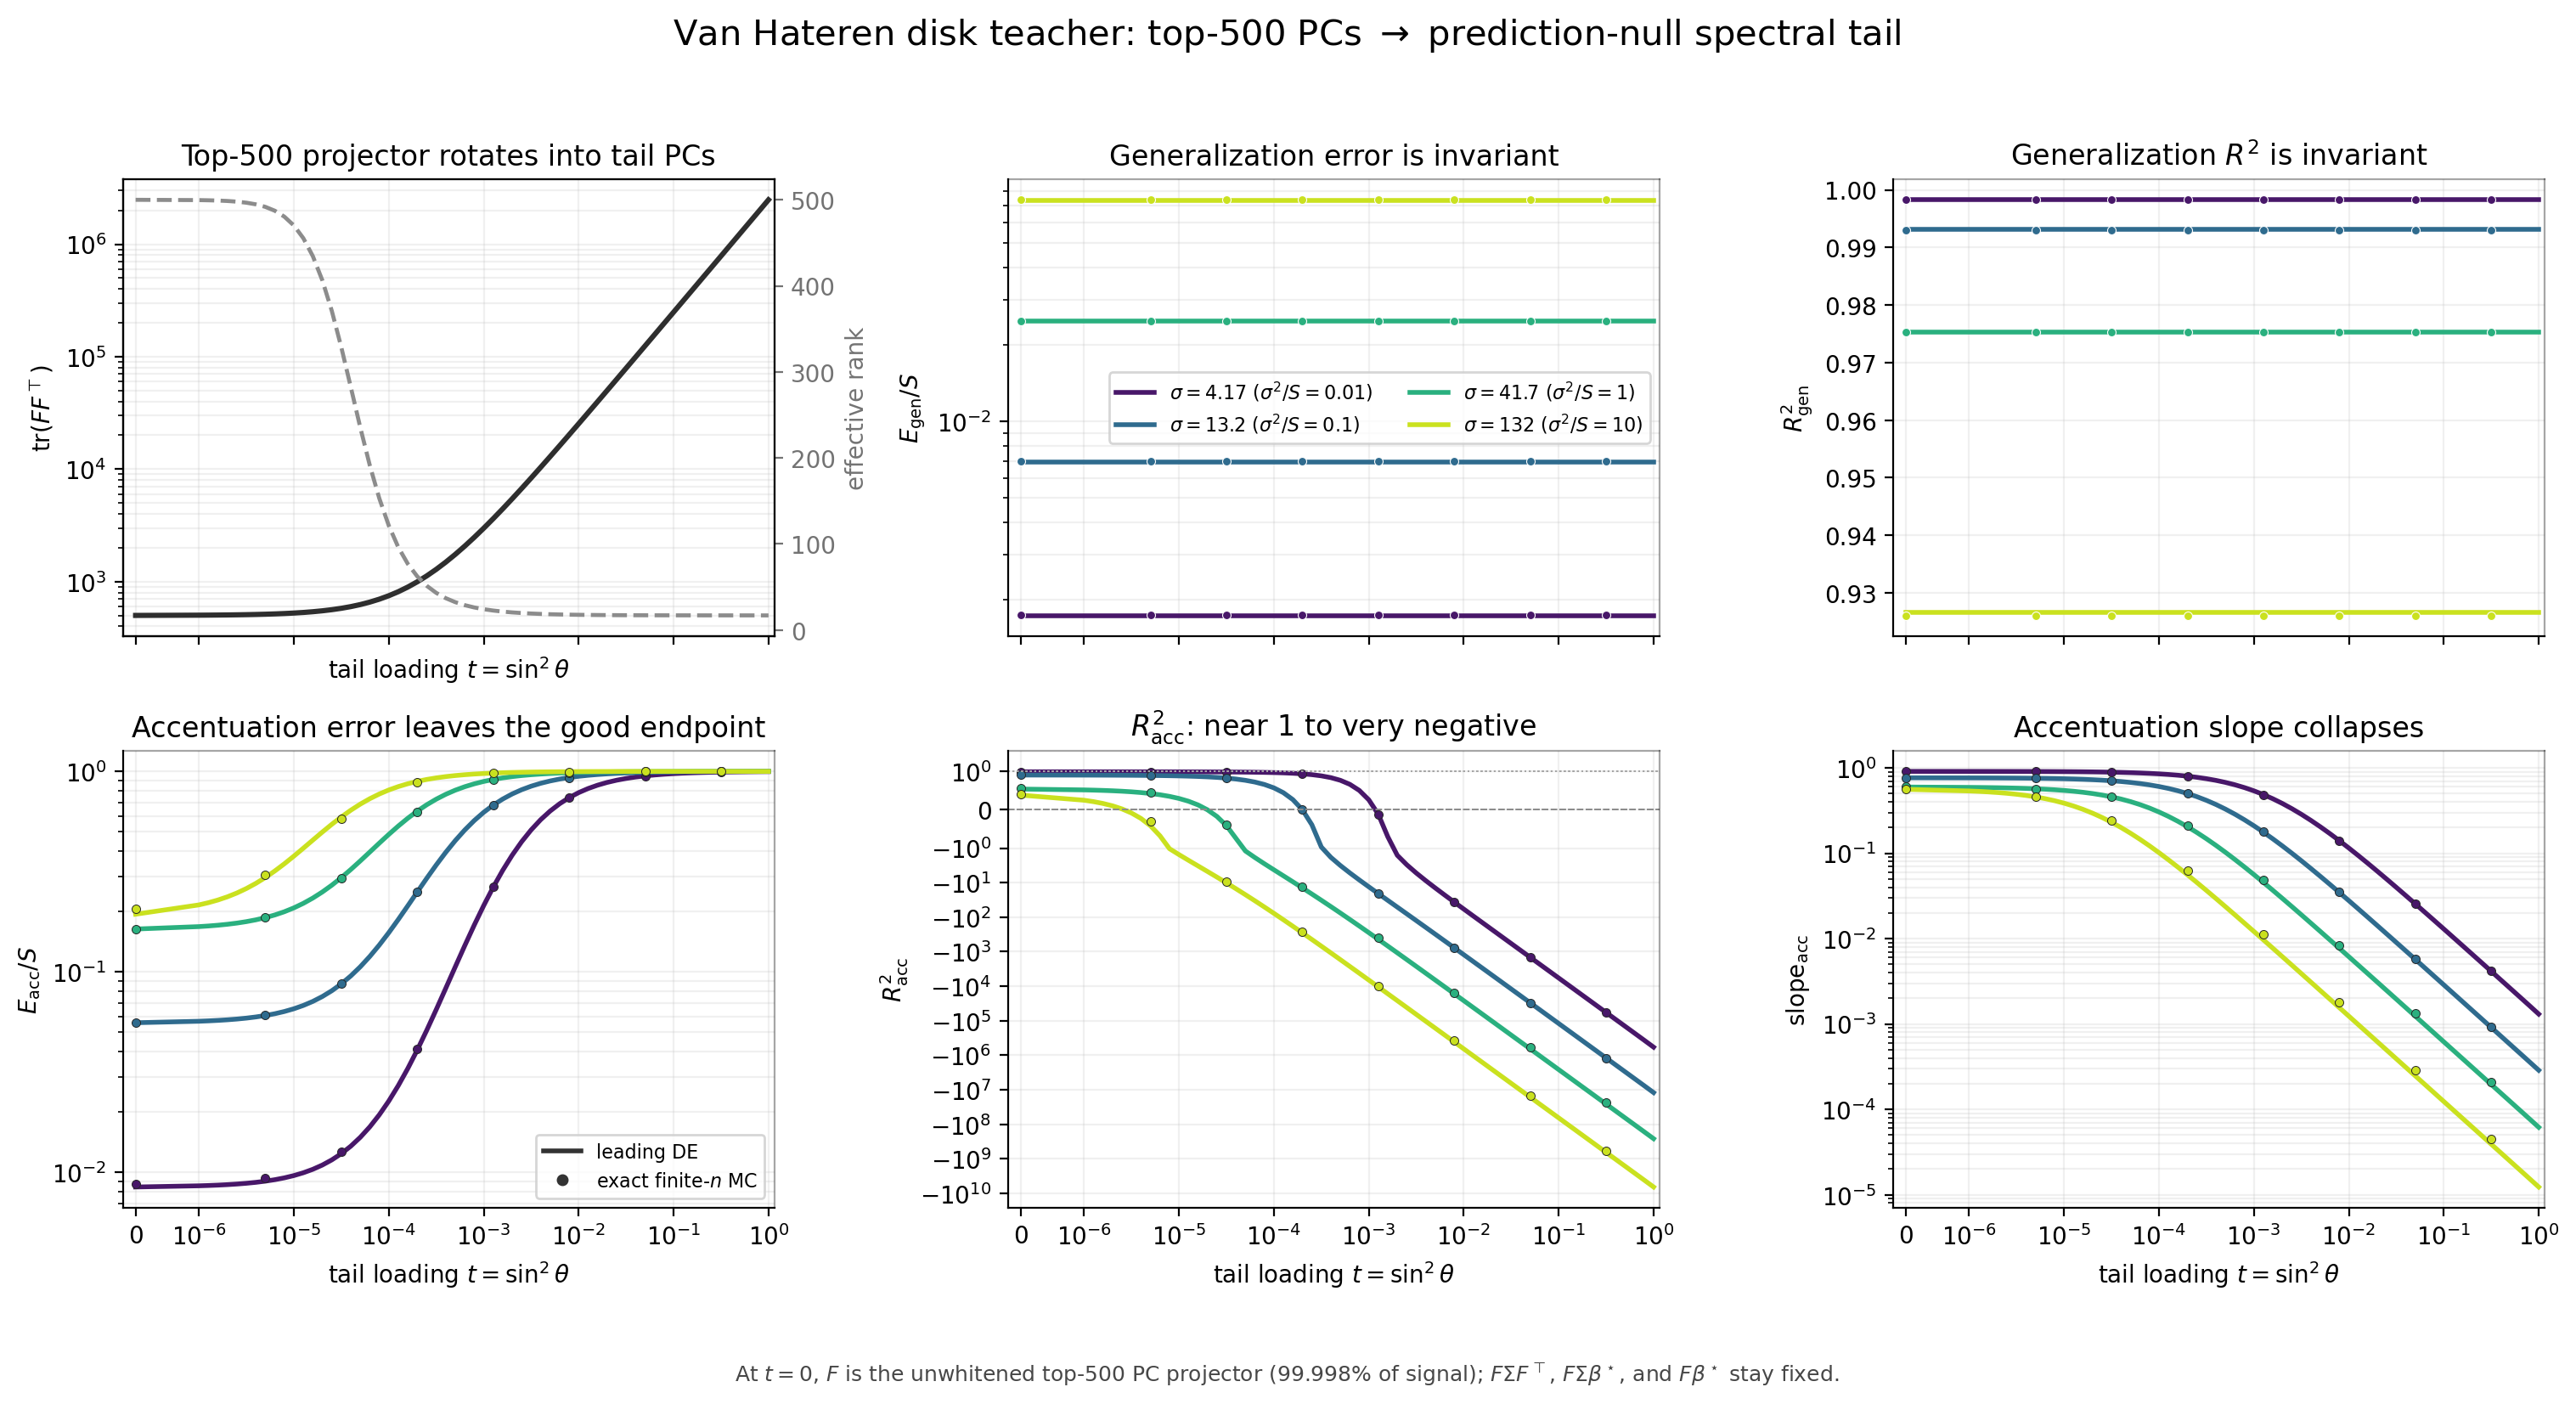
\includegraphics[clip,width=1\linewidth]{figures/VanHateren_Top500PC_prediction_null_feature_rotation}\\
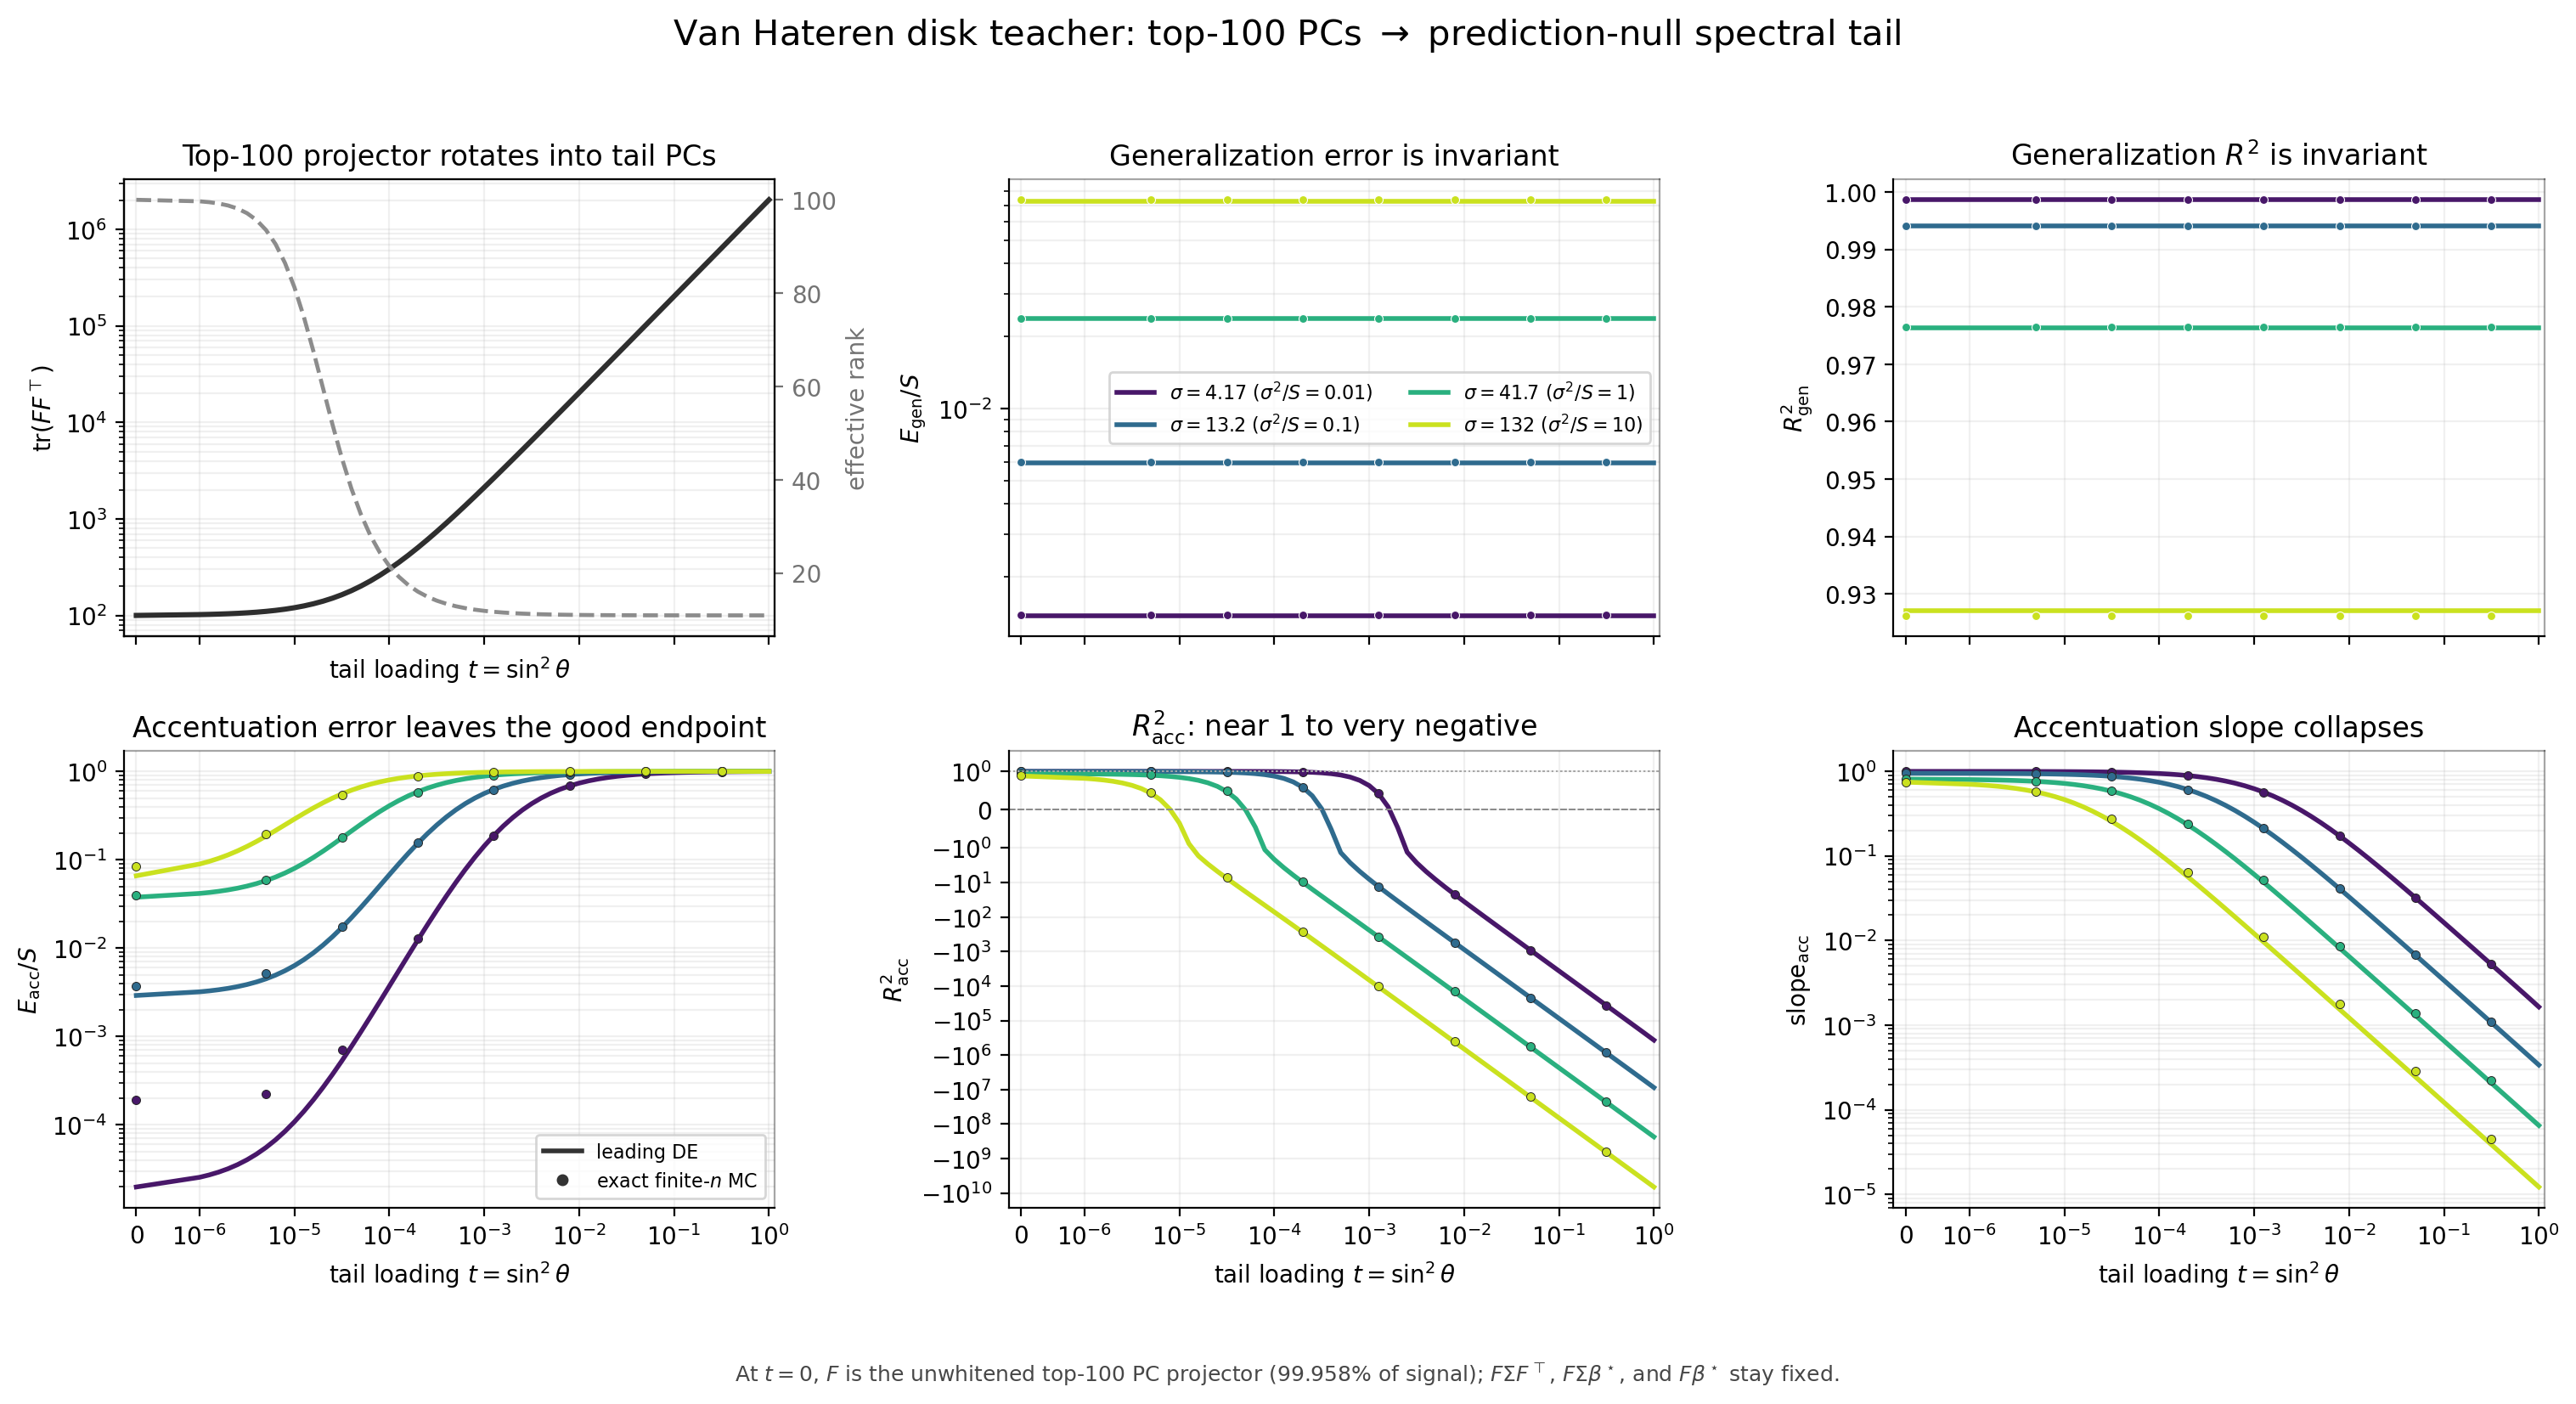
\includegraphics[width=1\linewidth]{figures/VanHateren_Top100PC_prediction_null_feature_rotation}
\par\end{centering}
\caption{Validating the }

\end{figure}


\section{Nonlinear feature and kernel regression }


\section{Appendix for deterministic equivalence and RMT}

\subsection{Deterministic equivalence relationships}

Denote $1/\varphi(-z)=\kappa(z)$

Then we have the equivalence and flip the sign of $z$
\[
\mbox{tr}\bigl[A\,(\widehat{\Sigma}+zI)^{-1}\bigr]\sim\frac{\kappa(z)}{z}\mbox{tr}\bigl[A\bigl(\Sigma+\kappa(z)I\bigr)^{-1}\bigr]
\]
\begin{align*}
\mbox{tr}\bigl[A(\widehat{\Sigma}+zI)^{-1}B(\widehat{\Sigma}+zI)^{-1}\bigr] & \sim\frac{\kappa(z)^{2}}{z^{2}\,}\mbox{tr}\bigl[A\,\bigl(\Sigma+\kappa(z)I\bigr)^{-1}\,B\,\bigl(\Sigma+\kappa(z)I\bigr)^{-1}\bigr]\\
 & \quad+\frac{\kappa(z)^{2}}{z^{2}}\frac{1}{n-\mathrm{df}_{2}\bigl(\kappa(z)\bigr)}\mbox{tr}\bigl[A\,\bigl(\Sigma+\kappa(z)I\bigr)^{-2}\Sigma\bigr]\mbox{tr}\bigl[B\,\bigl(\Sigma+\kappa(z)I\bigr)^{-2}\Sigma\bigr]
\end{align*}

Using equivalent form 
\[
\mbox{tr}\bigl[A\widehat{\Sigma}(\widehat{\Sigma}+zI)^{-1}\bigr]\sim\mbox{tr}\bigl[A\,\Sigma\,\bigl(\Sigma+\kappa(z)I\bigr)^{-1}\bigr]
\]
\begin{align*}
\mbox{tr}\bigl[A\,\widehat{\Sigma}\,(\widehat{\Sigma}+zI)^{-1}\,B\,\widehat{\Sigma}\,(\widehat{\Sigma}+zI)^{-1}\bigr] & \sim\mbox{tr}\bigl[A\,\Sigma\,\bigl(\Sigma+\kappa(z)I\bigr)^{-1}\,B\,\Sigma\,\bigl(\Sigma+\kappa(z)I\bigr)^{-1}\bigr]\\
 & \quad+\frac{\kappa^{2}(z)}{n-\mathrm{df}_{2}\bigl(\kappa(z)\bigr)}\mbox{tr}\bigl[A\,\bigl(\Sigma+\kappa(z)I\bigr)^{-2}\Sigma\bigr]\mbox{tr}\bigl[B\,\bigl(\Sigma+\kappa(z)I\bigr)^{-2}\Sigma\bigr]
\end{align*}

where $\kappa(z)$ can be solved from self consistent equation 

The self consistent variable is defined via $\varphi(z):=\mbox{tr}[(XX^{\top}-nzI)^{-1}]$,
then the self consistent equation for $\kappa(z):=\frac{1}{\varphi(-z)}$
is, where $\mu(s)$ is the spectral measure of covariance $\Sigma$
\[
\frac{1}{\varphi(z)}+z=\gamma\int_{0}^{\infty}\frac{s\ d\mu(s)}{1+s\varphi(z)}
\]
\begin{align*}
\frac{1}{\varphi(-z)}-z & =\gamma\int_{0}^{\infty}\frac{s\ d\mu(s)}{1+s\varphi(-z)}\\
\kappa(z)-z & =\gamma\int_{0}^{\infty}\frac{s\ d\mu(s)}{1+s\frac{1}{\kappa(z)}}\\
\kappa(z)-z & =\gamma\int_{0}^{\infty}\frac{\kappa(z)\ sd\mu(s)}{\kappa(z)+s}\\
\kappa(z)-z & =\gamma\kappa(z)\int_{0}^{\infty}\frac{sd\mu(s)}{\kappa(z)+s}\\
z & =\kappa(z)\Big[1-\gamma\int_{0}^{\infty}\frac{\ sd\mu(s)}{\kappa(z)+s}\Big]
\end{align*}

in matrix form 
\[
\kappa(\lambda)-\lambda=\gamma\kappa(\lambda)\!\mathrm{tr}[\Sigma(\Sigma+\kappa(\lambda))^{-1}]
\]


\paragraph{Useful quantities and identities}

\begin{align*}
\mathrm{df}_{1}(\lambda) & :=\mbox{Tr}[\Sigma(\Sigma+\lambda I)^{-1}]\\
\mathrm{df}_{2}(\lambda) & :=\mbox{Tr}[\Sigma^{2}(\Sigma+\lambda I)^{-2}]
\end{align*}

With identities
\begin{align*}
\mathrm{df}_{2}(\kappa)-\mathrm{df}_{1}(\kappa) & =\mbox{Tr}[\Sigma^{2}(\Sigma+\kappa I)^{-2}]-\mbox{Tr}[\Sigma(\Sigma+\kappa I)^{-1}]\\
 & =\mbox{Tr}[\big(\Sigma(\Sigma+\kappa I)^{-1}-I\big)\Sigma(\Sigma+\kappa I)^{-1}]\\
 & =\kappa\mbox{Tr}[\Sigma(\Sigma+\kappa I)^{-2}]
\end{align*}

We have relationship 
\[
\min(n,p)>\mathrm{df}_{2}(\kappa)>\mathrm{df}_{1}(\kappa)
\]


\paragraph{Two point equivalence}

As an immediate outcome, set $A=\Sigma$, $B=\frac{1}{n}XX^{T}$ as
white Wishart, then $A*B=\hat{\Sigma}$. Thus, 
\[
\hat{\Sigma}(\lambda+\hat{\Sigma})^{-1}M\hat{\Sigma}(\lambda^{\prime}+\hat{\Sigma})^{-1}\simeq T_{\Sigma}MT_{\Sigma}^{\prime}+\kappa\kappa'G_{\Sigma}\Sigma G_{\Sigma}^{\prime}\frac{\mbox{Tr}\left[G_{\Sigma}^{\prime}\Sigma G_{\Sigma}M\right]}{n-\mathrm{df}_{2}(\kappa,\kappa')}
\]

in trace form we can write 
\[
\mbox{Tr}\Big[A\hat{\Sigma}(\lambda+\hat{\Sigma})^{-1}B\hat{\Sigma}(\lambda^{\prime}+\hat{\Sigma})^{-1}\Big]\simeq\mbox{Tr}\big[AT_{\Sigma}BT_{\Sigma}^{\prime}\big]+\frac{\kappa\kappa'}{n-\mathrm{df}_{2}(\kappa,\kappa')}\mbox{Tr}\big[AG_{\Sigma}\Sigma G_{\Sigma}^{\prime}\big]\mbox{Tr}\big[G_{\Sigma}^{\prime}\Sigma G_{\Sigma}B\big]
\]
where $T_{A}:=A(A+\kappa)^{-1},T_{A}^{\prime}:=A(A+\kappa^{\prime})^{-1}$,
$G_{A}:=(A+\kappa)^{-1},G_{A}^{\prime}:=(A+\kappa^{\prime})^{-1}$.
and $\mathrm{df}_{2}(\kappa,\kappa'):=\mathrm{tr}[A^{2}G_{A}G_{A}^{\prime}]$,
$q=N/P$ and $A\in\mathbb{R}^{N\times N}$.

\subsection{General algebraic quantity}

In the derivation, we will heavily rely on the two family of quantities
\begin{align*}
B_{p,q}(\kappa) & =\sum_{k=1}^{d}\frac{s_{k}^{p}}{(s_{k}+\kappa)^{q}}b_{k}^{2}\\
\mathrm{df}_{p,q}(\kappa) & =\sum_{k=1}^{d}\frac{s_{k}^{p}}{(s_{k}+\kappa)^{q}}
\end{align*}

where the classic short hand are special cases of these. 
\begin{align*}
\mathrm{df}_{1}(\kappa) & \equiv\mathrm{df}_{1,1}(\kappa)\\
\mathrm{df}_{2}(\kappa) & \equiv\mathrm{df}_{2,2}(\kappa)
\end{align*}

The start of the recurssion is meaningful
\begin{align*}
\mathrm{df}_{0,0}(\kappa) & =d\\
B_{0,0}(\kappa) & =\|\beta^{\star}\|^{2}=\sum b_{k}^{2}
\end{align*}

They can be interpreted as following 
\begin{itemize}
\item $\mathrm{df}_{p,q}(\kappa)$ is a weighted \textbf{count} of spectral
modes, where the weighting function is $\frac{s_{k}^{p}}{(s_{k}+\kappa)^{q}}$.
In classic cases $p=q$ and these weighting functions range from $(0,1)$
so it's exactly counting the modes from 0,1. 
\end{itemize}

\subsubsection{Inequalities}

Since $\kappa>0$, 
\[
\frac{s_{k}}{(s_{k}+\kappa)}<1
\]

thus in general 
\begin{align*}
B_{p,q}(\kappa) & \geq B_{p+1,q+1}(\kappa)\\
\mathrm{df}_{p,q}(\kappa) & \geq\mathrm{df}_{p+1,q+1}(\kappa)
\end{align*}

The classic inequality of 
\[
d\geq\mathrm{df}_{1}(\kappa)\geq\mathrm{df}_{2}(\kappa)
\]

can be seen as a special case of 
\[
\mathrm{df}_{0,0}(\kappa)\geq\mathrm{df}_{1,1}(\kappa)\geq\mathrm{df}_{2,2}(\kappa)
\]

Here we have the more general case 
\[
\mathrm{df}_{0,1}(\kappa)\geq\mathrm{df}_{1,2}(\kappa)\geq\mathrm{df}_{2,3}(\kappa)
\]


\subsubsection{Recursion and Differential Identities}

They admits following recursion identities, 
\[
\mathrm{df}_{p,q}(\kappa)=\mathrm{df}_{p+1,q+1}(\kappa)+\kappa\mathrm{df}_{p,q+1}(\kappa)
\]

Equivalently 
\begin{align*}
\mathrm{df}_{p+1,q+1}(\kappa)-\mathrm{df}_{p,q}(\kappa) & =-\kappa\mathrm{df}_{p,q+1}(\kappa)\\
B_{p+1,q+1}(\kappa)-B_{p,q}(\kappa) & =-\kappa B_{p,q+1}(\kappa)
\end{align*}
\begin{align*}
\partial_{\kappa}\mathrm{df}_{p,q}(\kappa) & =-q\sum_{k=1}^{d}\frac{s_{k}^{p}}{(s_{k}+\kappa)^{q+1}}\\
 & =-q\mathrm{df}_{p,q+1}(\kappa)
\end{align*}
\begin{align*}
\partial_{\kappa}\big(\kappa^{r}\mathrm{df}_{p,q}(\kappa)\big) & =r\kappa^{r-1}\mathrm{df}_{p,q}(\kappa)-q\kappa^{r}\mathrm{df}_{p,q+1}(\kappa)\\
 & =r\kappa^{r-1}\sum_{k=1}^{d}\frac{s_{k}^{p}(s_{k}+\kappa)}{(s_{k}+\kappa)^{q+1}}-q\kappa^{r}\mathrm{df}_{p,q+1}(\kappa)\\
 & =r\kappa^{r-1}\sum_{k=1}^{d}\frac{s_{k}^{p+1}}{(s_{k}+\kappa)^{q+1}}+r\kappa^{r}\sum_{k=1}^{d}\frac{s_{k}^{p}}{(s_{k}+\kappa)^{q+1}}-q\kappa^{r}\mathrm{df}_{p,q+1}(\kappa)\\
 & =r\kappa^{r-1}\mathrm{df}_{p+1,q+1}(\kappa)+(r-q)\kappa^{r}\mathrm{df}_{p,q+1}(\kappa)
\end{align*}


% \end{document}
